\documentclass[a4paper, 11pt, titlepage]{article}
\usepackage[slovene]{babel}
\usepackage[utf8]{inputenc}
\usepackage[slovene]{babelbib}
\usepackage{lmodern}
\usepackage[T1]{fontenc}
\usepackage{microtype}
\usepackage{chngcntr}
\usepackage{environ}
\usepackage{needspace}
\usepackage[small]{caption}
%%%%%%%%%%%%%%%%%%%%%%%%%%%%%%%%%%%%%%%%%%%%%%%%%%%%%%%%
\usepackage{amsmath,amssymb,amstext,wasysym,mathtools}
\usepackage{algorithmicx,algpseudocode}
%%%%%%%%%%%%%%%%%%%%%%%%%%%%%%%%%%%%%%%%%%%%%%%%%%%%%%%%
\usepackage{tabularx}
\usepackage{enumerate}
\usepackage{hyperref}
\usepackage{eurosym}
\usepackage{tikz}
\usepackage{pgflibraryshapes}
\usetikzlibrary{calc}
\usetikzlibrary{matrix}
\usetikzlibrary{decorations.pathmorphing}
%%%%%%%%%%%%%%%%%%%%%%%%%%%%%%%%%%%%%%%%%%%%%%%%%%%%%%%%
\newcommand{\A}{\ensuremath{\mathcal{A}}}
\newcommand{\N}{\ensuremath{\mathbb{N}}}
\newcommand{\R}{\ensuremath{\mathbb{R}}}
\newcommand{\Z}{\ensuremath{\mathbb{Z}}}
\newcommand{\p}{\ensuremath{\mathcal{P}}}
\newcommand{\set}[2]{\ensuremath{\left\{ #1 \; \middle| \; #2 \right\}}}
\newcommand{\mm}{\ensuremath{\phantom{|}-\phantom{|}}}
\newcommand{\pp}{\ensuremath{\phantom{|}+\phantom{|}}}
%%%%%%%%%%%%%%%%%%%%%%%%%%%%%%%%%%%%%%%%%%%%%%%%%%%%%%%%
\newcommand{\razdelek}[2][7]{\needspace{#1\baselineskip}\subsection{#2}}
\newcommand{\opis}[2][2]{\shortintertext{\small\needspace{#1\baselineskip}#2:}}
%%%%%%%%%%%%%%%%%%%%%%%%%%%%%%%%%%%%%%%%%%%%%%%%%%%%%%%%
\DeclareUnicodeCharacter{20AC}{\euro}
\DeclareRobustCommand{\officialeuro}{%
  \ifmmode\expandafter\text\fi
  {\fontencoding{U}\fontfamily{eurosym}\selectfont e}}
\newcommand{\ME}{\ensuremath{\operatorname{M€}}}
%%%%%%%%%%%%%%%%%%%%%%%%%%%%%%%%%%%%%%%%%%%%%%%%%%%%%%%%
%% https://tex.stackexchange.com/questions/51733/global-renewcommand-equivalent-of-global-def/51751#51751
\makeatletter
\def\gnewcommand{\g@star@or@long\new@command}
\def\grenewcommand{\g@star@or@long\renew@command}
\def\g@star@or@long#1{%
  \@ifstar{\let\l@ngrel@x\global#1}{\def\l@ngrel@x{\long\global}#1}}
\makeatother

\newcounter{naloga}
\counterwithin*{naloga}{subsection}
\renewcommand{\thenaloga}{\arabic{subsection}.\arabic{naloga}}
\newenvironment{naloga}[3][]{\refstepcounter{naloga}\avtor{#2}\naslov{#1}\vir{#3}\needspace{3\baselineskip}\noindent {\bf Naloga}}{\bigskip}
\newenvironment{slika}[1][t]{\begin{figure}[#1]\centering}{\label{fig:\thislabel}\end{figure}}
\newenvironment{tabela}[1][t]{\begin{table}[#1]\centering}{\label{tab:\thislabel}\end{table}}
\newcommand{\pgfslika}{\leavevmode\beginpgfgraphicnamed{fig-\thislabel}\input{slike/\thislabel.tikz}\endpgfgraphicnamed}
\newcommand{\oznaka}[1]{\if\relax\detokenize{#1}\relax\grenewcommand{\thislabel}{\thenaloga}\else\grenewcommand{\thislabel}{#1}\fi}
\newcommand{\taoznaka}[1]{\if\relax\detokenize{#1}\relax\thislabel\else#1\fi}

\newcommand{\taavtor}{}
\newcommand{\tanaslov}{}
\newcommand{\tavir}{}
\newcommand{\thislabel}{?}
\newcommand{\nal}[1]{\ref{nal:\taoznaka{#1}}}
\newcommand{\fig}[1]{\ref{fig:\taoznaka{#1}}}
\newcommand{\tab}[1]{\ref{tab:\taoznaka{#1}}}
\newcommand{\res}[1]{\ref{res:\taoznaka{#1}}}
\newcommand{\podnaslov}[2][]{\caption{#2 za nalogo~\if\relax\detokenize{#1}\relax\del{}\else#1\fi.}}

\begin{document}
\title{Zbirka nalog iz Operacijskih raziskav}
\author{Janoš Vidali}
\maketitle

\section{Naloge}
{
\newcommand{\del}{\nal}
\newcommand{\avtor}[1]{\renewcommand{\taavtor}{\hfill {\small Avtor: #1}\par}}
\newcommand{\naslov}[1]{\renewcommand{\tanaslov}{\if\relax\detokenize{#1}\relax\else\noindent {\small\bf (#1)}\fi}}
\newcommand{\vir}[1]{\renewcommand{\tavir}{\hfill {\small Vir: #1}\par}}
\newenvironment{vprasanje}[1][]{\oznaka{#1}\label{nal:\thislabel}{\bf \res{}.}\taavtor\tanaslov\tavir\smallskip\noindent\ignorespaces}{}
\NewEnviron{odgovor}{}
\razdelek{Zahtevnost algoritmov}

\begin{naloga}{Janoš Vidali}{Vaje OR 21.2.2018}
\begin{vprasanje}
Naj bo $A[1 \dots n][1 \dots n]$ matrika (tj., seznam seznamov)
dimenzij $n \times n$.
Dan je spodnji program:
\begin{small}
\begin{algorithmic}
\For{$i = 1, \dots, n$}
    \For{$j = i+1, \dots, n$}
        \State $A[i][j] \gets A[j][i]$
    \EndFor
\EndFor
\end{algorithmic}
\end{small}

\begin{enumerate}[(a)]
\item Kaj počne zgornji program?
\item Oceni število korakov, ki jih opravi zgornji program,
v odvisnosti od parametra $n$.
\end{enumerate}
\end{vprasanje}

\begin{odgovor}
\begin{enumerate}[(a)]
\item Program prepiše vnose v matriki $A$ nad diagonalo
na ustrezno mesto pod diagonalo tako,
da je po izvedbi programa matrika $A$ simetrična.
\item Kot korak bomo upoštevali posamezno izvedbo notranje zanke {\bf for},
kjer kopiramo vrednost v matriki na drugo mesto
-- ob predpostavki, da je velikost vnosov omejena
(npr.~32-bitna cela števila),
bo trajanje take operacije omejeno s konstanto.
Preštejmo število takih korakov:
$$
\sum_{i=1}^n \sum_{j=i+1}^n 1 = \sum_{i=1}^n (n-i) = \sum_{i=0}^{n-1} i =
{n(n-1) \over 2}
$$

Lahko bi seveda upoštevali še korake,
ki so potrebni za vzdrževanje števcev zank
(inicializacija števca, povečevanje števca, preverjanje konca zanke),
a bi spet dobili kvadratni polinom v $n$.
Tako lahko rečemo, da je število korakov omejeno z $O(n^2)$.
\end{enumerate}
\end{odgovor}
\end{naloga}


\begin{naloga}{Janoš Vidali}{Vaje OR 21.2.2018}
\begin{vprasanje}
Naj bo $\ell[1 \dots n]$ seznam,
ki ima na začetku vse vrednosti nastavljene na $0$.
Dan je spodnji program:

\begin{small}
\begin{algorithmic}
\State $i \gets 1$
\While{$i \le n$}
    \State $\ell[i] \gets 1 - \ell[i]$
    \If{$\ell[i] = 1$}
        \State $i \gets 1$
    \Else
        \State $i \gets i+1$
    \EndIf
\EndWhile
\end{algorithmic}
\end{small}

\begin{enumerate}[(a)]
\item Kaj se dogaja, ko teče zgornji program?
\item Oceni število korakov, ki jih opravi zgornji program,
v odvisnosti od parametra $n$.
\end{enumerate}
\end{vprasanje}

\begin{odgovor}
\begin{enumerate}[(a)]
\item V vsakem obhodu zanke {\bf while}
se vrednost $\ell[i]$ spremeni iz $0$ v $1$ ali obratno.
Če se vrednost spremeni na $1$, se $i$ nastavi na $1$,
sicer se pa poveča za $1$.

Izpišimo si vrednosti v seznamu $\ell$ in spremenljivke $i$
ob koncu vsakega obhoda zanke {\bf while} tekom izvajanja algoritma,
recimo za $n = 4$:
$$
\begin{array}{c|c|ccc|c|c}
\text{obhod} & \ell[4 \dots 1] & i &\qquad&
\text{obhod} & \ell[4 \dots 1] & i \\ \cline{1-3} \cline{5-7}
 1 & 0001 & 1 && 16 & 1001 & 1 \\
 2 & 0000 & 2 && 17 & 1000 & 2 \\
 3 & 0010 & 1 && 18 & 1010 & 1 \\
 4 & 0011 & 1 && 19 & 1011 & 1 \\
 5 & 0010 & 2 && 20 & 1010 & 2 \\
 6 & 0000 & 3 && 21 & 1000 & 3 \\
 7 & 0100 & 1 && 22 & 1100 & 1 \\
 8 & 0101 & 1 && 23 & 1101 & 1 \\
 9 & 0100 & 2 && 24 & 1100 & 2 \\
10 & 0110 & 1 && 25 & 1110 & 1 \\
11 & 0111 & 1 && 26 & 1111 & 1 \\
12 & 0110 & 2 && 27 & 1110 & 2 \\
13 & 0100 & 3 && 28 & 1100 & 3 \\
14 & 0000 & 4 && 29 & 1000 & 4 \\
15 & 1000 & 1 && 30 & 0000 & 5 \\
\end{array}
$$
Če pogledamo samo tiste obhode, na koncu katerih velja $i = 1$, opazimo,
da vrednosti v seznamu $\ell$ predstavljajo
dvojiške zapise števil od $1$ do $2^n - 1$
v ostalih pa se najmanj pomembna $1$ zamenja z $0$.
Algoritem torej simulira dvojiški števec z $n$ mesti.

\item Algoritem obišče vseh $2^n - 1$ števil,
poleg tega pa mora vsakič poskrbeti za zamenjavo vseh enic
za najmanj pomembno ničlo.
Ob upoštevanju, da obstaja $2^{n-i}$ števil
z najmanj pomembno ničlo na $i$-tem mestu,
za vrednost $2^n - 1$ pa je potrebno nadomestiti vseh $n$ mest,
je skupno število korakov enako
\begin{multline*}
n + \sum_{i=1}^n (i \cdot 2^{n-i}) =
\sum_{j=1}^n \left(1 + \sum_{i=j}^n 2^{n-i}\right) = \\
= \sum_{j=1}^n \left(1 + \sum_{i=0}^{n-j} 2^i\right) =
\sum_{j=1}^n 2^{n-j+1} = 2^{n+1} - 2 .
\end{multline*}
Časovna zahtevnost algoritma je torej $O(2^n)$.
\end{enumerate}
\end{odgovor}
\end{naloga}


\begin{naloga}{Janoš Vidali}{Vaje OR 21.2.2018}
\begin{vprasanje}
Algoritem {\sc BubbleSort} uredi vhodni seznam $\ell[1 \dots n]$ tako,
da zamenjuje sosednje elemente v nepravem vrstnem redu:
\begin{small}
\begin{algorithmic}
\Function{BubbleSort}{$\ell[1 \dots n]$}
    \State $z \gets n$
    \While{$z > 1$}
        \State $y \gets 1$
        \For{$i = 2, \dots, z$}
            \If{$\ell[i-1] > \ell[i]$}
                \State $\ell[i-1], \ell[i] \gets \ell[i], \ell[i-1]$
                \State $y \gets i$
            \EndIf
        \EndFor
        \State $z \gets y-1$
    \EndWhile
\EndFunction
\end{algorithmic}
\end{small}

\begin{enumerate}[(a)]
\item Izvedi algoritem na seznamu $[7, 11, 16, 7, 5]$.
\item Določi časovno zahtevnost algoritma.
\end{enumerate}
\end{vprasanje}

\begin{odgovor}
\begin{enumerate}[(a)]
\item Izpišimo vrednosti spremenljivk ob koncu vsakega obhoda zanke {\bf for}
oziroma {\bf while}, ko se prejšnja konča.

$$
\begin{array}{c|c|c|c|c}
\text{obhod {\bf while}} & i & y & z & \ell[1 \dots 5] \\ \hline
1 & 2 & 1 & 5 & [7, 11, 16, 7, 5] \\
1 & 3 & 1 & 5 & [7, 11, 16, 7, 5] \\
1 & 4 & 4 & 5 & [7, 11, 7, 16, 5] \\
1 & 5 & 5 & 5 & [7, 11, 7, 5, 16] \\
1 &   & 5 & 4 & [7, 11, 7, 5, 16] \\
2 & 2 & 1 & 4 & [7, 11, 7, 5, 16] \\
2 & 3 & 3 & 4 & [7, 7, 11, 5, 16] \\
2 & 4 & 4 & 4 & [7, 7, 5, 11, 16] \\
2 &   & 4 & 3 & [7, 7, 5, 11, 16] \\
3 & 2 & 1 & 3 & [7, 7, 5, 11, 16] \\
3 & 3 & 3 & 3 & [7, 5, 7, 11, 16] \\
3 &   & 3 & 2 & [7, 5, 7, 11, 16] \\
4 & 2 & 2 & 2 & [5, 7, 7, 11, 16] \\
4 &   & 2 & 1 & [5, 7, 7, 11, 16] \\
\end{array}
$$

\item Naj bodo $z_1, z_2, \dots, z_k$ vrednosti,
ki jih zavzame spremenljivka $z$ ob vsakem vstopu v zanko {\bf while}.
Očitno velja $z_i - 1 \ge z_{i+1}$ za vsak $i$,
tako da velja $k \le n-1$.
Največje število korakov je torej
$$
\sum_{z=2}^n (z-1) = {n(n-1) \over 2} .
$$
Tako število korakov dosežemo,
če je seznam $\ell$ na začetku urejen padajoče
-- tako vsakič pride do zamenjave v zadnjem koraku zanke {\bf for},
zato se $z$ vsakič zmanjša za $1$.
Časovna zahtevnost algoritma je torej $O(n^2)$.
\end{enumerate}
\end{odgovor}
\end{naloga}


\begin{naloga}{Janoš Vidali}{Vaje OR 12.10.2016}
\begin{vprasanje}[mergesort]
Algoritem {\sc MergeSort} uredi vhodni seznam tako,
da ga najprej razdeli na dva dela,
nato vsakega rekurzivno uredi,
nazadnje pa zlije dobljena urejena seznama.
\begin{enumerate}[(a)]
\item S psevdokodo zapiši algoritem {\sc MergeSort}.
\item Izvedi algoritem na seznamu $[7, 11, 16, 7, 5, 0, 14, 1, 19, 13]$.
\item Določi časovno zahtevnost algoritma.
\end{enumerate}
\end{vprasanje}

\begin{odgovor}
\begin{enumerate}[(a)]
\item
\begin{small}
\begin{algorithmic}
\Function{MergeSort}{$\ell[1 \dots n]$}
    \If{$n \le 1$}
        \State \Return $\ell$
    \EndIf
    \State $m \gets \lceil {n \over 2} \rceil$
    \State $\ell_1 \gets \text{\sc MergeSort}(\ell[1 \dots m])$
    \State $\ell_2 \gets \text{\sc MergeSort}(\ell[m+1 \dots n])$
    \State $i, j \gets 1, 1$
    \State $\ell' \gets []$
    \While{$i \le m \land j \le n-m$}
        \If{$\ell_1[i] \le \ell_2[j]$}
            \State dodaj $\ell_1[i]$ na konec $\ell'$
            \State $i \gets i+1$
        \Else
            \State dodaj $\ell_2[j]$ na konec $\ell'$
            \State $j \gets j+1$
        \EndIf
    \EndWhile
    \State pripni $\ell_1[i \dots m]$ na konec $\ell'$
    \State pripni $\ell_2[j \dots n-m]$ na konec $\ell'$
    \State \Return $\ell'$
\EndFunction
\end{algorithmic}
\end{small}

\item Izvajanje algoritma je prikazano na sliki~\fig{}.
Nad črtkano črto je prikazano rekurzivno razbijanje seznamov,
pod njo pa zlivanje dobljenih urejenih podseznamov.

\item Funkcija obsega dva rekurzivna klica na seznamih polovične dolžine
ter združevanje obeh dobljenih seznamov v enega.
Naj bo $T(n)$ čas izvajanja algoritma pri vhodnem seznamu dolžine $n$.
Ker združevanje poteka v linearnem času, velja rekurzivna zveza
$$
T(n) = O(n) + 2T\left({n \over 2}\right) .
$$
Po krovnem izreku lahko izpeljemo,
da je časovna zahtevnost algoritma $O(n \log n)$.
\end{enumerate}

\begin{slika}
\pgfslika
\podnaslov[\res{}(b)]{Diagram izvajanja algoritma}
\end{slika}
\end{odgovor}
\end{naloga}


\begin{naloga}{Janoš Vidali}{Vaje OR 21.2.2018}
\begin{vprasanje}
Število $n$ želimo razcepiti
na dva netrivialna celoštevilska faktorja,
kar storimo s sledečim algoritmom:
\begin{small}
\begin{algorithmic}
\Function{Razcep}{$n$}
    \For{$i = 2, \dots, \lfloor \sqrt{n} \rfloor$}
        \If{$n/i$ je celo število}
            \State \Return $(i, n/i)$
        \EndIf
    \EndFor
    \State \Return $n$ je praštevilo
\EndFunction
\end{algorithmic}
\end{small}
Določi časovno zahtevnost algoritma.
Ali je ta algoritem polinomski?
\end{vprasanje}

\begin{odgovor}
Algoritem teče v času $O(\sqrt{n})$.
Ker je vhod algoritma število $n$,
ki je zapisano kot zaporedje $\ell = O(\log n)$ bitov,
vidimo, da algoritem teče v času $O(2^{\ell/2})$
in torej ni polinomski v dolžini vhoda.
\end{odgovor}
\end{naloga}


\begin{naloga}{Janoš Vidali}{Vaje OR 21.2.2018}
\begin{vprasanje}
Zapiši rekurziven algoritem,
ki na vhod dobi celo število $n$ in teče v času $O(\sqrt{n})$.
Uporaba korenjenja ni dovoljena.
\end{vprasanje}

\begin{odgovor}
Po krovnem izreku ima časovno zahtevnost $O(\sqrt{n})$ algoritem,
katerega čas izvajanja $T(n)$ je opisan z rekurzivno zvezo
$$
T(n) = O(1) + 2T\left({n \over 4}\right) .
$$
Zapišimo tak algoritem:
\begin{small}
\begin{algorithmic}
\Function{Korenski}{$\ell[1 \dots n]$}
    \If{$n \ge 4$}
        \State $m \gets \lfloor {n \over 4} \rfloor$
        \State $\text{\sc Korenski}(\ell[1 \dots m])$
        \State $\text{\sc Korenski}(\ell[n-m+1 \dots n])$
    \EndIf
\EndFunction
\end{algorithmic}
\end{small}
\end{odgovor}
\end{naloga}


\begin{naloga}{?}{Kolokvij OR 17.4.2013}
\begin{vprasanje}
Dani so končna neprazna množica $S \subset \N$ moči $n$,
število $k \in \{1, 2, \dots, n\}$ ter algoritem {\sc Alg}:
\begin{small}
\begin{algorithmic}
\Function{Alg}{$S, k$}
    \State $x \gets$ naključen element $S$
    \State $S^+ \gets \set{y \in S}{y > x}$
    \State $S^- \gets \set{y \in S}{y < x}$
    \If{$|S^-| < k-1$}
        \State \Return {\sc Alg}$(S^+, k - |S^-| - 1)$
    \ElsIf{$|S^-| = k-1$}
        \State \Return $x$
    \Else
        \State \Return {\sc Alg}$(S^-, k)$
    \EndIf
\EndFunction
\end{algorithmic}
\end{small}
Ugotovi, kaj je izhod algoritma pri danih vhodnih podatkih $S$ in $k$.
Oceni časovno zahtevnost algoritma v najslabšem in v povprečnem primeru.
\end{vprasanje}

\begin{odgovor}
Algoritem poišče $k$-ti najmanjši element v množici $S$.
Množico razdeli na dva dela glede na naključno izbrani element $x$.
Če ima množica $S^-$ elementov, manjših od $x$, natanko $k-1$ elementov,
potem je $x$ iskani element.
Če ima $S^-$ manj kot $k-1$ elementov,
algoritem rekurzivno poišče $(|S^-| - k - 1)$-ti element
v množici $S^+$ elementov, večjih od $x$,
sicer pa rekurzivno poišče $k$-ti element v množici $|S^-|$.

V najslabšem primeru je velikost množice,
ki jo algoritem rekurzivno preišče, enaka $n - 1$.
Ker algoritem porabi $O(n)$ korakov za razporejanje elementov po množicah,
v najslabšem primeru za čas izvajanja $T(n)$ velja
$$
T(n) = O(n) + T(n-1) = O\left(\sum_{i=0}^n (n-i)\right) = O(n^2).
$$

Poglejmo si sedaj povprečni čas izvajanja $\hat{T}(n)$.
Denimo, da je izbrani element $x$ $j$-ti po vrsti.
Če velja $j = k$, potem algoritem konča.
Če velja $j < k$, potem algoritem rekurzivno pregleda
množico $S^+$ z $n-j$ elementi,
če pa velja $j > k$, pa pregleda množico $S^-$ z $j-1$ elementi.
Zapišimo rekurzivno zvezo za $\hat{T}(n)$:
$$
\hat{T}(n) = O(n) +
{1 \over n} \left(\sum_{j=1}^{k-1} \hat{T}(n-j) +
\sum_{j=k+1}^n \hat{T}(j-1) \right)
$$
Denimo, da je čas izvajanja nerekurzivnega dela funkcije
omejen s $c \cdot n$ koraki za neko konstanto $c > 0$.
Z indukcijo bomo pokazali,
da velja $\hat{T}(n) \le C \cdot n$ za neko konstanto $C > 0$.

Po zgornji predpostavki velja $\hat{T}(1) \le cn$.
Denimo, da za vse $m < n$ velja $\hat{T}(m) \le Cm$.
Potem velja
\begin{align*}
\hat{T}(n) &\le cn +
{1 \over n} \left(\sum_{j=1}^{k-1} C(n-j) +
\sum_{j=k+1}^n C(j-1) \right) \\
&= cn + {C \over 2n} ((2n-k)(k-1) + (n+k-1)(n-k)) \\
&= cn + {C \over 2n} (n^2 + 2nk - 3n - 2k^2 + 2k) \\
&= \left(c + {C \over 2}\right) n + {C(2k - 3) \over 2} - {Ck(k-1) \over n}
\end{align*}
Označimo sedaj $\alpha = k/n$ -- velja torej $0 < \alpha \le 1$.
\begin{align*}
\hat{T}(n) &\le
\left(c + C \left({1 \over 2} + \alpha - \alpha^2\right) \right) n
+ C \left(\alpha - {3 \over 2}\right) \\
&\le \left(c + C \left({1 \over 2} + \alpha (1 - \alpha)\right) \right) n \\
&\le \left(c + {3C \over 4} \right) n
\end{align*}
Če vzamemo $C \ge 4c$,
potem po indukciji velja $\hat{T}(n) \le Cn$ za vse $n$.
Algoritem torej v povprečnem primeru opravi $O(n)$ korakov.
\end{odgovor}
\end{naloga}

\begin{naloga}{?}{Kolokvij OR 25.11.2010}
\begin{vprasanje}
\begin{enumerate}[(a)]
\item Dokaži, da za poljubni konstanti $a, b \in \R$, kjer je $b > 0$,
velja ${(n + a)}^b = O(n^b)$.

\item Naj bo $f$ naraščajoča funkcija.
Ali velja $g(n) = O(f(g(n)))$?

\item Dokaži,
da če $T$ zadošča pogoju $T(n) = 2T(\lceil n/2 \rceil) - 13$ za $n \ge 2$,
potem je $T(n) = O(n)$.
\end{enumerate}
\end{vprasanje}
\begin{odgovor}
\end{odgovor}
\end{naloga}

\subsection{Celoštevilsko linearno programiranje}

\begin{naloga}{}{?}{Vaje OR 16.3.2016}
\begin{vprasanje}
\label{nal:proj}
Občina Ljubljana želi projekte iz množice
$\p = \{p_1, p_2, \dots, p_n\}$,
pri čemer ima na voljo $M$ evrov kapitala.
V želji po razvoju regije želijo,
da se v sklopu sponzoriranih projektov ustvari vsaj $N$ delovnih mest.
Projekt $p_i$ ($1 \le i \le n)$ potrebuje $d_i$ evrov finančne pomoči
in zaposli $a_i$ ljudi.
Na občini so ocenili,
da ima projekt $p_i$ ob uspešnem dokončanju donos $c_i$ evrov.
Katere projekte naj sponzorira, da bo donos čim večji?
Na smiseln način modeliraj opisani problem z linearnim programom.
\end{vprasanje}
\begin{odgovor}
\end{odgovor}
\end{naloga}


\begin{naloga}{}{?}{Vaje OR 16.3.2016}
\begin{vprasanje}
Obravnavajmo posplošen scenarij iz naloge~\ref{nal:proj}.
\begin{enumerate}[(a)]
\item Denimo, da so projekti lahko med seboj odvisni.
Imejmo množico $V \subseteq \p^2$, ki določa,
da za vsak par projektov $(p_i, p_j) \in V$ velja,
da lahko projekt $p_i$ sponzoriramo le,
če sponzoriramo tudi projekt $p_j$.

\item Nekateri izmed projektov so lahko v konfliktu.
Naj bo $S \subseteq 2^\p$ družina množic, ki določa,
da so za vsako množico $H \in S$ projekti iz $H$ med seboj v konfliktu
(tj., hkrati lahko sponzoriramo le enega izmed njih.)
\end{enumerate}
Opiši, kako bi modelirali opisane omejitve.
\end{vprasanje}
\begin{odgovor}
\end{odgovor}
\end{naloga}


\begin{naloga}{problem prevoza in skladiščenja dobrin}{?}{Vaje OR 16.3.2016}
\begin{vprasanje}
V Evropski uniji je na voljo $n$ skladišč,
pri čemer znašajo stroški najema $i$-tega skladišča $f_i$
(ne glede na zasedenost),
vsako skladišče pa lahko hrani enoto dobrine.
Imamo $m$ strank, ki jim dostavljamo dobrine,
pri čemer $c_{ij}$ ($1 \le i \le n$, $1 \le j \le m$)
predstavlja strošek dostave dobrine stranki $j$ iz skladišča $i$.
Predpostavimo tudi, da ima vsaka stranka določeno potrebo $d_j$,
ki ponazarja število enot dobrine, ki jo potrebuje.
V katerih skladiščih naj hranimo dobrine,
da bodo skupni stroški najema in dostave čim manjši?
Na smiseln način modeliraj opisani problem z linearnim programom.
\end{vprasanje}
\begin{odgovor}
\end{odgovor}
\end{naloga}


\begin{naloga}{problem kombinatorične dražbe}{Janoš Vidali}{Vaje OR 5.3.2018}
\begin{vprasanje}
Dražitelj ponuja predmete iz množice $A$
in prejme ponudbe $\{(B_i, c_i)\}_{i=1}^k$,
pri čemer je $c_i$ cena,
ki jo udeleženec dražbe ponudi za predmete v množici $B_i \subseteq A$.
Katere ponudbe naj dražitelj sprejme,
da maksimizira dobiček,
če lahko vsak predmet proda največ enkrat?
Modeliraj opisani problem z linearnim programom.
\end{vprasanje}
\begin{odgovor}
\end{odgovor}
\end{naloga}


\begin{naloga}{}{?}{Vaje OR 16.3.2016}
\begin{vprasanje}
Definiraj problem dominacijske množice v grafu
in zapiši celoštevilski linearni program,
ki rešuje opisani problem.
\end{vprasanje}
\begin{odgovor}
\end{odgovor}
\end{naloga}


\begin{naloga}{}{?}{Vaje OR 16.3.2016}
\begin{vprasanje}
Napiši linearni program,
ki modelira iskanje najkrajše poti
med danima vozliščema $u$ in $v$ v usmerjenem grafu $G$.
\end{vprasanje}
\begin{odgovor}
\end{odgovor}
\end{naloga}

\razdelek{Teorija odločanja}

\begin{naloga}{?}{Vaje OR 30.3.2016}
\begin{vprasanje}
Na ulici nas ustavi neznanec in nam predlaga met kovanca.
Če pade grb, nam izplača $250000 €$,
če pade glava, pa mi njemu $100000 €$.
Ali naj sprejmemo ponudbo?
\end{vprasanje}

\begin{odgovor}
Če predpostavimo, da je kovanec pošten,
je potem pričakovani dobiček ob metu kovanca enak
$$
{1 \over 2} \cdot 250000 € - {1 \over 2} \cdot 100000 € = 75000 € .
$$
Ta vrednost je večja od ničelnega dobička, če ponudbe ne sprejmemo,
zato se nam izplača ponudbo sprejeti.
Seveda gre pri tej odločitvi tudi za oceno,
kolikšno tveganje smo pripravljeni sprejeti
-- ali si lahko privoščimo izgubiti $100000 €$, če ne bomo imeli sreče?
\end{odgovor}
\end{naloga}


\begin{naloga}{Batagelj, Kaufman}{\cite[Naloga~4.2]{bk}}
\begin{vprasanje}
Trgovina pri pekarni kupuje žemlje po $0.2 €$
in jih prodaja po $0.4 €$.
Skozi leta poslovanja so izračunali naslednjo porazdelitev za prodajo žemljic.
\begin{center}
\begin{tabular}{c|cccccc}
Prodaja & $50$ & $60$ & $70$ & $80$ & $90$ & $100$ \\
\hline
Verjetnost & $0.1$ & $0.15$ & $0.3$ & $0.2$ & $0.15$ & $0.1$
\end{tabular}
\end{center}
Če žemelj zmanjka, naročijo pri pekarni razliko,
pri čemer jih žemlja tedaj stane $0.3 €$.
Ob koncu dneva jim pekarna odkupi presežek po $0.15 €$ na žemljo.
Koliko žemelj se trgovini splača kupiti?
\end{vprasanje}

\begin{odgovor}
Naj bo $x$ število kupljenih žemelj, $k$ pa število prodanih žemelj.
Če je $k \le x$, imamo dobiček
$$
k \cdot 0.2 € - (x-k) \cdot 0.05 € = k \cdot 0.25 € - x \cdot 0.05 € .
$$
Če pa je $k \ge x$, je dobiček enak
$$
x \cdot 0.2 € + (k-x) \cdot 0.1 € = k \cdot 0.1 € + x \cdot 0.1 € .
$$
Pri $x = k$ obe formuli dasta dobiček $k \cdot 0.2 €$.
Izračunajmo pričakovani dobiček pri naročilu $x$ žemelj za različne intervale:
\begin{align*}
x \le 50:         &\ x \cdot 0.1 € +
                     (0.1 \cdot 50 + 0.15 \cdot 60 + 0.3 \cdot 70 \ + \\
                  &\  0.2 \cdot 80 + 0.15 \cdot 90 + 0.1 \cdot 100)
                     \cdot 0.1 € \\
                  &= x \cdot 0.1 € + 7.45 € \\
50 \le x \le 60:  &\ x \cdot (0.9 \cdot 0.1 € - 0.1 \cdot 0.05 €) +
                     0.1 \cdot 50 \cdot 0.25 € \ + \\
                  &\ (0.15 \cdot 60 + 0.3 \cdot 70 + 0.2 \cdot 80 +
                      0.15 \cdot 90 + 0.1 \cdot 100) \cdot 0.1 € \\
                  &= x \cdot 0.085 € + 8.2 € \\
60 \le x \le 70:  &\ x \cdot (0.75 \cdot 0.1 € - 0.25 \cdot 0.05 €) +
                     (0.1 \cdot 50 + 0.15 \cdot 60) \cdot 0.25 € \ + \\
                  &\ (0.3 \cdot 70 + 0.2 \cdot 80 + 0.15 \cdot 90 +
                      0.1 \cdot 100) \cdot 0.1 € \\
                  &=  x \cdot 0.0625 € + 9.55 € \\
70 \le x \le 80:  &\ x \cdot (0.45 \cdot 0.1 € - 0.55 \cdot 0.05 €) +
                     (0.1 \cdot 50 + 0.15 \cdot 60 \ + \\
                  &\ 0.3 \cdot 70) \cdot 0.25 € +
                     (0.2 \cdot 80 + 0.15 \cdot 90 + 0.1 \cdot 100)
                     \cdot 0.1 € \\
                  &= x \cdot 0.0175 € + 12.7 € \\
80 \le x \le 90:  &\ x \cdot (0.25 \cdot 0.1 € - 0.75 \cdot 0.05 €) +
                     (0.1 \cdot 50 + 0.15 \cdot 60 + 0.3 \cdot 70 \ + \\
                  &\  0.2 \cdot 80) \cdot 0.25 € +
                     (0.15 \cdot 90 + 0.1 \cdot 100) \cdot 0.1 € \\
                  &= -x \cdot 0.0125 € + 15.1 € \\
90 \le x \le 100: &\ x \cdot (0.1 \cdot 0.1 € - 0.9 \cdot 0.05 €) +
                     (0.1 \cdot 50 + 0.15 \cdot 60 + 0.3 \cdot 70 \ + \\
                  &\  0.2 \cdot 80 + 0.15 \cdot 90) \cdot 0.25 € +
                     0.1 \cdot 100 \cdot 0.1 € \\
                  &= -x \cdot 0.035 € + 17.125 € \\
x \ge 100:        &\ -x \cdot 0.05 € +
                     (0.1 \cdot 50 + 0.15 \cdot 60 + 0.3 \cdot 70 \ + \\
                  &\  0.2 \cdot 80 + 0.15 \cdot 90 + 0.1 \cdot 100)
                     \cdot 0.25 € \\
                  &= -x \cdot 0.05 € + 18.625 €
\end{align*}
Funkcija pričakovanega dobička je torej zvezna in odsekoma linearna v $x$,
pri čemer je smerni koeficient pozitiven pri $x < 80$
in negativen pri $x > 80$.
Pričakovan dobiček torej maksimiziramo pri naročilu $80$ žemelj
-- tedaj ta znaša
$$
80 \cdot 0.0175 € + 12.7 € = 14.1 € .
$$
\end{odgovor}
\end{naloga}


\begin{naloga}{?}{Izpit OR 5.6.2014}
\begin{vprasanje}[operacija]
Pacient ima na voljo operacijo.
Brez operacije bo živel natanko $3$ mesece.
Z uspeš\-no opravljeno operacijo bo živel natanko $12$ mesecev.
Operacija je neuspešna z verjetnostjo $0.3$
(v tem primeru pacient dočaka $0$ mesecev).
Cilj pacienta je maksimiranje pričakovane življenjske dobe.
\begin{enumerate}[(a)]
\item Ali naj pacient sprejme operacijo?
\item Pacient lahko opravi predhodni test,
ki z zanesljivostjo $0.9$ napove uspeš\-nost operacije,
vendar z verjetnostjo $0.005$ pacient zaradi komplikacij med testom umre.
Ali naj pacient opravi test?
\end{enumerate}
Nariši odločitveno drevo
in odločitve sprejmi na podlagi izračunanih ve\-rjet\-no\-sti!
\end{vprasanje}

\begin{odgovor}
\begin{enumerate}[(a)]
\item Ob opravljeni operaciji
je pričakovana življenjska doba (v mesecih) enaka
$$
0.7 \cdot 12 + 0.3 \cdot 0 = 8.4 .
$$
Ker je to več od $3$ mesecev brez operacije, se zanjo pacient odloči.

\item Zanesljivost $0.9$ razumemo tako,
da test z verjetnostjo $0.9$ pravilno napove vsak izid operacije,
torej
\begin{align*}
P(\text{test napove uspeh} \;|\; \text{operacija je uspešna}) &= 0.9
\quad \text{in} \\
P(\text{test napove uspeh} \;|\; \text{operacija je neuspešna}) &= 0.1 .
\end{align*}
Izračunajmo še verjetnosti napovedi testa
ter uspešnosti operacije ob vsaki napovedi.
\begin{small}
\begin{align*}
P(\text{test napove uspeh}) &= 0.7 \cdot 0.9 + 0.3 \cdot 0.1 = 0.66 \\
P(\text{test napove neuspeh}) &= 0.7 \cdot 0.1 + 0.3 \cdot 0.9 = 0.34 \\
P(\text{operacija je uspešna} \;|\; \text{test napove uspeh})
&= {0.7 \cdot 0.9 \over 0.66} = {21 \over 22} \approx 0.9545 \\
P(\text{operacija je neuspešna} \;|\; \text{test napove uspeh})
&= {0.3 \cdot 0.1 \over 0.66} = {1 \over 22} \approx 0.0455 \\
P(\text{operacija je uspešna} \;|\; \text{test napove neuspeh})
&= {0.7 \cdot 0.1 \over 0.34} = {7 \over 34} \approx 0.2059 \\
P(\text{operacija je uspešna} \;|\; \text{test napove neuspeh})
&= {0.3 \cdot 0.9 \over 0.34} = {27 \over 34} \approx 0.7941
\end{align*}
\end{small}
Ob upoštevanju, da se bo test končal brez komplikacij z verjetnostjo $0.995$,
sta verjetnosti pozitivnega in negativnega izida testa brez komplikacij
enaki $0.6567$ oziroma $0.3383$.

S pomočjo zgoraj izračunanih verjetnosti
lahko narišemo odločitveno drevo s slike~\fig{}.
Izračunamo lahko, da je ob opravljanju testa
pričakovana življenjska doba $8.537$ mesecev,
kar je več kot $8.4$ mesecev brez testa,
zato se odločimo za test.
Če test napove uspeh, se odločimo za operacijo, sicer pa ne.
\end{enumerate}

\begin{slika}
\makebox[\textwidth][c]{
\pgfslika
}
\podnaslov{Odločitveno drevo}
\end{slika}
\end{odgovor}
\end{naloga}


\begin{naloga}{?}{Vaje OR 30.3.2016}
\begin{vprasanje}
Podjetje je razvilo produkt,
za katerega je konkurenca pripravljena plačati $15 \ME$.
Če se odločijo samostojno prodajati produkt,
jih vzpostavitev proizvodnje stane $6 \ME$,
za vsak uspešno prodan produkt pa dobijo $600 €$.
Računajo, da bi z ve\-rjet\-nost\-jo $0.5$ investicija uspela
in bi prodali $100000$ produktov,
z verjetnostjo $0.5$ pa bi projekt propadel
in bi prodali zgolj $10000$ produktov.
Podjetje se lahko odloči tudi za neodvisno raziskavo trga.
Ta stane $1 \ME$,
z verjetnostjo $2/3$ pa bo pravilno napovedala uspeh projekta
(ne glede na to, ali bi ta uspel ali ne).
Kako naj se podjetje odloči?

\end{vprasanje}
\begin{odgovor}
\end{odgovor}
\end{naloga}


\begin{naloga}{?}{Izpit OR 24.6.2015}
\begin{vprasanje}
Veliki koncert skupine FiM
se bo odvijal v dvorani s $100$ neoznačenimi sedeži.
Prireditelj se lahko odloči, da proda $100$, $101$, $102$ ali $103$ karte
(povpraševanja je dovolj).
Znane so verjetnosti $p_0 = 0.2$, $p_1 = 0.3$, $p_2 = 0.4$ in $p_3 = 0.1$,
kjer je $p_i$ verjetnost, da $i$ kupcev kart ne pride na koncert
(ne glede na število prodanih kart).
Vsaka prodana karta prinese $10 €$ dobička,
vsak obiskovalec, ki ne bo mogel v dvorano, pa pomeni $30 €$ stroškov
(ker je že plačal $10 €$ za karto, ima torej organizator $20 €$ izgube).
Koliko kart naj prireditelj proda, da bo pričakovani dobiček čim večji?

\end{vprasanje}
\begin{odgovor}
\end{odgovor}
\end{naloga}


\begin{naloga}{?}{Kolokvij OR 31.5.2012}
\begin{vprasanje}
Rexhep Bajrami bi se rad naslednja štiri leta
ukvarjal s prodajo sadja in zelenjave
(po štirih letih mu poteče delovna viza).
Rad bi najel parcelo za stojnico, ki bo stala $6000 €$.
Če je lokacija dobra, bo imel $12000 €$ dobička,
če pa je lokacija slaba, bo imel le $3000 €$ dobička.
Ocenjuje, da je z verjetnostjo $2/3$ lokacija dobra,
z verjetnostjo $1/3$ pa slaba.
\begin{enumerate}[(a)]
\item Z odločitvenim drevesom opiši njegove možnosti in ugotovi,
kako naj se odloči ter kakšen dobiček naj pričakuje.
\item Za nasvet lahko vpraša znanca Seada, ki ``ima nos'' za tovrstne posle.
Sead mu lahko da nasvet, a zanj zahteva $1200 €$.
Dobro je znano, da ima Sead naslednje pogojne verjetnosti
$P(\text{Seadovo mnenje} \; | \; \text{kakovost parcele})$:
\begin{center}
\begin{tabular}{c|cc}
& dobra & slaba \\
\hline
priporoča & $2/3$ & $1/2$ \\
odsvetuje & $1/3$ & $1/2$
\end{tabular}
\end{center}
Ali naj vpraša Seada za nasvet?
Kakšen je pričakovani dobiček?
\end{enumerate}
\end{vprasanje}
\begin{odgovor}
\end{odgovor}
\end{naloga}


\begin{naloga}{Sergio Cabello}{Izpit OR 15.3.2017}
\begin{vprasanje}[dectree]
Imaš odločitveno drevo s slike~\fig{},
a nisi prepričan glede vrednosti $p \in [0, 1/3]$.
Pričakovano vrednost želiš maksimizirati.
Poišči optimalne odločitve glede na vrednost $p$.

\begin{slika}
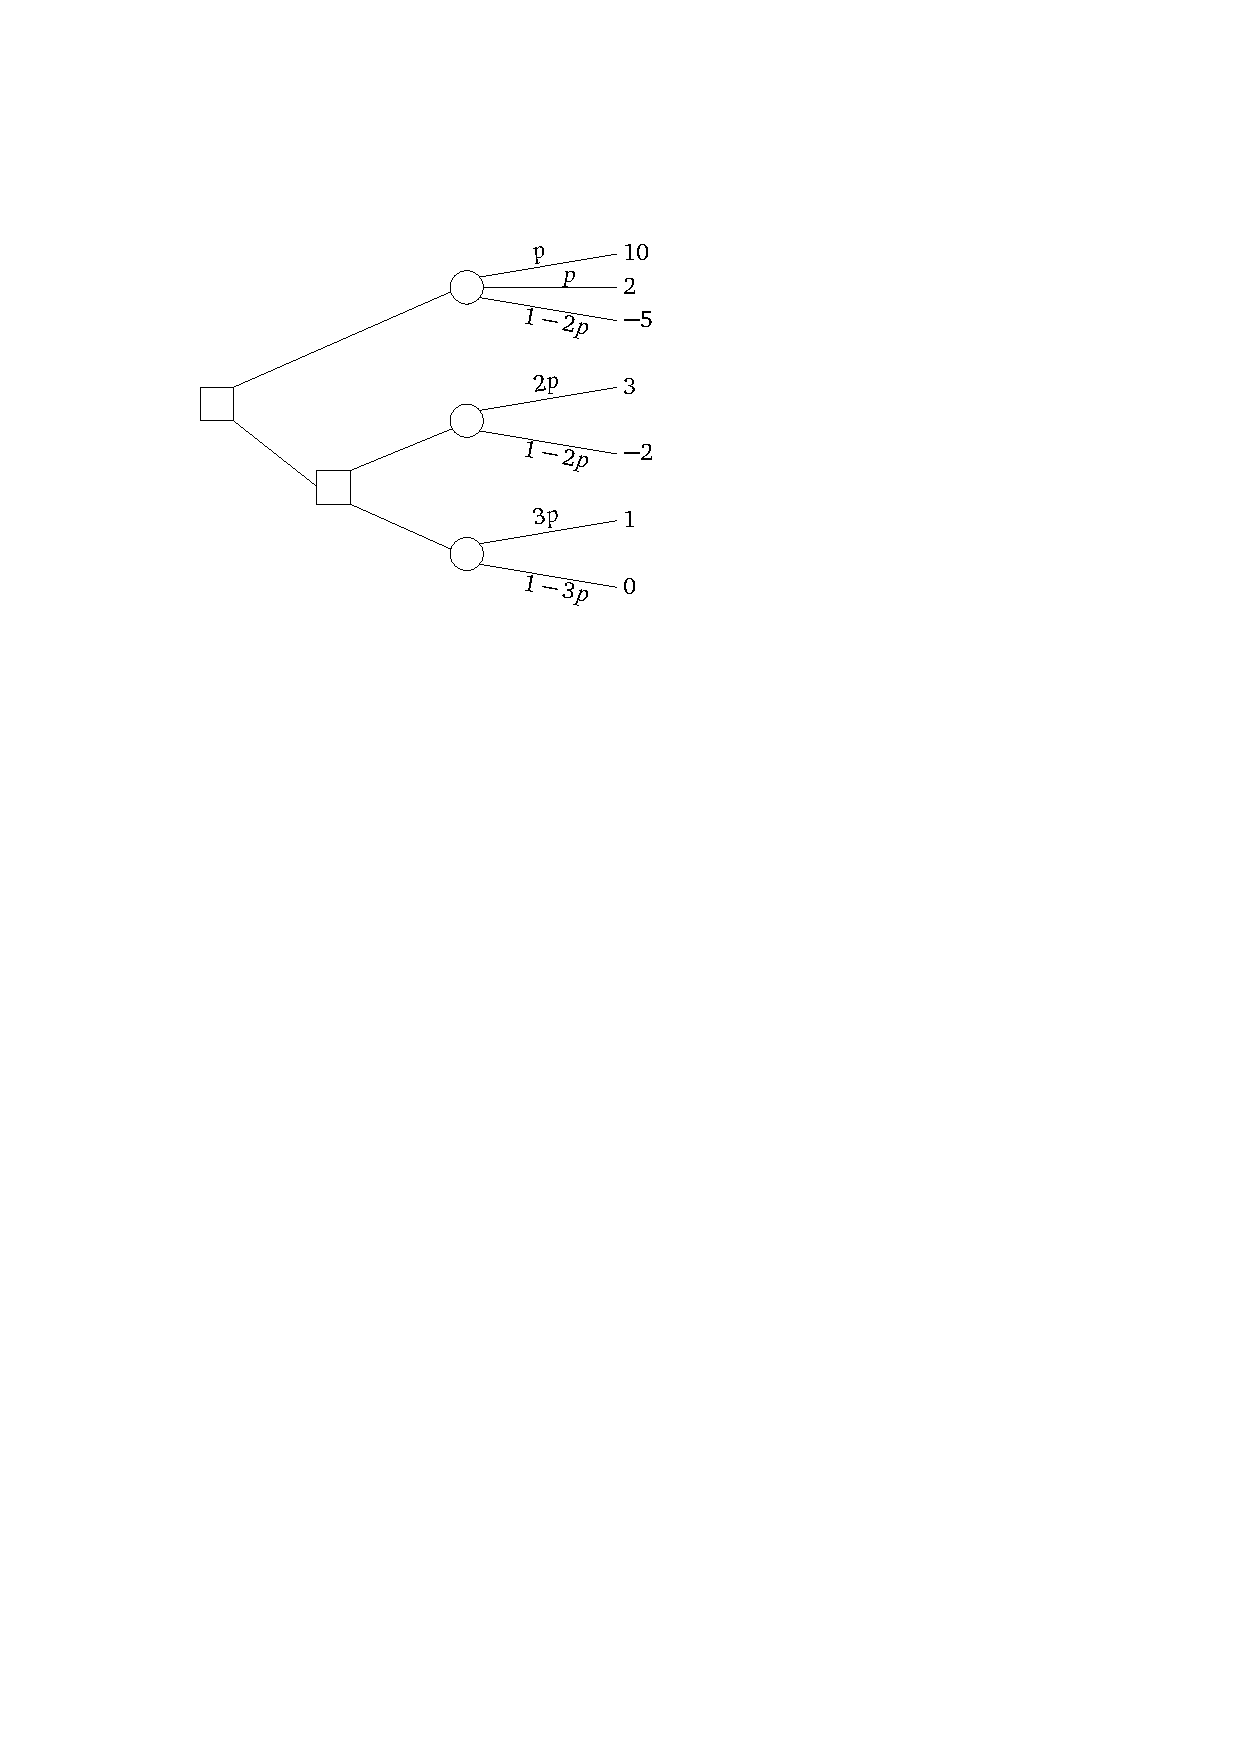
\includegraphics{slike/decision-tree.pdf}
\podnaslov{Odločitveno drevo}
\end{slika}
\end{vprasanje}
\begin{odgovor}
\end{odgovor}
\end{naloga}


\begin{naloga}{Janoš Vidali}{Izpit OR 15.12.2016}
\begin{vprasanje}[avtobus]
Mudi se ti na izpit, a ravno v trenutku,
ko prideš na postajo Konzorcij, odpelje avtobus številka 1.
Na prikazovalniku se izpiše,
da bo naslednji avtobus številka 1 prispel čez $10$ minut,
naslednji avtobus številka 6 čez $6$ minut,
naslednji avtobus številka 14 pa čez $2$ minuti.

Avtobusa 1 in 6 ob ugodnih semaforjih potrebujeta $6$ minut do postaje pri FE,
pri čemer se lahko čas vož\-nje zaradi rdeče luči na semaforju pri FF
podaljša za $1$ minuto.
Verjetnosti, da bo rdečo luč imel avtobus 1, da bo rdečo luč imel avtobus 6,
ter da bosta oba avtobusa imela zeleno luč, so enake $1/3$
(zaradi majhnega razmaka se ne more zgoditi,
da bi oba avtobusa naletela na rdečo luč).
Avtobus številka 1 nadaljuje pot do postaje pri FMF,
za kar potrebuje še $2$ minuti.

Avtobus številka 14 potrebuje $5$ minut do postaje pri študentskih domovih,
od tam pa greš peš do postaje pri FE, za kar potrebuješ še $4$ minute.
Pri tem prečkaš že\-lez\-ni\-co -- če mimo pripelje vlak
(kar se zgodi z verjetnostjo $0.05$),
se čas hoje podaljša za $3$ minute.
Ko prideš na postajo pri FE
(ne glede na to, ali si prišel z avtobusom 6 ali 14),
te čakajo še $4$ minute hoje do FMF,
vendar moraš najprej prečkati Tržaško cesto.
Če je na semaforju rdeča luč
(kar se zgodi z verjetnostjo 0.9, neodvisno od drugih dogodkov),
se lahko odločiš, da $2$ minuti počakaš na zeleno luč in potem nadaljuješ peš,
ali pa da greš nazaj do postaje in počakaš na avtobus številka $1$
(ki bo, tako kot prej, vozil še $2$ minuti do FMF).

Kakšne bodo tvoje odločitve,
da bo pričakovano trajanje poti do FMF čim krajše?
Nariši od\-lo\-čit\-ve\-no drevo
in odločitve sprejmi na podlagi izračunanih verjetnosti!
Glej sliko~\fig{} za shemo možnih poti.

\begin{slika}
\pgfslika
\podnaslov{Shema možnih poti}
\end{slika}
\end{vprasanje}
\begin{odgovor}
\end{odgovor}
\end{naloga}


\begin{naloga}{Janoš Vidali}{Izpit OR 31.1.2017}
\begin{vprasanje}
Dve podjetji bosta predstavili konkurenčna izdelka.
Možnost imaš kupiti delnice prvega podjetja za ceno $10000 €$
ali delnice drugega podjetja po ceni $5000 €$,
lahko pa se seveda odločiš tudi, da delnic ne kupiš.
Ocenjuješ, da bo z verjetnostjo $0.4$ uspelo prvo podjetje,
z verjetnostjo $0.1$ bo uspelo drugo podjetje,
z verjetnostjo $0.5$ pa ne bo uspelo nobeno izmed njiju
(ne more se zgoditi, da bi obe uspeli).
Ob uspehu prvega podjetja se bo vrednost njihovih delnic potrojila,
ob uspehu drugega podjetja pa se bo vrednost njihovih delnic popeterila
-- če si lastiš delnice uspešnega podjetja, jih torej lahko prodaš,
pri čemer bo torej dobiček enak
dvakratniku oziroma štirikratniku vloženega zneska.
Delnic neuspešnega podjetja ne bo želel nihče kupiti,
tako da je v tem primeru vloženi znesek izgubljen.

Za mnenje lahko povprašaš tržnega izvedenca,
ki bo po opravljeni raziskavi povedal,
katero od dveh podjetij ima večje možnosti za uspeh.
Če bo uspešno prvo podjetje, bo to pravilno napovedal z verjetnostjo $0.8$,
če pa bo uspešno drugo podjetje,
bo to pravilno napovedal z verjetnostjo $0.7$.
V primeru, ko podjetji ne bosta uspeli,
bo z verjetnostjo $0.4$ večje možnosti pripisal prvemu,
z verjetnostjo $0.6$ pa drugemu podjetju.
Za svoje mnenje izvedenec računa $1000 €$.

Kakšne bodo tvoje odločitve,
da bo tvoj pričakovani dobiček po odprodaji delnic čim večji?
Nariši od\-lo\-čit\-ve\-no drevo
in odločitve sprejmi na podlagi izračunanih verjetnosti.
Pričakovani dobiček tudi izračunaj.
\end{vprasanje}
\begin{odgovor}
\end{odgovor}
\end{naloga}


\begin{naloga}{Janoš Vidali}{Izpit OR 10.7.2017}
\begin{vprasanje}
Proti računalniškemu programu igraš Texas hold 'em poker.
Pravila igre tukaj niso pomembna.
Ker imaš dostop do kode programa, poznaš logiko, po kateri se ravna.
V trenutni igri si vložil $30$ žetonov, enako tudi nasprotnik.
Nasprotnik z verjetnostjo $0.6$ meni, da so odprte karte ugodnejše zate,
z verjetnostjo $0.4$ pa, da so ugodnejše zanj
(sam si ne ustvariš nobenega mnenja).
V prvem primeru je verjetnost, da so dejansko tvoje karte boljše, enaka $0.8$,
v drugem pa le $0.1$.

Nasprotnik se bo sedaj odločil, ali naj vloži še $10$ žetonov.
Sam se lahko nato odločiš, ali boš vložil $0$, $10$ ali $20$ žetonov
(skupni vložek bo torej $30$, $40$ ali $50$ žetonov).
Če je tvoj vložek manjši od nasprotnikovega,
je igra izgubljena in izgubiš do sedaj vloženo.
Če je tvoj vložek enak na\-sprot\-ni\-ko\-ve\-mu,
z nasprotnikom pogledata karte in tako določita zmagovalca.
Če je tvoj vložek višji od nasprotnikovega,
ima ta možnost odstopiti (tako pridobiš nasprotnikov vložek),
ali pa izenačiti, nakar se zmagovalec določi na podlagi kart.
Če zmagaš, pridobiš nasprotnikov vložek,
če izgubiš, pa izgubiš svojega.

V spodnji tabeli so zbrane verjetnosti dogodkov
v odvisnosti od nasprotnikovega mnenja glede kart.
Verjetnosti navedenih dogodkov pri istem mnenju so med seboj neodvisne.
\begin{center}
\makebox[\textwidth][c]{
\begin{small}
\begin{tabular}{r|cc}
dogodek $\setminus$ nasprotnikovo mnenje
& ugodnejše karte zate & za nasprotnika \\ \hline
dejansko imaš boljše karte & 0.8 & 0.1 \\
nasprotnik vloži $10$ žetonov po razkritju karte & 0.3 & 0.8 \\
nasprotnik izenači skupni vložek $40$ žetonov & 0.2 & 0.7 \\
nasprotnik izenači skupni vložek $50$ žetonov & 0.1 & 0.8
\end{tabular}
\end{small}
}
\end{center}
Na primer:
\begin{multline*}
\Pr[\text{nasprotnik izenači skupni vložek $40$ žetonov} \ | \\
| \ \text{nasprotnikovo mnenje je ``ugodnejše karte zate''}] = 0.2 .
\end{multline*}

Kakšne bodo tvoje odločitve,
da bo tvoj pričakovani dobiček po koncu igre čim večji?
Nariši odločitveno drevo
in odločitve sprejmi na podlagi izračunanih verjetnosti.
Pričakovani dobiček tudi izračunaj.
\end{vprasanje}
\begin{odgovor}
\end{odgovor}
\end{naloga}


\begin{naloga}{Janoš Vidali}{Izpit OR 29.8.2017}
\begin{vprasanje}[dectree2]
Dano je odločitveno drevo s slike~\fig{},
pri čemer velja $0 \le p \le 1/4$.
Pričakovano vred\-nost želimo maksimizirati.
Poišči optimalne odločitve in pričakovano vrednost
v odvisnosti od vrednosti parametra $p$.

\begin{slika}
\pgfslika
\podnaslov{Odločitveno drevo}
\end{slika}
\end{vprasanje}
\begin{odgovor}
\end{odgovor}
\end{naloga}


\begin{naloga}{Janoš Vidali}{Kolokvij OR 23.4.2018}
\begin{vprasanje}
Mladi podjetnik je razvil inovativen izdelek
in se odloča za nadaljnje korake pri njegovem trženju.
Naenkrat lahko naroči izdelavo $500$ izdelkov po ceni $10000 €$
ali $1000$ izdelkov po ceni $18000 €$,
lahko se pa odloči tudi, da izdelave ne naroči.
Podjetnik ocenjuje, da je izdelek tržno zanimiv z verjetnostjo $0.8$.
Odloča se, ali naj posamezen izdelek prodaja po ceni $50 €$ ali $60 €$,
pri čemer so v spodnji tabeli zbrana pričakovana števila prodanih kosov
v odvisnosti od teh pogojev.

\begin{center}
\begin{tabular}{c|cc}
& cena $50 €$ & cena $60 €$ \\
\hline
tržno zanimiv & $650$ & $550$ \\
tržno nezanimiv & $250$ & $100$ \\
\end{tabular}
\end{center}

Predpostavi, da se bodo prodali vsi izdelani kosi,
če je število teh manjše od pričakovane prodaje pri danih pogojih.

\begin{enumerate}[(a)]
\item Kako naj se podjetnik odloči, da bo pričakovani zaslužek čim večji?
Nariši od\-lo\-čit\-ve\-no drevo in ga uporabi pri sprejemanju odločitev.

\item V zadnjem trenutku je podjetnik izvedel,
da bo Podjetniški pospeševalnik objavil
razpis za nagrado za najboljši izdelek.
Razpisni pogoji zahtevajo,
da se za potrebo kontrole kvalitete izdela vsaj $1000$ izdelkov,
od katerih komisija izbere $20$ za dejansko kontrolo,
z ostalimi pa lahko prijavitelj prosto razpolaga.
Če podjetnik zmaga, bo dobil nagrado v višini $k$ evrov,
pri čemer $k \in [1000, 5000]$ še ni znan,
poleg tega pa si obeta tudi $20\%$ povečanje
pričakovanega števila prodanih kosov (v vseh zgoraj omenjenih pogojih).
Če ne zmaga, se pričakovanja ne spremenijo.
Podjetnik ocenjuje, da je verjetnost zmage enaka $0.6$,
če je izdelek tržno zanimiv,
in $0.1$, če izdelek ni tržno zanimiv.

Naj se podjetnik prijavi na razpis?
Nariši odločitveno drevo in odločitve sprejmi v odvisnosti od parametra $k$!
\end{enumerate}
\end{vprasanje}
\begin{odgovor}
\end{odgovor}
\end{naloga}


\begin{naloga}{Janoš Vidali}{Izpit OR 11.6.2018}
\begin{vprasanje}[vrac]
Podajamo se na pot v mesto na drugi strani gorovja.
Lahko se odločimo za pot po cesti okoli gorovja,
za kar bomo porabili $12$ ur.
Vendar pa nas najkrajša pot vodi čez prelaz,
ki je eno uro stran od začetne lokacije.
Žal pa so razmere v gorah nepredvidljive:
ocenjujemo, da bo z verjetnostjo $0.2$ prelaz čist
in ga bomo lahko prevozili v $5$ urah,
z ve\-rjet\-nost\-jo $0.1$ bo delno zasnežen in ga bomo prevozili v $9$ urah,
z verjetnostjo $0.7$ pa bo neprevozen,
zaradi česar se bomo morali vrniti na začetek in iti okoli gorovja
(skupno trajanje poti bo v tem primeru torej $14$ ur).

Edini, ki nam lahko kakorkoli pomaga pri oceni vremenskih razmer na prelazu,
je lokalni vrač,
ki pa živi v dolini pod goro in ne uporablja sodobne tehnologije,
s katero bi ga lahko kontaktirali.
Rade volje pa nam bo povedal, ali na gori vlada mir,
če se na poti do prelaza ustavimo pri njem.
Pogojne verjetnosti njegovega odgovora v odvisnosti od razmer na prelazu
so podane v spodnji tabeli.
\begin{center}
\makebox[\textwidth][c]{
\begin{tabular}{c|ccc}
$P\left(\text{vračev odgovor} \;\middle|\; \text{razmere na prelazu}\right)$
& čist & delno zasnežen & neprevozen \\ \hline
na gori vlada mir & $0.9$ & $0.5$ & $0.1$ \\
na gori divja vojna & $0.1$ & $0.5$ & $0.9$
\end{tabular}
}
\end{center}
Do vrača imamo eno uro vožnje, do prelaza pa potem še eno uro.
Če se po obisku vrača odločimo za pot okoli gorovja,
bomo za nadaljnjo pot porabili $12$ ur.

Kako se bomo odločili?
Nariši odločitveno drevo in ga uporabi pri sprejemanju odločitev.
Izračunaj tudi pričakovano trajanje poti.
Glej sliko~\fig{} za shemo možnih poti.

\begin{slika}
\pgfslika
\podnaslov{Shema možnih poti}
\end{slika}
\end{vprasanje}
\begin{odgovor}
\end{odgovor}
\end{naloga}


\begin{naloga}{Janoš Vidali}{Izpit OR 28.8.2018}
\begin{vprasanje}[dectree3]
Dano je odločitveno drevo s slike~\fig{},
pri čemer velja $0 \le p \le 1$.
Pričakovano vred\-nost želimo maksimizirati.
Poišči optimalne odločitve in pričakovano vrednost
v odvisnosti od vrednosti parametra $p$.

\begin{slika}
\pgfslika
\podnaslov{Odločitveno drevo}
\end{slika}
\end{vprasanje}
\begin{odgovor}
\end{odgovor}
\end{naloga}


\begin{naloga}{?}{Kolokvij OR 26.1.2010}
\begin{vprasanje}[ajkalaj]
V ugledni banki nameravajo okrepiti upravni odbor
z direktorjem za informacijske tehnologije.
Za svetovanje in pridobivanje kandidatov za to mesto
so prosili znano agencijo za kadrovsko svetovanje {\em Kadria d.o.o.}
Ti so jim priporočili prodornega g.~Miho Ajkalaja.
Po intervjuju z g.~Ajkalajem je direktor ocenil,
da bo g.~Ajkalaj z verjetnostjo $p = 3/5$ v enem letu uspešen pri svojem delu.
Če bo uspešen, bo banka dodatno prislužila $2.100.000 €$,
sicer pa bo pridelala dodatno izgubo $800.000 €$
(izobraževanje, vpeljava, odpravnina, \dots).

\begin{enumerate}[(a)]
\item Modeliraj problem v okviru teorije odločanja (stanja, odločitve).
Kakšno odločitev svetuješ direktorju glede na pričakovni dobiček?
Kako je odločitev odvisna od verjetnosti $p$?
Nariši graf, ki prikazuje optimalni pričakovani dobiček v odvisnosti od $p$.

\item Za dodatnih $80.000 €$ lahko agencija
z g.~Ajkalajem opravi dodatne inteligenčne in psihološke teste,
s katerimi lahko ugotovi, ali bo g.~Ajkalaj uspešen.
Statistični povzetek uspešnosti metode v preteklosti je naslednji:
\begin{center}
\begin{tabular}{l|cc}
$P(\text{izid testa} \;|\; \text{posl.~rezultat})$ &
\multicolumn{2}{c}{Izid testa} \\
Poslovni rezultat & pozitiven & negativen \\ \hline
uspešen   &  $7/8$ & $1/8$ \\
neuspešen &  $1/4$ & $3/4$
\end{tabular}
\end{center}
Izračunaj $\EVPI$ in $\EVE$ ter komentiraj,
ali je smiselno izvesti dodatna testiranja.

\item Nariši drevo odločitev in ugotovi,
ali naj direktor izvede testiranje in če ga,
kako naj se odloči glede zaposlitve g.~Ajkalaja.
\end{enumerate}
\end{vprasanje}

\begin{odgovor}
\begin{enumerate}[(a)]
\item Imamo eno odločitev -- ali naj zaposlimo g.~Ajkalaja.
Če ga ne zaposlimo, je dobiček $0 €$,
če pa ga zaposlimo, pa pridemo v stanje,
v katerem imamo z verjetnostjo $p$ dobiček $2.100.000 €$,
z verjetnostjo $1-p$ pa $-800.000 €$.
V tem stanju je torej pričakovan dobiček enak
$$
p \cdot 2.100.000 € - (1-p) \cdot 800.000 € =
p \cdot 2.900.000 € - 800.000 € .
$$
Za $p < 8/29$ torej pričakujemo izgubo in se nam ga ne izplača zaposliti,
sicer pa imamo dobiček in se ga nam tako izplača zaposliti.
Graf pričakovanega dobička je prikazan na sliki~\fig{ajkalaj-graf}.
Pri podani vrednosti $p = 3/5$ se nam torej izplača zaposliti g.~Ajkalaja,
saj tedaj pričakujemo dobiček $940.000 €$.

\item $\EVPI$ izračunamo tako,
da od pričakovanega dobička pri znanem izidu
odštejemo pričakovani dobiček pri neznanem izidu:
$$
\EVPI = 3/5 \cdot 2.100.000 € + 2/5 \cdot 0€ - 940.000 € = 320.000 €
$$
Ker je $\EVPI$ večji od cene dodatnega testiranja,
izračunajmo še $\EVE$.
Najprej določimo verjetnosti:
\begin{align*}
P(\text{test pozitiven}) = 7/8 \cdot 3/5 + 1/4 \cdot 2/5 &= 5/8 \\
P(\text{test negativen}) = 1/8 \cdot 3/5 + 3/4 \cdot 2/5 &= 3/8 \\
P(\text{uspešen rezultat} \;|\; \text{test pozitiven}) =
{7/8 \cdot 3/5 \over 5/8} &= 21/25 \\
P(\text{neuspešen rezultat} \;|\; \text{test pozitiven}) =
{1/4 \cdot 2/5 \over 5/8} &= 4/25 \\
P(\text{uspešen rezultat} \;|\; \text{test negativen}) =
{1/8 \cdot 3/5 \over 3/8} &= 1/5 \\
P(\text{neuspešen rezultat} \;|\; \text{test negativen}) =
{3/4 \cdot 2/5 \over 3/8} &= 4/5
\end{align*}
Sedaj lahko izračunamo $\EVE$:
\begin{multline*}
\EVE = (21/25 \cdot 2.100.000 € - 4/25 \cdot 800.000 €) \cdot 5/8 \, + \\
(1/5 \cdot 0 € + 4/5 \cdot 0 €) \cdot 3/8 - 940.000 € = 82.500 €
\end{multline*}
Ker je $\EVE$ večji od cene testiranja, se torej odločimo za testiranje.

\item Odločitveno drevo je prikazano na sliki~\fig{ajkalaj-drevo}.
Odločimo se za test -- če je ta pozitiven, zaposlimo g.~Ajkalaja, sicer pa ne.
\end{enumerate}

\begin{slika}
\pgfslika[ajkalaj-graf]
\podnaslov[\res{}(a)]{Graf pričakovanega dobička}
\end{slika}

\begin{slika}
\makebox[\textwidth][c]{
\pgfslika[ajkalaj-drevo]
}
\podnaslov[\res{}(c)]{Odločitveno drevo}
\end{slika}
\end{odgovor}
\end{naloga}


\begin{naloga}{?}{Izpit OR 28.6.2010}
\begin{vprasanje}[bp]
Na naftni ploščadi podjetja BP
je prišlo do nekontroliranih izpustov nafte iz vrtine v zalivu.
Po vseh mogočih podvigih, da bi zamašili vrtino,
se je ob\-upa\-no vodstvo podjetja pod pritiski predsednika bližnje države
začelo dobivati z ruskimi strokovnjaki
za mašenje vrtin s pomočjo jedrskih eksplozij pod vodstvom
prof.~dr.~Mikhaila Razturoviča Totalkova.
Vodstvo BP ocenjuje, da bo ekipa dr.~Totalkova
z verjetnostjo $p = 3/7$ uspešno zamašila vrtino.
Tako bo podjetje imelo sicer samo $2.8$ milijarde USD dobička,
sicer pa bi zaradi upada dobička in povzročene škode
utrpeli izgubo $700$ milijonov USD.

\begin{enumerate}[(a)]
\item Modeliraj problem v okviru teorije odločanja (stanja, odločitve).
Kakšno odločitev svetuješ vodstvu BP?
Kako je odločitev odvisna od verjetnosti $p$?
Nariši graf, ki prikazuje optimalni pričakovani dobiček v odvisnosti od $p$.

\item Za dodatnih $90.000$ USD lahko podjetje BP naroči študijo
pri kitajskem ljudskem inštitutu za naftne vrtine iz mesta Lanzhou,
ki ocenjuje uspešnost rizičnih projektov,
in bi ocenilo, ali bo ekipa dr.~Totalkov uspešna.
Statistični povzetek uspešnosti raziskav inštituta v preteklosti je naslednji:
\begin{center}
\begin{tabular}{l|cc}
$P(\text{rez.~raziskave} \;|\; \text{rez.~prov})$ &
\multicolumn{2}{c}{Rezultat raziskave inštituta} \\
Rezultat projekta & pozitiven & negativen \\ \hline
uspešen   &  $7/9$ & $2/9$ \\
neuspešen &  $1/3$ & $2/3$
\end{tabular}
\end{center}
Izračunaj $\EVPI$ in $\EVE$ ter komentiraj,
ali je smiselno izvesti dodatno raz\-iska\-vo.

\item Nariši drevo odločitev in ugotovi,
ali naj podjetje naroči raziskavo in če jo,
kako naj se odloči glede mašenja vrtine.
\end{enumerate}
\end{vprasanje}
\begin{odgovor}
\end{odgovor}
\end{naloga}


\begin{naloga}{?}{Izpit OR 15.9.2010}
\begin{vprasanje}
Letalska družba namerava nabaviti že rabljeno letalo, ki stane $170.000 €$.
Ocenjujejo, da bodo z njim imeli,
če je odlično ohranjeno, $1.000.000 €$ dobička,
če je zadovoljivo ohranjeno, $340.000 €$ dobička,
in če je slabo ohranjeno, le $10.000 €$ dobička.
Verjetnosti, da je letalo odlično, zadovoljivo ali slabo ohranjeno,
so zaporedoma $0.2$, $0.3$ in $0.5$.
\begin{enumerate}[(a)]
\item Modeliraj problem v okviru teorije odločanja (stanja, odločitve).
Kakšno odločitev svetuješ vodstvu družbe?

\item Družba lahko naroči oceno letala pri izvedenski firmi,
ki zahteva za svoje poročilo $10.000 €$.
Vodstvo družbe takole ocenjuje pogojne verjetnosti:
\begin{center}
\begin{tabular}{c|ccc}
$P(\text{rezultat poročila} \;|\;\ \text{kakovost letala})$
& odlično & zadovoljivo & slabo \\ \hline
ugodno & 0.9 & 0.6 & 0.1 \\
neugodno & 0.1 & 0.4 & 0.9
\end{tabular}
\end{center}
Kako naj se vodstvo družbe odloči?
\end{enumerate}

\end{vprasanje}
\begin{odgovor}
\end{odgovor}
\end{naloga}


\begin{naloga}{?}{Kolokvij OR 24.1.2011}
\begin{vprasanje}
Študent tretjega letnika finančne matematike se mora odločiti,
ali bi nadaljeval študij na drugi stopnji.
Ocenjuje, da bo, če študij uspešno zaključi,
v življenju zaslužil $200.000 €$ več,
kot če študij zaključi že po prvi stopnji.
Če pa študija ne zaključi uspešno,
bo imel zaradi stroškov študija in izgubljenega dohodka $40.000 €$ izgube.
Verjetnost, da bo študij na drugi stopnji uspešno zaključil, je $80 \%$.
\begin{enumerate}[(a)]
\item Modeliraj problem v okviru teorije odločanja (stanja, odločitve).
Kakšno odločitev svetuješ študentu?

\item Matematični oddelek ponuja dodatno testiranje,
ki študentom pomaga pri odločitvi, ali naj nadaljujejo študij.
Test stane $500$ evrov,
iz izkušenj kolegov pa študent ocenjuje,
da so pogojne verjetnosti naslednje:
\begin{center}
\begin{tabular}{c|cc}
$P(\text{rezultat testa} \;|\; \text{uspešnost študija})$
& uspešen & neuspešen \\ \hline
pozitiven & $19/20$ & $1/10$ \\
negativen & $1/20$ & $9/10$
\end{tabular}
\end{center}
Ali naj se študent prijavi na dodatno testiranje?
\end{enumerate}
\end{vprasanje}
\begin{odgovor}
\end{odgovor}
\end{naloga}


\begin{naloga}{?}{Izpit OR 9.2.2011}
\begin{vprasanje}
Direktorica banke se mora odločiti, ali bi stranki, računalniškemu podjetju,
odobrila posojilo v vrednosti $100.000 €$.
Po izkušnjah banke so računalniška podjetja neuspešna z verjetnostjo $20 \%$,
povprečno uspešna z verjetnostjo $50 \%$ in uspešna z verjetnostjo $30 \%$.
Če damo podjetju kredit in se izkaže za neuspešno,
bomo imeli v povprečju za $15.000 €$ izgube,
če je povprečno upešno, bomo imeli $10.000 €$ dobička,
če pa je uspešno, bomo imeli $20.000 €$ dobička.
\begin{enumerate}[(a)]
\item Modeliraj problem v okviru teorije odločanja (stanja, odločitve).
Kakšno odločitev svetuješ direktorici banke?
Kolikšen je EVPI?

\item Za ceno $5.000 €$ lahko najamemo podjetje,
ki natančno preuči računalniško podjetje in poda svojo oceno:
negativno, nevtralno ali pozitivno.
Po podatkih banke so pogojne verjetnosti
$P(\text{rezultat testa} \;|\; \text{uspešnost podjetja})$ naslednje:
\begin{center}
\begin{tabular}{c|ccc}
& neuspešno & povprečno uspešno & uspešno \\ \hline
negativno & $1/2$  & $2/5$  & $1/5$ \\
nevtralno & $2/5$  & $1/2$  & $2/5$ \\
pozitivno & $1/10$ & $1/10$ & $2/5$
\end{tabular}
\end{center}
Izračunaj EVE in nariši odločitveno drevo.
Kakšno odločitev svetuješ direktorici banke?
\end{enumerate}
\end{vprasanje}
\begin{odgovor}
\end{odgovor}
\end{naloga}


\begin{naloga}{?}{Vaje OR 11.4.2008}
\begin{vprasanje}
Janez želi naložiti vsoto $1000 €$ v banko za dobo petih let.
Odloča se med tem, da bi jo vezal za pet let (obrestna mera $5\%$)
ali pa petkrat zaporedoma po eno leto (obrestna mera $4\%$).
Če denar veže za pet let, vmes pa varčevanje prekine,
mu pripada le obrestna mera $3\%$.
Ocenjuje, da lahko v naslednjih petih letih pride do naslednjih situacij:
\begin{itemize}
\item varčeval bo pet let, pri tem se obrestna mera ne spremeni,
\item varčeval bo pet let, obrestna mera se po treh letih poveča za $30\%$,
\item varčeval bo pet let, obrestna mera se po treh letih zmanjša za $20\%$,
\item varčeval bo tri leta.
\end{itemize}
Opiši, kako naj se odloči glede na posamezne kriterije
(optimist, pesimist, Laplace, Savage).
Določi vrednosti parametera $\alpha$,
pri katerih je po Hurwiczevem kriteriju možnih več enakovrednih odločitev.
\end{vprasanje}

\begin{odgovor}
Zaradi enostavnosti predpostavimo,
da se obrestuje samo glavnica (enkrat na leto),
pri čemer pri petletnem varčevanju vsakič velja začetna obrestna mera.
Izračunajmo obresti po petih letih pri različnih shemah vezave
glede na dogajanje po treh letih:
\begin{center}
\begin{tabular}{c|cccc}
shema & nespremenjena & povečana & zmanjšana & prekinitev \\ \hline
$5$ let              & $250$ & $250$ & $250$ &   $-$ \\
$3 + 2 \cdot 1$ leto & $170$ & $194$ & $154$ &   $-$ \\
$3$ leta             &  $90$ &  $90$ &  $90$ &  $90$ \\ \hline
$5 \cdot 1$ leto     & $200$ & $224$ & $184$ &   $-$ \\
$3 \cdot 1$ leto     & $120$ & $120$ & $120$ & $120$ \\
\end{tabular}
\end{center}
Drugih možnosti ne bomo obravnavali,
saj se očitno $5$-letna vezava ne izplača, če jo bomo predčasno prekinili.
Iz zgornje tabele je torej jasno,
da se bomo odločili bodisi za $5$-letno vezavo ali pa vsakoletno vezavo,
z morebitno prekinitvijo oziroma prenehanjem po $3$ letih
brez nadaljnje vezave.
Dobimo torej sledečo odločitveno tabelo:
\begin{center}
\begin{tabular}{c|cccc}
začetna shema & nespremenjena & povečana & zmanjšana & prekinitev \\ \hline
$5$ let          & $250$ & $250$ & $250$ &  $90$ \\
$5 \cdot 1$ leto & $200$ & $224$ & $184$ & $120$ \\
\end{tabular}
\end{center}

Pri optimistovem kriteriju se ravnamo glede na najboljši možen izid.
Pri $5$-letni vezavi je to $250 €$, pri letni vezavi pa $224 €$,
zato se odločimo za $5$-letno vezavo.

Pri pesimistovem (Waldovem) kriteriju se ravnamo glede na najslabši možen izid.
Pri $5$-letni vezavi je to $90 €$, pri letni vezavi pa $120 €$,
zato se odločimo za letno vezavo.

Pri Laplaceovem kriteriju so vse možnosti enako verjetne.
Pri $5$-letni vezavi je torej pričakovani dobiček enak
$(250 € + 250 € + 250 € + 90 €)/4 = 210 €$,
pri letni vezavi pa $(200 € + 224 € + 184 € + 120 €)/4 = 182 €$,
zato se odločimo za $5$-letno vezavo.

Pri Savageovem kriteriju želimo minimizirati največje možno obžalovanje.
Pri $5$-letni vezavi je največje obžalovanje enako $120 € - 90 € = 30 €$,
pri letni vezavi pa $250 € - \min\{200€, 224€, 184€\} = 66 €$,
zato se odločimo za $5$-letno vezavo.

Pri Hurwiczevem kriteriju upoštevamo,
da se najboljši izid zgodi z ve\-rjet\-nost\-jo $\alpha$,
najslabši pa z verjetnostjo $1 - \alpha$.
Pri $5$-letni vezavi je torej pričakovan dobiček enak
$\alpha \cdot 250 € + (1 - \alpha) \cdot 90 € = \alpha \cdot 160 € + 90 €$,
pri letni vezavi pa
$\alpha \cdot 224 € + (1 - \alpha) \cdot 120 € = \alpha \cdot 104 € + 120 €$.
Pri vrednosti $\alpha = 15/28$ sta obe možnosti enakovredni.
Pri večjih vrednostih $\alpha$ se odločimo za $5$-letno vezavo,
pri manjših pa za letno vezavo.
\end{odgovor}
\end{naloga}


\begin{naloga}{?}{Kolokvij OR 17.4.2013}
\begin{vprasanje}
Na letalu je $100$ sedežev.
Dane so naslednje verjetnosti za število potnikov,
ki ne pridejo na vkrcanje,
pri čemer je $P(i)$ verjetnost, da natanko $i$ potnikov ne pride na vkrcanje:
$$
P(0) = 0.25, \quad P(1) = 0.5, \quad P(2) = 0.25 .
$$
\begin{enumerate}[(a)]
\item Koliko letalskih kart naj proda letalska družba,
če vsak prazen sedež na letalu prinese $100 €$ izgube,
vsak nezadovoljen potnik, ki ne dobi sedeža, pa $200 €$ izgube?

\item Za $200 €$ lahko izvedemo predhodno analizo,
ki nam napove število potnikov, ki jih ne bo na vkrcanju.
Zanesljivost analize je podana z verjetnostmi
$$
(p_{ij})_{i,j=0}^2 = \begin{bmatrix}
0.7 & 0.1 & 0 \\
0.2 & 0.8 & 0.1 \\
0.1 & 0.1 & 0.9 \\
\end{bmatrix} ,
$$
kjer je $p_{ij}$ verjetnost,
da analiza napove odpoved $i$ potnikov v primeru,
ko imamo dejansko $j$ odpovedi.
Ali naj letalska družba izvede analizo pred prodajo kart?
\end{enumerate}
\end{vprasanje}
\begin{odgovor}
\end{odgovor}
\end{naloga}


\begin{naloga}{?}{Izpit OR 14.6.2013}
\begin{vprasanje}
Fenko, brat škrata Bolfenka, je najboljši alkimist, kar jih je družina imela.
Preživlja se z izdelovanjem zlata iz granodiorita\footnote{
Granodiorit je zelo razširjena magmatska kamnina na Pohorju,
znana tudi kot pohorski tonalit.
}.
Postopek izdelave zlata je naslednji:
ob 23:00 mora nastaviti sveže izkopan granodiorit
($1$ kg svežega granodiorita je vreden $2$ gulda\footnote{
Guld je denarna enota, ki jo uporabljajo pohorski škratje.
})
na točno določeno mesto pod milo nebo\footnote{
Kam je treba nastaviti granodiorit, je odvisno tudi od položaja planetov.
}.
Če nastavljene kamnine noben škrat, srna ali človek ne vidi,
se le-ta v dveh urah spremeni v zlato
(za $1$ kg granodiorita dobi $10$ g zlata).
Verjetnost, da se to zgodi (tj., da nastane zlato), je $2/5$.
To zlato lahko proda škratu zlatarju za gulde
(in to je edini možni način porabe zlata).
Za $10$ g zlata dobi $4$ gulde.
Granodiorit, ki je enkrat že bil nastavljen,
se ne bo nikoli več spremenil v zlato.
Fenko lahko kilogram ``porabljenega'' granodiorita proda za $1$ guld.

Predpostavimo, da Fenko zapravlja denar le za izdelavo zlata iz granodiorita,
da zmeraj nastavi celoštevilsko mnogo kilogramov granodiorita
in ima zmeraj celoštevilsko mnogo guldov
(npr.~s tremi guldi lahko kupi največ $1$ kg granodiorita, en guld mu ostane).

Trenutno ima Fenko $5$ guldov, nič zlata in nič granodiorita.
Koliko kilogramov granodiorita
naj v naslednjih dveh nočeh nastavi pod milo nebo,
da bo imel kar največje pričakovano število guldov?
V odgovoru napiši,
koliko granodiorita naj nastavi prvo noč in koliko drugo noč.
Odgovor bo odvisen od tega,
ali se mu ponoči granodiorit spremeni v zlato ali ne.
\end{vprasanje}
\begin{odgovor}
\end{odgovor}
\end{naloga}


\begin{naloga}{Batagelj, Kaufman}{\cite[Naloga~4.3]{bk}}
\begin{vprasanje}
Ljubo prodaja časopise po centru Ljubljane.
Vsak dan se mora odločiti, koliko časopisov naj naroči.
Za vsak naročen časopis plača $0.8 €$, iztrži pa $1 €$.
Za neprodane časopise ne dobi povrnjenega denarja.
Vsak dan je verjetnost, da bo imel $i$ kupcev, enaka $p_i$,
kjer je $p_6 = 0.1$, $p_7 = 0.2$, $p_8 = 0.3$, $p_9 = 0.3$ in $p_{10} = 0.1$.
\begin{enumerate}[(a)]
\item Kakšno odločitev svetuješ Ljubu in zakaj?
\item Kolikšen zaslužek lahko pričakuje v mesecu,
ko časopis izide petindvajsetkrat?
\end{enumerate}
\end{vprasanje}
\begin{odgovor}
\end{odgovor}
\end{naloga}


\begin{naloga}{?}{Izpit OR 24.6.2014}
\begin{vprasanje}
Tovarna od dobavitelja dobi paket $10$ komponent $A$.
Tovarna sestavlja izdelke $B$,
kjer gre v vsak izdelek $B$ natanko ena komponenta $A$.
Dane so verjetnosti
$$
p_i = P(\text{med $10$ komponentami $A$ je natanko $i$ pokvarjenih}),
$$
kjer je $p_1 = 0.7$, $p_2 = 0.2$ in $p_3 = 0.1$.
Stroški pregleda posamezne komponente so $45 €$.
Stroški popravila izdelka $B$ zaradi vgrajene okvarjene komponente $A$
so enaki $350 €$.
\begin{enumerate}[(a)]
\item Denimo, da ima tovarna na izbiro samo dve možnosti.
Prva je, da pregleda vseh $10$ dobavljenih izdelkov.
Druga možnost pa je, da ne pregleda nobenega dobavljenega izdelka.
Katera odločitev tovarni povzroči manj stroškov?

\item Naj ima sedaj tovarna na voljo drugačni izbiri.
Prva je, da naključno izbere eno izmed $10$ komponent $A$,
jo pregleda in po potrebi zamenja,
ter gre nato direktno v proizvajanje izdelkov $B$.
Druga možnost pa je, da pregleda vseh $10$ izdelkov.
Katera odločitev tovarni povzroči manj stroškov?
\end{enumerate}
\end{vprasanje}
\begin{odgovor}
\end{odgovor}
\end{naloga}


\begin{naloga}{?}{Izpit OR 25.8.2014}
\begin{vprasanje}
V škatli so štirje ponarejeni kovanci, vredni $0 €$,
in en zlat kovanec, vreden $100 €$.
Na slepo lahko izbereš po en kovanec,
pri čemer moraš za vsako izbiranje plačati $30 €$.
Določi povprečen profit, ki ga dosežeš pri igranju te igre.
\end{vprasanje}
\begin{odgovor}
\end{odgovor}
\end{naloga}


\begin{naloga}{?}{Izpit OR 12.5.2016}
\begin{vprasanje}
Smo v letu 2500 in turistične rakete že potujejo na Luno.
LunaAirways oglašuje let, na katerem je lahko $100$ potnikov.
LunaAirways računa, da bodo vsa mesta zasedena.
Z leti izkušenj vedo,
da nekatere potnike zagrabi strah in tako ne pridejo na potovanje.
Ocenjujejo, da je verjetnost $p_i$,
da natanko $i$ potnikov ($0 \le i \le 5$) ne pride na potovanje,
naslednje:
\begin{center}
\begin{tabular}{c|cc}
$i$ & od $0$ do $3$ & od $4$ do $5$ \\ \hline
$p_i$ & $0.2$ & $0.1$
\end{tabular}
\end{center}

S prodajo karte ima družba $300$ denot dobička.
Za vsakega potnika, ki bo moral menjati let,
ima LunaAirways $400$ denot stroškov.
Koliko kart naj proda LunaAirways, če želi maksimizirati pričakovani dobiček?
\end{vprasanje}
\begin{odgovor}
\end{odgovor}
\end{naloga}


\begin{naloga}{?}{Izpit OR 24.5.2016}
\begin{vprasanje}
Kavarna {\em ma$\phi$ja} je razvila recept za novo torto.
Slaščičarna {\em sladkeoperacijskeraziskave}
je za eksluzivno pravico do recepta pripravljena plačati $15002 €$.
Če se kavarna {\em ma$\phi$ja} odloči za samostojno prodajo torte,
jih začetni vložek stane $10000 €$,
za vsako prodano torto pa zaslužijo $25 €$.
Po njihovi presoji
je verjetnost uspeha recepture (prodajo $100000$ tort) enaka $0.4$,
verjetnost propada (prodali bi zgolj $10000$ tort) pa $0.6$.
Kavarna se lahko odloči, da zaprosi za pomoč tudi pod\-jet\-je,
ki na osnovi degustacij torte sestavi mnenje o uspehu recepta.
Svetovanje jih stane $35000 €$,
natančnost svetovanja pa opisuje spodnja tabela.
\begin{center}
\begin{tabular}{c|cc}
$P(\text{mnenje svetovalca} \;|\;\ \text{uspeh recepta})$
& Recept uspe & Recept ne uspe \\ \hline
Ugodno   & ${3 \over 4}$ & ${1 \over 2}$ \\
Neugodno & ${1 \over 4}$ & ${1 \over 2}$
\end{tabular}
\end{center}
Kako naj se kavarna {\em ma$\phi$ja} odloči?
Zakaj?
\end{vprasanje}
\begin{odgovor}
\end{odgovor}
\end{naloga}


\begin{naloga}{?}{Izpit OR 24.5.2016}
\begin{vprasanje}
Organizatorji olimpijskih iger so zgradili dvorano za judo,
ki sprejme $1000$ ljudi.
Popularnost juda je na vrhuncu,
zato organizatorji pričakujejo, da bodo vse karte zakupljene.
Zaradi straha pred virusom zika so analitiki
za $0 \le i \le 5$ ($i \in \Z$) izračunali verjetnosti $p_i$,
da se natanko $i$ izmed imetnikov kart ne pojavi na prireditvi.
Verjetnosti so zbrane v spodnji tabeli.
\begin{center}
\begin{tabular}{c|cccccc}
$i$   & $0$    & $1$    & $2$   & $3$   & $4$    & $5$ \\ \hline
$p_i$ & $0.01$ & $0.19$ & $0.3$ & $0.4$ & $0.05$ & $0.05$
\end{tabular}
\end{center}

S prodajo vstopnice imajo organizatorji $1000$ denot dobička.
Za vsakega obiskovalca,
ki bo ostal brez sedeža in bo moral v VIP sekcijo dvorane,
imajo $1400$ denot stroškov.
Koliko kart naj organizatorji olimpijskih iger prodajo,
če želijo maksimizirati pričakovani dobiček?
\end{vprasanje}
\begin{odgovor}
\end{odgovor}
\end{naloga}

\subsection{Dinamično programiranje}

\begin{naloga}{?}{Vaje OR 6.4.2016}
\begin{vprasanje}
Na avtocestni odsek dolžine $M$ kilometrov
želimo postaviti oglasne plakate.
Dovoljene lokacije plakatov določa urad za oglaševanje
in so predstavljene s števili $x_1, x_2, \dots x_n$,
kjer $x_i$ ($1 \le i \le n$)
predstavlja oddaljenost od začetka odseka v kilometrih.
Profitabilnost oglasa na lokaciji $x_i$ določa vrednost $v_i$
($1 \le i \le n$).
Urad za oglaševanje podaja tudi omejitev,
da mora biti razdalja med oglasi vsaj $d$ kilometrov.
Oglase želimo postaviti tako, da bodo čim bolj profitabilni.
\begin{enumerate}[(a)]
\item Reši problem za parametre $M = 20$, $d = 5$, $n = 8$,
$(x_i)_{i=1}^n = (1, 2, 8, 10, 12,$ $14, 17, 20)$ in
$(v_i)_{i=1}^n = (8, 8, 12, 10, 7, 5, 6, 10)$.
\item Napiši rekurzivne enačbe za opisani problem.
\item Napiši algoritem,
ki poišče najbolj profitabilno postavitev oglasov za dane parametre.
Kakšna je njegova časovna zahtevnost?
\end{enumerate}

\end{vprasanje}
\begin{odgovor}
\end{odgovor}
\end{naloga}


\begin{naloga}{?}{Vaje OR 6.4.2016}
\begin{vprasanje}
Imamo nahrbtnik nosilnosti $M$ kilogramov.
Danih je $n$ objektov z vrednostmi $v_i$ in težami $t_i$ ($1 \le i \le n$).
Problem nahrbtnika sprašuje po izbiri predmetov
$I \subseteq \{1, 2, \dots, n\}$,
ki maksimizira njihovo skupno vrednost pri omejitvi $\sum_{i \in I} t_i \le M$.
\begin{enumerate}[(a)]
\item Napiši rekurzivne enačbe za opisani problem.
\item Z uporabo rekurzivnih enačb reši problem za parametre $M = 8$, $n = 8$,
$(v_i)_{i=1}^n = (9, 9, 8, 11, 10, 15,$ $3, 12)$ in
$(t_i)_{i=1}^n = (3, 5, 1, 4, 3, 8, 2, 7)$.
\end{enumerate}

\end{vprasanje}
\begin{odgovor}
\end{odgovor}
\end{naloga}


\begin{naloga}{?}{Vaje OR 6.4.2016}
\begin{vprasanje}
Dana je matrika $A = (a_{ij})_{i,j=1}^{m,n}$.
Poiskati želimo pot minimalne vsote,
ki se začne v levem zgornjem kotu (pri $a_{11}$)
in konča v desnem spodnjem kotu (pri $a_{mn}$).
Dovoljeni so zgolj premiki v desno in navzdol.
\begin{enumerate}[(a)]
\item Reši problem za matriko
$$
A = \begin{pmatrix}
131 & 673 & 234 & 103 &  18 \\
201 &  96 & 342 & 965 & 150 \\
630 & 803 & 746 & 422 & 111 \\
537 & 699 & 497 & 121 & 956 \\
805 & 732 & 524 &  37 & 332
\end{pmatrix} .
$$
\item Napiši rekurzivne enačbe za opisani problem.
\item Na osnovi rekurzivnih enačb napiši algoritem, ki reši opisani problem.
Oceni tudi njegovo časovno zahtevnost v odvisnosti od $m$ in $n$.
\end{enumerate}

\end{vprasanje}
\begin{odgovor}
\end{odgovor}
\end{naloga}


\begin{naloga}{?}{Vaje OR 6.4.2016}
\begin{vprasanje}
Dan je niz $S = a_1 a_2 \dots a_n$,
kjer so $a_i$ ($1 \le i \le n$) elementi neke končne abecede.
Nizu $a_j a_{j+1} \dots a_k$, kjer je $1 \le j \le k \le n$,
pravimo {\em strnjen podniz} niza $S$.
S pomočjo dinamičnega programiranja napiši algoritem,
ki določi najdaljši palindromski strnjen podniz v $S$.

\end{vprasanje}
\begin{odgovor}
\end{odgovor}
\end{naloga}


\begin{naloga}{?}{Vaje OR 6.4.2016}
\begin{vprasanje}
Dana je matrika $A = (a_{ij})_{i,j=1}^{m,n}$.
Poiskati želimo strnjeno podmatriko matrike $A$
z največjo vsoto komponent.
\begin{enumerate}[(a)]
\item Reši problem za matriko
$$
A = \begin{pmatrix}
 1 & -1 &  2 &  4 \\
-3 & -2 &  8 &  2 \\
-3 &  2 & -2 &  4 \\
 1 & -5 & -1 & -2
\end{pmatrix} .
$$
\item Napiši rekurzivne enačbe za opisani problem.
\item Napiši algoritem, ki reši opisani problem.
Oceni tudi njegovo časovno zahtevnost v odvisnosti od $m$ in $n$.
\end{enumerate}

\end{vprasanje}
\begin{odgovor}
\end{odgovor}
\end{naloga}


\begin{naloga}{?}{Vaje OR 6.4.2016}
\begin{vprasanje}
Na voljo imamo kovance z vrednostmi $1 = v_1 < v_2 < \cdots < v_n$
in vsoto $C$, ki jo želimo izplačati s kovanci.
Predpostavljamo, da imamo dovolj velik nabor kovancev.
\begin{enumerate}[(a)]
\item Poišči izplačilo z najmanjšim številom kovancev
za $C = 25$, $n = 4$ in $(v_i)_{i=1}^n = (1, 2, 5, 7)$.
\item S pomočjo dinamičnega programiranja reši problem v splošnem.
\end{enumerate}

\end{vprasanje}
\begin{odgovor}
\end{odgovor}
\end{naloga}


\begin{naloga}{?}{Vaje OR 6.4.2016}
\begin{vprasanje}
Na ulici je $n$ vrstnih hiš,
pri čemer je v $i$-ti hiši $c_i$ denarja.
Tat se odloča, katere izmed hiš naj oropa.
Vsak oropan stanovalec to sporoči svojim sosedom,
zato tat ne sme oropati dveh sosednjih hiš.
Ker je tat poslušal predmet Operacijske raziskave,
pozna dinamično programiranje.
Pokaži, kako naj tat določi, katere hiše naj oropa.

\end{vprasanje}
\begin{odgovor}
\end{odgovor}
\end{naloga}


\begin{naloga}{?}{Kolokvij OR 31.5.2012}
\begin{vprasanje}
Imamo hlod dolžine $\ell$,
ki bi ga radi razžagali na $n$ označenih mestih
$0 < x_1 < x_2 < \dots < x_n < \ell$.
Eno rezanje stane toliko, kolikor je dolžina hloda, ki ga režemo.
Ko hlod prerežemo, dobimo dva manjša hloda, ki ju režemo naprej.
Poiskati želimo zaporedje rezanj z najmanjšo ceno.
\begin{enumerate}[(a)]
\item Reši problem pri podatkih $\ell = 10$ in $(x)_{i=1}^4 = (3, 5, 7, 8)$.
\item S pomočjo dinamičnega programiranja reši problem v splošnem.
Oceni tudi njegovo časovno zahtevnost.
\end{enumerate}

\end{vprasanje}
\begin{odgovor}
\end{odgovor}
\end{naloga}


\begin{naloga}{Hillier, Lieberman}{\cite[Problem~11.3-1]{hl}}
\begin{vprasanje}
Lastnik verige $n$ trgovin z živili je kupil $m$ zabojev svežih jagod.
Naj bo $p_{ij}$ pričakovan dobiček v trgovini $j$,
če tja dostavimo $i$ zabojev.
Zanima nas, koliko zabojev naj gre v vsako trgovino,
da bomo imeli čim večji zaslužek.
Zaradi logističnih razlogov zabojev ne želimo deliti.
\begin{enumerate}[(a)]
\item Z dinamičnim programiranjem reši problem za podatke $m = 5$, $n = 3$
in $p_{ij}$ iz sledeče tabele:
$$
\begin{array}{c|ccc}
p_{ij} & 1 & 2 & 3 \\
\hline
0 &  0 &  0 &  0 \\
1 &  5 &  6 &  4 \\
2 &  9 & 11 &  9 \\
3 & 14 & 15 & 13 \\
4 & 17 & 19 & 18 \\
5 & 21 & 22 & 20 \\
\end{array}
$$
\item Napiši algoritem, ki reši opisani problem v splošnem.
\end{enumerate}

\end{vprasanje}
\begin{odgovor}
\end{odgovor}
\end{naloga}


\begin{naloga}{Hillier, Lieberman}{\cite[Problem~11.3-8]{hl}}
\begin{vprasanje}
Podjetje bo kmalu uvedlo nov izdelek na zelo konkurenčen trg,
zato trenutno pripravlja marketinško strategijo.
Odločili so se, da bodo izdelek uvedli v treh fazah.
V prvi fazi bodo pripravili posebno začetno ponudbo z močno znižano ceno,
da bi privabili zgodnje kupce.
Druga faza bo vključevala intenzivno oglaševalsko kampanjo,
da bi zgodnje kupce prepričali, naj izdelek še vedno kupujejo po redni ceni.
Znano je, da bo ob koncu druge faze
konkurenčno podjetje predstavilo svoj izdelek.
Zato bo v tretji fazi okrepljeno oglaševanje z namenom,
da bi preprečili beg strank h konkurenci.

Podjetje ima za oglaševanje na voljo $4$ milijone evrov,
ki jih želimo čim bolj učinkovito porabiti.
Naj bo $m$ tržni delež v procentih, pridobljen v prvi fazi,
$f_2$ delež, ohranjen po drugi fazi,
in $f_3$ delež, ohranjen po tretji fazi.
Maksimizirati želimo končni tržni delež, torej količino $m f_2 f_3$.

\begin{enumerate}[(a)]
\item Denimo, da želimo v vsaki fazi porabiti nek večkratnik milijona evrov,
pri čemer bomo pri prvi fazi porabili vsaj milijon evrov.
V spodnji tabeli so zbrani vplivi porabljenih količin
na vrednosti $m$, $f_2$ in $f_3$.
$$
\begin{array}{c|ccc}
M€ & m & f_2 & f_3 \\
\hline
0 &  - & 0.2 & 0.3 \\
1 & 20 & 0.4 & 0.5 \\
2 & 30 & 0.5 & 0.6 \\
3 & 40 & 0.6 & 0.7 \\
4 & 50 &   - &   - \\
\end{array}
$$
Kako naj razdelimo sredstva?
\item Denimo sedaj,
da lahko v vsaki fazi porabimo poljubno pozitivno količino denarja
(seveda glede na omejitev skupne porabe).
Naj bodo torej $x_1$, $x_2$ in $x_3$ količine denarja v milijonih evrov,
ki jih porabimo v prvi, drugi in tretji fazi.
Vpliv na tržni delež je podan s formulami
$$
m = x_1 (10 - x_1), \quad
f_2 = 0.4 + 0.1 x_2, \quad \text{in} \quad
f_3 = 0.6 + 0.07 x_3 .
$$
Kako naj sedaj razdelimo sredstva?
\end{enumerate}

\end{vprasanje}
\begin{odgovor}
\end{odgovor}
\end{naloga}


\begin{naloga}{?}{Izpit OR 26.6.2012}
\begin{vprasanje}
Nori profesor Boltežar stanuje v stolpnici z $n$ nadstropji,
oštevilčenimi od $1$ do $n$.
Nori stanovalci tega bloka radi mečejo cvetlične lončke z balkonov.
Boltežar bi rad ugotovil, katero je najvišje nadstropje,
s katerega lahko pade cvetlični lonček, ne da bi se razbil.
Jasno je, da če se lonček razbije pri padcu iz $k$-tega nadstropja,
potem se razbije tudi pri padcu s $(k+1)$-tega nadstropja.
Če bi Boltežar imel le en cvetlični lonček,
bi ga lahko metal po vrsti od najnižjega nadstropja navzgor,
dokler se ne bi razbil.
V najslabšem primeru bi lonček torej vrgel $n$ krat
(možno je, da bi lonček preživel tudi padec iz najvišjega nadstropja).

Ker ima Boltežar doma $k$ cvetličnih lončkov,
lahko do rezultata pride tudi z manjšim številom metov.
S pomočjo dinamičnega programiranja bi rad poiskal strategijo metanja,
ki bi minimizirala število potrebnih metov v najslabšem primeru.
\begin{enumerate}[(a)]
\item Napiši rekurzivne enačbe za opisani problem.
\item Napiši algoritem, ki reši opisani problem.
Oceni tudi njegovo časovno zahtevnost v odvisnosti od $n$ in $k$.
\end{enumerate}

\end{vprasanje}
\begin{odgovor}
\end{odgovor}
\end{naloga}


\begin{naloga}{Hillier, Lieberman}{\cite[Problem~11.2-2]{hl}}
\begin{vprasanje}
Vodja prodaje pri založniku učbenikov za fakulteto
ima na voljo $6$ trgovskih potnikov,
ki jim želi dodeliti eno od treh regij, v kateri bodo delovali.
V vsaki regiji mora delovati vsaj en trgovski potnik.
Naj bo $p_{ij}$ pričakovana porast v prodaji v regiji $j$,
če bo tam delovalo $i$ trgovskih potnikov:
$$
\begin{array}{c|ccc}
p_{ij} & 1 & 2 & 3 \\
\hline
1 & 35 & 21 & 28 \\
2 & 48 & 42 & 41 \\
3 & 70 & 56 & 63 \\
4 & 89 & 70 & 75 \\
\end{array}
$$
Reši problem s pomočjo dinamičnega programiranja.

\end{vprasanje}
\begin{odgovor}
\end{odgovor}
\end{naloga}


\begin{naloga}{Hillier, Lieberman}{\cite[Problem~11.3-16]{hl}}
\begin{vprasanje}
Dan je sledeči nelinearni program.
\begin{align*}
\max &\quad 2x_1^2 + 2x_2 + 4x_3 - x_3^2 \\[1ex]
2x_1 + x_2 + x_3 &\le 4 \\
x_1, x_2, x_3 &\ge 0
\end{align*}
Reši ga s pomočjo dinamičnega programiranja.

\end{vprasanje}
\begin{odgovor}
\end{odgovor}
\end{naloga}


\begin{naloga}{Hillier, Lieberman}{\cite[Problem~11.4-1]{hl}}
\begin{vprasanje}
Igralec na srečo bo odigral tri partije s svojimi prijatelji,
pri čemer lahko vsakič stavi na svojo zmago.
Stavi lahko katerokoli vsoto denarja, ki jo ima na voljo
-- če izgubi partijo, zastavljeno vsoto izgubi, sicer pa tako vsoto pridobi.
Pri vsaki partiji sta verjetnosti zmage in poraza enaki $1/2$.
Na začetku ima $75 €$, na koncu pa želi imeti $100 €$
(ker igra s prijatelji, noče imeti več kot toliko).

Z dinamičnim programiranjem poišči strategijo stavljenja,
ki maksimizira verjetnost, da bo na koncu imel natanko $100 €$.
\end{vprasanje}
\begin{odgovor}
\end{odgovor}
\end{naloga}


\begin{naloga}%
{Dasgupta, Papadimitriou, Vazirani}{\cite[Exercise~6.14]{dpv}}
\begin{vprasanje}[nal:blago]
Imamo pravokoten kos blaga dimenzij $m \times n$,
kjer sta $m$ in $n$ pozitivni celi števili,
ter seznam $k$ izdelkov,
pri čemer potrebujemo za izdelek $i$
pravokoten kos blaga dimenzij $a_i \times b_i$
($a_i, b_i$ sta pozitivni celi števili),
ki ga prodamo za ceno $c_i > 0$.
Imamo stroj, ki lahko poljuben kos blaga razreže na dva dela
bodisi vodoravno, bodisi navpično.
Začetni kos blaga želimo razrezati tako,
da bomo lahko naredili izdelke,
ki nam bodo prinašali čim večji dobiček.
Pri tem smemo izdelati poljubno število kosov posameznega izdelka.
Kose blaga lahko seveda tudi obračamo
(tj., za izdelek $i$ lahko narežemo kos velikosti
$a_i \times b_i$ ali $b_i \times a_i$).

Zapiši rekurzivne enačbe za reševanje danega problema.
Razloži, kaj predstavljajo spremenljivke,
v kakšnem vrstnem redu jih računamo,
ter kako dobimo optimalno rešitev.
\end{vprasanje}
\begin{odgovor}
\end{odgovor}
\end{naloga}


\begin{naloga}{Janoš Vidali}{Izpit OR 15.12.2016}
\begin{vprasanje}
Oceni časovno zahtevnost algoritma,
ki sledi iz rekurzivnih enačb za nalogo~\ref{nal:blago}.
Reši problem za podatke $m = 5, n = 3, k = 4$,
$(a_i)_{i=1}^k = (2, 3, 1, 2)$, $(b_i)_{i=1}^k = (2, 1, 4, 3)$
in $(c_i)_{i=1}^k = (6, 3, 5, 7)$.
\end{vprasanje}
\begin{odgovor}
\end{odgovor}
\end{naloga}


\begin{naloga}{Janoš Vidali}{Izpit OR 31.1.2017}
\begin{vprasanje}
Dano je zaporedje $n$ realnih števil $a_1, a_2, \dots, a_n$.
Želimo poiskati strnjeno podzaporedje z največjim produktom
-- t.j., taka indeksa $i, j$ ($1 \le i \le j \le n$),
da je produkt $a_i a_{i+1} \cdots a_{j-1} a_j$ čim večji.

\begin{enumerate}[(a)]
\item Zapiši rekurzivne enačbe za reševanje danega problema.
Razloži, kaj predstavljajo spremenljivke,
v kakšnem vrstnem redu jih računamo,
ter kako dobimo optimalno rešitev. \\
{\small {\bf Namig:}
posebej obravnavaj pozitivne in negativne delne produkte.}

\item Oceni časovno zahtevnost algoritma, ki sledi iz zgoraj zapisanih enačb.

\item S svojim algoritmom reši problem za zaporedje
$$
0.9, \ -2, \ -0.6, \ -0.5, \ -2, \ 5, \ 0.1, \ 3, \ 0.5, \ -3 \ .
$$
\end{enumerate}
\end{vprasanje}
\begin{odgovor}
\end{odgovor}
\end{naloga}


\begin{naloga}{Sergio Cabello}{Izpit OR 15.3.2017}
\begin{vprasanje}
Za zaporedje števil $x_1, x_2, \dots x_m$ pravimo, da je {\em oscilirajoče},
če velja $x_i < x_{i+1}$ za vse sode $i$ in $x_i > x_{i+1}$ za vse lihe $i$.
S pomočjo dinamičnega programiranja zasnuj algoritem,
ki v polinomskem času izračuna dolžino najdaljšega oscilirajočega podzaporedja
zaporedja celih števil $a_1, a_2, \dots a_n$.
\end{vprasanje}
\begin{odgovor}
\end{odgovor}
\end{naloga}


\begin{naloga}{Janoš Vidali}{Izpit OR 10.7.2017}
\begin{vprasanje}
V podjetju imajo na voljo $m$ milijonov evrov sredstev,
ki jih bodo vložili v razvoj nove aplikacije.
Denar bodo porazdelili med tri skupine.
Naj bodo $x_1$, $x_2$ in $x_3$ količine denarja (v milijonih evrov),
ki jih bodo dodelili razvijalcem, oblikovalcem in marketingu.
Vrednosti $x_1, x_2, x_3$ niso nujno cela števila.
Razvijalci morajo dobiti vsaj $a_1$ milijonov evrov,
potencial, ki ga ustvarijo, pa je $p_1 = n_1 + k_1 x_1$.
Oblikovalci morajo dobiti vsaj $a_2$ milijonov evrov,
potencial, ki ga ustvarijo, pa je $p_2 = n_2 + k_2 x_2$.
Marketing mora dobiti vsaj $a_3$ milijonov evrov,
ustvari pa faktor $p_3 = n_3 + k_3 x_3$.
Pričakovani dobiček v milijonih evrov
se izračuna po formuli $d = (p_1 + p_2) p_3$.
V podjetju bi radi sredstva porazdelili med skupine tako,
da bo pričakovani dobiček čim večji.

\begin{enumerate}[(a)]
\item Zapiši rekurzivne enačbe za reševanje danega problema.
\item Z zgoraj zapisanimi enačbami reši problem
pri podatkih $m = 15$, $a_1 = 4$, $n_1 = 3$, $k_1 = 1.5$,
$a_2 = 3$, $n_2 = 4$, $k_2 = 2$, $a_3 = 2$, $n_3 = 0.4$ in $k_3 = 0.3$.
\end{enumerate}
\end{vprasanje}
\begin{odgovor}
\end{odgovor}
\end{naloga}


\begin{naloga}{Janoš Vidali}{Izpit OR 29.8.2017}
\begin{vprasanje}
V veliki multinacionalni korporaciji želijo,
da bi se zakonodaja spremenila v njihov prid.
V ta namen so najeli $m$ lobistov,
ki se bodo pogajali z $n$ političnimi strankami,
da pridobijo njihovo podporo pri spremembi zakonodaje.
Vsak lobist se bo pogajal s samo eno stranko;
k vsaki stranki lahko pošljejo več lobistov.
Naj bo $p_{ij}$ ($0 \le i \le m$, $1 \le j \le n$) verjetnost,
da pridobijo podporo stranke $j$,
če se z njo pogaja $i$ lobistov
(lahko predpostaviš $p_{i-1,j} \le p_{ij}$ za vsaka $i, j$).
Verjetnosti za različne stranke so med seboj neodvisne.
Maksimizirati želijo verjetnost,
da bodo lobisti pridobili podporo vseh $n$ političnih strank.

\begin{enumerate}[(a)]
\item Zapiši rekurzivne enačbe za reševanje danega problema.
\item Naj bo $m = 6$ in $n = 3$.
K vsaki stranki želijo poslati vsaj enega lobista
(tj., $p_{0j} = 0$ za vsak $j$),
vrednosti $p_{ij}$ za $i \ge 1$ pa so podane v spodnji tabeli.
$$
\begin{array}{c|ccc}
p_{ij} & 1 & 2 & 3 \\ \hline
1 & 0.2 & 0.4 & 0.3 \\
2 & 0.5 & 0.5 & 0.4 \\
3 & 0.7 & 0.5 & 0.8 \\
4 & 0.8 & 0.6 & 0.9 \\
\end{array}
$$
Za dane podatke reši problem z zgoraj zapisanimi enačbami.
\end{enumerate}
\end{vprasanje}
\begin{odgovor}
\end{odgovor}
\end{naloga}


\begin{naloga}{Janoš Vidali}{Kolokvij OR 23.4.2018}
\begin{vprasanje}[nal:domine]
Imamo zaporedje $n$ polj,
pri čemer je na $i$-tem polju zapisano število $a_i$.
Na voljo imamo še $\lfloor n/2 \rfloor$ domin,
z vsako od katerih lahko pokrijemo dve sosednji polji.
Vsaka domina je sestavljena iz dveh delov:
na enem je znak $+$, na drugem pa znak $-$.
Posamezno polje lahko pokrijemo z le eno domino;
če sta pokriti dve sosednji polji, morata biti pokriti z različnima znakoma
(bodisi z iste, bodisi z druge domine).
Iščemo tako postavitev domin,
ki maksimizira vsoto pokritih števil,
pomnoženih z znakom na delu domine, ki pokriva število.
Pri tem ni potrebno, da uporabimo vse domine.
Primer je podan na sliki~\ref{fig:domine}.

\begin{enumerate}[(a)]
\item Zapiši rekurzivne enačbe za reševanje danega problema.
Razloži, kaj predstavljajo spremenljivke,
v kakšnem vrstnem redu jih računamo,
ter kako dobimo optimalno rešitev. \\
{\small {\bf Namig:}
posebej obravnavaj dva primera glede na postavitev zadnje domine.}

\item Oceni časovno zahtevnost algoritma, ki sledi iz zgoraj zapisanih enačb.

\item S svojim algoritmom poišči optimalno pokritje
za primer s slike~\ref{fig:domine}.
\end{enumerate}

\begin{figure}
\centering
\begin{tikzpicture}[style=thick,scale=1.2]
\tikzstyle{field}=[rectangle, minimum size=10mm]
\tikzstyle{domino}=[field, draw, minimum size=8mm]

\node[field] at (0, 0) {$6$};
\node[field] at (1, 0) {$3$};
\node[field] at (2, 0) {$-4$};
\node[field] at (3, 0) {$2$};
\node[field] at (4, 0) {$-3$};
\node[field] at (5, 0) {$5$};
\node[field] at (6, 0) {$9$};
\node[field] at (7, 0) {$1$};
\node[field] at (8, 0) {$2$};

\node[domino] at (1.1, 1) {$\pp$};
\node[domino] at (1.9, 1) {$\mm$};
\node[domino] at (5.1, 1) {$\mm$};
\node[domino] at (5.9, 1) {$\pp$};
\node[domino] at (7.1, 1) {$\mm$};
\node[domino] at (7.9, 1) {$\pp$};
\end{tikzpicture}
\caption{Primer dopustnega (ne nujno optimalnega) pokritja
za nalogo~\ref{nal:domine}.
Vsota tega pokritja je $3 - (-4) - 5 + 9 - 1 + 2 = 12$.
Če bi eno od zadnjih dveh domin obrnili (zamenjala bi se znaka),
dobljeno pokritje ne bi bilo dopustno,
saj bi dve zaporedni polji bili pokriti z enakima znakoma.}
\label{fig:domine}
\end{figure}
\end{vprasanje}
\begin{odgovor}
\end{odgovor}
\end{naloga}


\begin{naloga}{Janoš Vidali}{Izpit OR 5.7.2018}
\begin{vprasanje}
Vlagatelj ima na voljo $50$ milijonov evrov sredstev,
ki jih lahko porabi za donosno, a tvegano naložbo.
Ocenjuje, da bi se mu ob uspehu naložbe vložek povrnil petkratno,
verjetnost uspeha pa ocenjuje na $0.6$.
Zaradi tveganja se lahko odloči za zavarovanje naložbe,
pri čemer ima ponudbi dveh zavarovalnic,
ki mu proti plačilu ustrezne premije ponujata povračilo dela vložka,
če bo naložba neuspešna.
Vlagatelj lahko del sredstev obdrži tudi zase
(tj., ga ne porabi za naložbo ali premijo).

Naj bodo torej $x_1, x_2, x_3$ vrednosti v milijonih evrov,
ki zaporedoma predstavljajo količine,
ki jih vlagatelj obrži zase, porabi za naložbo,
in plača za zavarovalniško premijo.
Pričakovana vrednost naložbene strategije vlagatelja
(tj., količina denarja, ki jo ima na koncu)
je potem
$$
x_1 + x_2 (0.6 \cdot 5 + 0.4 q(x_3)) ,
$$
kjer $q(x_3)$ predstavlja delež vložka,
ki ga glede na vloženo premijo zavarovalnica povrne ob ne\-uspe\-hu naložbe.

Vlagatelj ima dve ponudbi konkurenčnih zavarovalnic.
Zavarovalnica Zvezna d.z.z.~za premijo v višini $x_3$ milijonov evrov
ponuja povračilo deleža $0.15 x_3$ celotne naložbe v primeru neuspeha,
pri čemer je največja možna premija $4$ milijone evrov.
Zavarovalnica Diskretna d.d.z.~pa ponuja le tri možne premije:
\begin{center}
\begin{tabular}{c|c}
premija & delež povračila ob neuspešni naložbi \\ \hline
$1$ milijon evrov & $0.1$ \\
$2$ milijona evrov & $0.35$ \\
$3$ milijoni evrov & $0.5$
\end{tabular}
\end{center}
Pogodbo smemo skleniti samo pri eni zavarovalnici.

\begin{enumerate}[(a)]
\item Zapiši definicijo funkcije $q(x)$
skupaj z izbiro najugodnejše zavarovalnice pri vsakem $x$.

\item Zapiši rekurzivne formule za določitev strategije vlaganja,
ki nam bo prinesla največji pričakovani dobiček.

\item S pomočjo zgornjih rekurzivnih enačb ugotovi,
kako naj ravna vlagatelj, da bo imel čim večji dobiček.
\end{enumerate}
\end{vprasanje}
\begin{odgovor}
\end{odgovor}
\end{naloga}


\begin{naloga}{Janoš Vidali}{Izpit OR 28.8.2018}
\begin{vprasanje}
Pri direkciji za ceste načrtujejo nov avtocestni odsek dolžine $M$ kilometrov.
Ob cesti želijo zgraditi počivališča tako,
da je razdalja med dvema zaporednima počivališčema največ $K$ kilometrov.
Prav tako mora biti prvo počivališče največ $K$ kilometrov od začetka,
zadnje pa največ $K$ kilometrov od konca avtocestnega odseka.
Naj bodo $x_1 < x_2 < \dots < x_n$ možne lokacije počivališč
(v kilometrih od začetka avtocestnega odseka),
in $c_i$ ($1 \le i \le n$) cena izgradnje počivališča na lokaciji $x_i$.
Postavitev počivališč želijo izbrati tako,
da bo skupna cena izgradnje čim manjša.

\begin{enumerate}[(a)]
\item Zapiši rekurzivne enačbe za reševanje danega problema.
Razloži, kaj predstavljajo spremenljivke,
v kakšnem vrstnem redu jih računamo, ter kako dobimo optimalno rešitev.

\item Oceni časovno zahtevnost algoritma, ki sledi iz zgoraj zapisanih enačb.

\item S pomočjo rekurzivnih enačb reši zgornji problem za podatke
\begin{align*}
M &= 100, & (x_i)_{i=1}^8 &= ( 5, 12, 22, 34, 49, 65, 83, 91), \\
K &= 30,  & (c_i)_{i=1}^8 &= (18, 11, 21, 16, 23, 15, 19, 13).
\end{align*}
\end{enumerate}
\end{vprasanje}
\begin{odgovor}
\end{odgovor}
\end{naloga}

\razdelek{Algoritmi na grafih}

\begin{naloga}{?}{Vaje OR 20.4.2016}
\begin{vprasanje}[matgraf]
Zasnuj podatkovno strukturo za grafe,
ki temelji na matrični predstavitvi.
Podatkovna struktura naj ima sledeče metode:
\begin{itemize}
\item {\tt \_\_init\_\_(G)}: ustvarjanje praznega grafa
\item {\tt dodajVozlisce(G, u)}: dodajanje novega vozlišča
\item {\tt dodajPovezavo(G, u, v)}: dodajanje nove povezave
\item {\tt brisiPovezavo(G, u, v)}: brisanje povezave
\item {\tt brisiVozlisce(G, u)}: brisanje vozlišča
\item {\tt sosedi(G, u)}: seznam sosedov danega vozlišča
\end{itemize}
Za vsako od naštetih metod podaj tudi njeno časovno zahtevnost
v odvisnosti od števila vozlišč, števila povezav in stopenj vhodnih vozlišč.
Oceni tudi prostorsko zahtevnost celotne strukture.
\end{vprasanje}
\begin{odgovor}
\end{odgovor}
\end{naloga}


\begin{naloga}{?}{Vaje OR 20.4.2016}
\begin{vprasanje}[sosgraf]
Zasnuj podatkovno strukturo za grafe,
ki temelji na seznamih sosedov.
Zapiši metode kot pri prejšnji strukturi
ter oceni njihovo časovno zahtevnost
in prostorsko zahtevnost celotne strukture.
\end{vprasanje}
\begin{odgovor}
\end{odgovor}
\end{naloga}


\begin{naloga}{?}{Vaje OR 20.4.2016}
\begin{vprasanje}[digraf]
Kako moramo spremeniti strukturi
iz nalog~\nal{matgraf} in~\nal{sosgraf},
da bosta predstavljali digrafe?
\end{vprasanje}
\begin{odgovor}
\end{odgovor}
\end{naloga}


\begin{naloga}{?}{Vaje OR 20.4.2016}
\begin{vprasanje}[trikotnik]
Napiši algoritem, ki za vhodni graf $G$ določi, ali ima trikotnik.
Katero podatkovno strukturo za grafe boš uporabil?
\end{vprasanje}
\begin{odgovor}
\end{odgovor}
\end{naloga}


\begin{naloga}{?}{Vaje OR 4.5.2016}
\begin{vprasanje}[zvezda]
Dan je digraf $D = (V, E)$.
Pravimo, da je vozlišče $v \in V$ {\em zvezda} digrafa $D$,
če ima izhodno povezavo do vseh ostalih vozlišč
in v digrafu $D$ ni drugih povezav.
Napiši algoritem, ki poišče zvezdo danega digrafa, če ta obstaja.
\end{vprasanje}
\begin{odgovor}
\end{odgovor}
\end{naloga}


\begin{naloga}{Janoš Vidali}{Vaje OR 30.11.2016}
\begin{vprasanje}[bfs]
Na grafu s slike~\fig{} izvedi iskanje v širino.
V primerih, ko imaš več ena\-ko\-vred\-nih izbir,
upoštevaj abecedni vrstni red.
Za vsako povezavo določi, ali se nahaja v drevesu iskanja v širino.

\begin{slika}
\pgfslika
\caption{Graf za nalogi~\nal{} in~\nal{dfs}.}
\end{slika}
\end{vprasanje}
\begin{odgovor}
\end{odgovor}
\end{naloga}


\begin{naloga}{?}{Vaje OR 4.5.2016}
\begin{vprasanje}[premer]
Zapiši algoritem, ki za vhodni graf $G$ določi njegov premer.

\end{vprasanje}
\begin{odgovor}
\end{odgovor}
\end{naloga}


\begin{naloga}{Janoš Vidali}{Vaje OR 7.12.2016}
\begin{vprasanje}[dijkstra]
S pomočjo Dijkstrovega algoritma
določi razdalje od vozlišča $A$ do ostalih vozlišč
v grafu s slike~\fig{}.

\begin{slika}
\pgfslika
\podnaslov{Graf}
\end{slika}
\end{vprasanje}
\begin{odgovor}
\end{odgovor}
\end{naloga}

\begin{naloga}{?}{Vaje OR 4.5.2016}
\begin{vprasanje}[negdijkstra]
Naj bo $G = (V, E)$ graf,
za katerega so dolžine povezav določene s funkcijo $\ell : E \to \R$
(tj., dolžine so lahko tudi negativne).
Definirajmo še funkcijo $\ell' : E \to \R$ tako,
da velja $\ell'(e) = \ell(e) - \min\set{\ell(f)}{f \in E}$
(dolžine, določene z $\ell'$, so torej nenegativne).
Dokaži ali ovrzi: drevo najkrajših poti,
ki ga Dijkstrov algoritem ustvari ob vhodu $(G, \ell')$,
je tudi drevo najkrajših poti za graf $G$ z dolžinami povezav,
določenimi z $\ell$.
\end{vprasanje}
\begin{odgovor}
\end{odgovor}
\end{naloga}


\begin{naloga}%
{Dasgupta, Papadimitriou, Vazirani}{\cite[Exercise~4.13]{dpv}}
\begin{vprasanje}[avto]
Denimo, da imamo neusmerjen graf $G = (V, E)$,
katerega vozlišča pred\-stav\-lja\-jo mesta,
povezave pa predstavljajo ceste, ki jih povezujejo.
Za vsako povezavo $e \in E$ poznamo njeno dolžino $\ell_e$ (v kilometrih).

Priti želimo iz mesta $s$ v mesto $t$.
V vsakem mestu je bencinska črpalka, ob cestah pa teh ni.
Žal imamo na voljo samo star avto,
ki lahko s polnim rezervoarjem prepelje le $L$ kilometrov.
\begin{enumerate}[(a)]
\item Zapiši algoritem, ki v linearnem času poišče pot,
ki jo lahko prevozimo z našim avtom,
oziroma ugotovi, da ta ne obstaja.
\item Izkaže se, da z našim avtom te poti ne moremo prevoziti,
zato se odločimo za nakup novega.
Zapiši algoritem, ki v času $O(m \log n)$
določi najmanjše število prevoženih kilometrov,
ki naj jih avto zmore z enim polnjenjem,
da bo pot od $s$ do $t$ mogoča.
\end{enumerate}

\end{vprasanje}
\begin{odgovor}
\end{odgovor}
\end{naloga}


\begin{naloga}{Sergio Cabello}{Vaje OR 7.12.2016}
\begin{vprasanje}[dijkstra2]
Zasnuj različico Dijkstrovega algoritma
za iskanje najkrajše poti med vozliščema $s$ in $t$ v grafu $G$,
ki iskanje hkrati začne v vozliščih $s$ in $t$.
Kdaj naj se iskanje konča in kako naj se poišče rešitev?
\end{vprasanje}
\begin{odgovor}
\end{odgovor}
\end{naloga}


\begin{naloga}%
{Dasgupta, Papadimitriou, Vazirani}{\cite[Exercise~3.1]{dpv}}
\begin{vprasanje}[dfs]
Na grafu s slike~\fig{bfs} izvedi iskanje v globino.
V primerih, ko imaš več ena\-ko\-vred\-nih izbir,
upoštevaj abecedni vrstni red.
Za vsako povezavo določi, ali se nahaja v drevesu iskanja v globino.
\end{vprasanje}
\begin{odgovor}
\end{odgovor}
\end{naloga}


\begin{naloga}{Janoš Vidali}{Vaje OR 21.5.2018}
\begin{vprasanje}[bf]
S pomočjo Bellman-Fordovega algoritma
določi razdalje od vozlišča $A$ do ostalih vozlišč
v grafu s slike~\fig{}.

\begin{slika}
\pgfslika
\podnaslov{Graf}
\end{slika}
\end{vprasanje}
\begin{odgovor}
\end{odgovor}
\end{naloga}


\begin{naloga}{Janoš Vidali}{Vaje OR 7.12.2016}
\begin{vprasanje}[topo]
Dan je usmerjen acikličen graf s slike~\fig{}.

\begin{enumerate}[(a)]
\item Poišči topološko ureditev vozlišč zgornjega grafa.

\item Poišči najkrajšo pot od vozlišča $G$ do vozlišča $E$.

\item Poišči najdaljšo pot od vozlišča $G$ do vozlišča $E$.
\end{enumerate}

\begin{slika}
\pgfslika
\podnaslov{Graf}
\end{slika}
\end{vprasanje}
\begin{odgovor}
\end{odgovor}
\end{naloga}


\begin{naloga}{?}{Kolokvij OR 9.5.2013}
\begin{vprasanje}[oviratlon]
Oviratlon je tekalna preizkušnja
na 8 do 10 kilometrov dolgi poti z različnimi ovirami.
Zanima nas, na koliko različnih načinov lahko pridemo od štarta do cilja.
Dan je utežen usmerjen acikličen graf $G$ ter vozlišči $s$ in $t$,
ki predstavljata štart oziroma cilj.
Uteži na povezavah nam predstavljajo,
na koliko načinov jih lahko prečkamo.

\begin{enumerate}[(a)]
\item Reši nalogo za graf s slike~\fig{}.

\item Zapiši algoritem, ki reši dani problem.
Kakšna je njegova časovna zahtevnost?
\end{enumerate}

\begin{slika}
\pgfslika
\podnaslov{Graf}
\end{slika}
\end{vprasanje}
\begin{odgovor}
\end{odgovor}
\end{naloga}


\begin{naloga}{Sergio Cabello}{Vaje OR 14.12.2016}
\begin{vprasanje}[topoclp]
Zapiši celoštevilski linearni program, ki določi topološko urejanje grafa.
\end{vprasanje}
\begin{odgovor}
\end{odgovor}
\end{naloga}


\begin{naloga}{Sergio Cabello}{Vaje OR 14.12.2016}
\begin{vprasanje}[vectopo]
Zapiši algoritem, ki ugotovi, ali ima graf več kot eno topološko ureditev.
\end{vprasanje}
\begin{odgovor}
\end{odgovor}
\end{naloga}


\begin{naloga}{Janoš Vidali}{Izpit OR 15.12.2016}
\begin{vprasanje}[zaklad]
Lovec na zaklade se z bogatim ulovom
vrača iz Kalifornije nazaj domov v Chicago,
pri čemer mora seveda prečkati Divji zahod.
Potoval bo s kočijo,
pri čemer bo vsak dan potoval med dvema mestoma in nato prespal.
Zaradi varnosti se bo držal samo državnih cest, ki so varne.
Toda mesta, kjer bo prespal, niso povsem varna.
Za vsako mesto pozna verjetnosti,
da ga tam ne bodo oropali (te so med seboj neodvisne).
Tako bi želel načrtovati najvarnejšo pot domov
-- torej pot z največjo verjetnostjo,
da ga pri nobenem postanku ne bodo oropali.

\begin{enumerate}[(a)]
\item Mesta in ceste med njimi lahko predstavimo z vozlišči in povezavami
v ne\-usme\-rje\-nem grafu $G$, verjetnosti pa kot teže vozlišč.
Opiši, kako lahko za dani graf $G$ z uteženimi vozlišči
učinkovito poiščemo ustrezno pot med danima vozliščema $s$ in $t$
z uporabo variante Dijkstrovega algoritma,
ter utemelji njegovo ustreznost.
Lahko predpostaviš, da sta teži začetnega in končnega vozlišča enaki $1$.

\item Reši problem za graf s slike~\fig{},
pri čemer naj se pot začne v LA in konča v CH.
Zadostovalo bo, če verjetnosti računaš na $3$ decimalke natančno.
\end{enumerate}

\begin{slika}
\pgfslika
\podnaslov{Graf}
\end{slika}
\end{vprasanje}
\begin{odgovor}
\end{odgovor}
\end{naloga}


\begin{naloga}{Sergio Cabello}{Izpit OR 15.3.2017}
\begin{vprasanje}[razdalje]
Dan je usmerjen graf $G = (V, E)$ s pozitivnimi dolžinami povezav.
Dano imamo še vozlišče $s \in V$
ter vrednost $\delta_v$ za vsako vozlišče $v \in V$.
Natančno opiši algoritem (z besedami ali psevdokodo),
ki v času $O(m)$ (kjer je $m = |V| + |E|$) preveri,
ali velja $\delta_v = d_G(s, v)$ za vse $v \in V$
-- t.j., v linearnem času preveri,
ali so vrednosti $\delta_v$
enake razdalji med vozliščema $s$ in $v$ v grafu $G$.

Lahko predpostaviš, da so vsa vozlišča grafa $G$ dosegljiva iz vozlišča $s$.
Utemelji pravilnost meje za časovno zahtevnost algoritma.
\end{vprasanje}
\begin{odgovor}
\end{odgovor}
\end{naloga}


\begin{naloga}{Janoš Vidali}{Izpit OR 10.7.2017}
\begin{vprasanje}[pocitnice]
Z električnim vozilom se odpravljamo na počitnice.
Vozilo moramo vsako noč napolniti,
zato smo si pripravili seznam krajev in cestnih povezav med njimi,
ki jih lahko prevozimo v enem dnevu.
Poiskati želimo pot od začetne točke do destinacije,
ki bo imela čim manjše število postankov (tj., bo trajala čim manj dni).

\begin{enumerate}[(a)]
\item Predstavi problem v jeziku grafov
in predlagaj algoritem za njegovo reševanje.

\item Na koncu počitnic razmišljamo o poti nazaj.
Spet bi radi naredili čim manj postankov,
a se pri tem ne želimo ustaviti v nobenem kraju,
kjer smo se ustavili na poti naprej.
Dopolni zgornji algoritem, da bo našel še ustrezno pot nazaj.

\item S pomočjo zgornjih algoritmov poišči najkrajšo pot od LJ do AM
in najkrajšo pot nazaj v grafu s slike~\fig{},
ki ne gre čez kraje iz prejšnje poti.
\end{enumerate}

\begin{slika}
\pgfslika
\caption{Graf za nalogi~\nal{} (brez uteži) in~\nal{pot}.}
\end{slika}
\end{vprasanje}
\begin{odgovor}
\end{odgovor}
\end{naloga}


\begin{naloga}{Janoš Vidali}{Kolokvij OR 11.6.2018}
\begin{vprasanje}[prerezna]
Dan je povezan neusmerjen enostaven graf $G = (V, E)$
(tj., brez zank in večkratnih povezav).
{\em Prerezno vozlišče} v grafu $G$ je tako vozlišče $u \in V$,
da graf $G - u$
(tj., graf $G$ brez vozlišča $u$ in povezav s krajiščem v $u$)
ni več povezan.
Poiskati želimo seznam prereznih vozlišč grafa $G$.

Pri iskanju si bomo pomagali s preiskovanjem v globino.
Ob prvem obisku vozlišča $u$ s predhodnikom $v$
se tako pokliče funkcija \verb|previsit(u, v)|,
ob njegovem zadnjem obisku pa funkcija \verb|postvisit(u, v)|.
Če je $u$ koren preiskovalnega drevesa, potem ima $v$ vrednost \verb|None|.
Predpostavi, da imaš v obeh funkcijah dostop do seznama \verb|izhod|,
kamor bo treba dodati najdena presečna vozlišča.
Prav tako imata lahko obe funkciji dostop do drugih pomožnih spremenljivk.

Naj bo $\ell_u$ globina vozlišča $u$ v drevesu iskanja v globino
(tj., razdalja od korena do $u$ v drevesu iskanja v globino).
Za vsako vozlišče $u$ definiramo vrednost $p_u$ kot najmanjšo globino vozlišč,
ki so v grafu $G$ sosedna vozlišču $u$
ali njegovim potomcem v drevesu iskanja v globino.

\begin{enumerate}[(a)]
\item Za graf na sliki~\fig{} nariši drevo iskanja v globino
(v njem označi tudi povratne povezave, npr.~s črtkano črto)
in določi njegova prerezna vozlišča.
Upoštevaj abecedni vrstni red obiskovanja vozlišč.
Za vsako vozlišče $u$ določi še vrednosti $\ell_u$ in $p_u$.
\namig{vrednosti $p_u$ najprej določi za vozlišča z večjo globino.}

\item Napiši rekurzivno formulo za vrednost $p_u$.
\namig{loči med sosedi $v$ vozlišča $u$ v grafu $G$ (pišeš lahko $u \sim v$)
in njegovimi neposrednimi nasledniki $w$ v preiskovalnem drevesu ($u \to w$).}

\item Natančno opiši funkcijo \verb|previsit(u, v)|
(z besedami ali psevdokodo),
ki poskrbi za izračun vrednosti $\ell_u$.

\item Natančno opiši funkcijo \verb|postvisit(u, v)|
(z besedami ali psevdokodo),
ki naj za vozlišče $u$ izračuna vrednost $p_u$ in ugotovi,
ali je $u$ prerezno vozlišče, in ga v tem primeru doda v \verb|izhod|.
Predpostavi, da imaš globine vozlišč že poračunane
(tudi, če točka (c) ni rešena).
\namig{obravnavaj dve možnosti --
ko je $u$ koren drevesa, in ko $u$ ni koren drevesa.
Kako v vsakem od teh primerov ugotoviš, ali je $u$ prerezno vozlišče?}

\item Oceni časovno zahtevnost celotnega algoritma.
\end{enumerate}

\begin{slika}
\pgfslika
\podnaslov{Graf}
\end{slika}
\end{vprasanje}
\begin{odgovor}
\end{odgovor}
\end{naloga}


\begin{naloga}{Janoš Vidali}{Izpit OR 5.7.2018}
\begin{vprasanje}[dag]
Dan je utežen usmerjen acikličen graf s slike~\fig{}.

\begin{enumerate}[(a)]
\item Poišči topološko ureditev grafa s slike~\fig{}.

\item Poišči najcenejšo pot od vozlišča $S$ do vozlišča $T$
v grafu s slike~\fig{}.

\item Naj bo $G = (V, E)$ usmerjen acikličen graf
z nenegativno uteženimi povezavami
ter $s, t \in V$ njegovi vozlišči.
Algoritem $\A$ se po grafu $G$ sprehaja po naslednjem pravilu:
začne v vozlišču $s$,
v vsakem koraku pa se iz vozlišča $u$ premakne
v njegovega izhodnega soseda $v$ z verjetnostjo
$$
p_{uv} = {\ell_{uv} \over \sum_{u \to w} \ell_{uw}} ,
$$
kjer je $\ell_{uv}$ teža povezave od $u$ do $v$.
Algoritem $\A$ se ustavi, ko doseže vozlišče $t$.

Natančno opiši (z besedami ali psevdokodo),
kako bi v času $O(m)$ (kjer je $m = |V| + |E|$)
za vsako vozlišče $u \in V$ določil verjetnost $q_u$,
da algoritem $\A$ obišče vozlišče $u$.
Verjetnosti za graf s slike~\fig{} ni potrebno računati.
\end{enumerate}

\begin{slika}
\pgfslika
\podnaslov{Graf}
\end{slika}
\end{vprasanje}
\begin{odgovor}
\end{odgovor}
\end{naloga}


\begin{naloga}{Janoš Vidali}{Izpit OR 28.8.2018}
\begin{vprasanje}[pot]
Odpravljamo se na pot, ki bo trajala več dni.
Pripravili smo si seznam krajev in povezav med njimi,
ki jih lahko prevozimo v enem dnevu.
Za vsako povezavo poznamo stroške prevoza,
prav tako pa za vsak kraj poznamo še stroške nočitev.
Poiskati želimo čim cenejšo pot od začetne točke do destinacije
(tj., skupna cena prevozov in nočitev naj bo čim manjša).

\begin{enumerate}[(a)]
\item Predstavi problem v jeziku grafov
in predlagaj čim bolj učinkovit algoritem za njegovo reševanje.

\item S pomočjo zgornjega algoritma poišči najcenejšo pot od LJ do BX
v grafu s slike~\fig{pocitnice}.
Na povezavah so napisani stroški prevozov med krajema
(veljajo za obe smeri),
pri vozliščih pa stroški prenočitve v kraju.
\end{enumerate}
\end{vprasanje}
\begin{odgovor}
\end{odgovor}
\end{naloga}


\begin{naloga}{?}{Kolokvij OR 19.11.2009}
\begin{vprasanje}[trditve]
Naj bo $G$ graf z uteženimi povezavami, kjer so uteži nenegativne.
Dokaži ali ovrzi naslednje trditve:
\begin{enumerate}[(a)]
\item Če v grafu obstaja enolična najkrajša povezava,
potem je ta povezava vsebovana v vsakem drevesu najkrajših poti.
\item Če v grafu obstaja enolična najkrajša povezava,
potem je ta vključena v vsako minimalno vpeto drevo.
\item Naj bo $e$ povezava v grafu $G$,
ki je izmed povezav na nekem ciklu $C$ najdaljša.
Če iz $G$ odstranimo povezavo $e$, dobimo graf $G'$.
Pokaži, da je poljubno minimalno vpeto drevo v $G'$
tudi minimalno vpeto drevo v $G$.
\end{enumerate}
\end{vprasanje}
\begin{odgovor}
\end{odgovor}
\end{naloga}


\begin{naloga}{?}{Kolokvij OR 19.11.2009}
\begin{vprasanje}[nesrece]
Zaradi naravnih nesreč so reševalci prejeli klice
za $n$ ponesrečenih oseb iz različnih lokacij,
ki jih je potrebno prepeljati v $k$ bolnišnic po danem cestnem omrežju.
Ponesrečence lahko prepeljemo do bolnišnic,
ki so oddaljene za največ pol ure urgentne vožnje
(za dane ponesrečence imamo torej v splošnem več izbir za bolnišnice).
Da pa bolnišnic ne bi preobremenili, zahtevamo,
da v vsako bol\-niš\-ni\-co
pride največ $\lceil {n \over k} \rceil$ ponesrečencev.
Zanima nas, ali je to izvedljivo.
Modeliraj problem in ga prevedi na kakšen znan problem.
\end{vprasanje}

\begin{odgovor}
Dano cestno omrežje lahko predstavimo kot usmerjen graf $G$,
kjer uteži predstavljajo čas potovanja po cestni povezavi.
Na grafu $G$ lahko uporabimo Floyd-Warshallov algoritem
za izračun razdalje med vsemi pari vozlišč.
Nato zgradimo dvodelen graf $H$,
v katerem imamo po eno vozlišče za vsakega ponesrečenca
in po $\lceil {n \over k} \rceil$ vozlišč za vsako bolnišnico,
vozlišči pa sta povezani,
če je razdalja od ponesrečenca do bolnišnice v grafu $G$ največ pol ure.
Na grafu $H$ nato z madžarsko metodo poiščemo največje prirejanje $M$.
Če ima najdeno prirejanje $n$ povezav,
potem smo našli ustrezno dodelitev ponesrečencev bolnišnicam,
sicer pa ta ne obstaja.
\end{odgovor}
\end{naloga}


\begin{naloga}{?}{Kolokvij OR 19.11.2009}
\begin{vprasanje}[poslovnez]
Janez je prekaljen poslovnež, ki hoče vedno zaslužiti kar največ.
A Janez lahko naenkrat prevzame le en posel.
Če se en posel začne med izvajanjem nekega drugega posla,
novega posla ne more prevzeti.
Poslovne priložnosti so predstavljene z grafom.
Vozlišča predstavljajo stanja, v katerih Janez izbira med posli,
izhodne povezave iz vsakega vozlišča pa predstavljajo posle,
ki se jih lahko loti.
Cene povezav predstavljajo dobiček pri poslu oziroma izgubo,
če je cena negativna
(včasih je potrebno sprejeti tudi kak posel, ki nosi izgubo,
da se lahko prebijemo do dobičkonosnega posla \dots).
V vsakem stanju lahko Janez izbere katerega koli izmed poslov,
ki pripadajo izhodnim povezavam.
Tekom svoje poslovne kariere se lahko Janez
v določenem stanju znajde tudi večkrat.
Janez se trenutno nahaja v izbranem vozlišču grafa.
\begin{enumerate}[(a)]
\item Za poljuben graf poslovnih priložnosti ugotovi,
kakšen problem moraš na njem rešiti, da boš lahko pravilno svetoval Janezu,
da bo uresničil svoje poslovne ambicije.
Predlagaj algoritem, s katerim rešiš problem,
in oceni časovno zahtevnost predlagane rešitve.
Janeza med drugim še posebej zanima,
ali mu graf poslovnih priložnosti zagotavlja stalno pridobivanje poslov
in dobičkonosno poslovanje za celo kariero.
\item Za graf poslovnih priložnosti s slike~\fig{}
izberi ustrezen algoritem in ga izvedi ter izračunaj,
koliko največ lahko zasluži Janez, če ``vstopi v igro'' v stanju $A$ ali $B$.
Upoštevaj lastnosti spodnjega grafa in navedi, kateri algoritem je to.
Ali graf predstavlja poslovne priložnosti,
ki bodo Janezu zagotovile trajno dobičkonosno poslovanje?
\end{enumerate}

\begin{slika}
\pgfslika
\podnaslov{Graf}
\end{slika}
\end{vprasanje}
\begin{odgovor}
\end{odgovor}
\end{naloga}


\begin{naloga}{?}{Izpit OR 5.2.2010}
\begin{vprasanje}[trditve2]
Odgovori na naslednje trditve.
\begin{enumerate}[(a)]
\item Neusmerjeno omrežje $G$ s pozitivnimi razdaljami na povezavah
razdelimo na dve disjunktni množici vozlišč $A$ in $B$,
ki pokrivata vsa vozlišča.
Naj bo $e$ najkrajša povezava z enim krajiščem v $A$ in drugim v $B$.
Pokaži ali ovrzi:
    \begin{itemize}
    \item Vsaka najkrajša pot med kakim vozliščem iz $A$
    in kakim vozliščem iz $B$ vsebuje povezavo $e$.
    \item Obstaja najkrajša pot med nekima vozlščema v grafu $G$,
    ki vsebuje povezavo $e$.
    \item Za vsak par vozlišč $a \in A$ in $b \in B$ obstaja najkrajša pot,
    ki vsebuje povezavo $e$.
    \end{itemize}
\item Naj bo $e$ povezava v grafu $G$,
ki je izmed povezav na nekem ciklu $C$ najdaljša.
Če iz $G$ odstranimo povezavo $e$, dobimo graf $G'$.
Pokaži, da je poljubno minimalno vpeto drevo v $G'$
tudi minimalno vpeto drevo v $G$.
\end{enumerate}
\end{vprasanje}
\begin{odgovor}
\end{odgovor}
\end{naloga}


\begin{naloga}{?}{Izpit OR 28.6.2010}
\begin{vprasanje}[lenoritas]
Na univerzi na grškem otoku Lenoritas
so zaradi gospodarske krize uvedli varčevalne ukrepe,
ki vključujejo tudi nov režim plačevanja za izpite,
ki jih pazijo asistenti.
Asistentom sta ostali le dve boniteti:
nadomestilo za izvedbo strnjenega zaporedja izpitov
ter nadomestilo za vsako ``luknjo'', daljšo od pol ure,
med strnjenimi zaporedji izpitov.
Ostale bonitete,
kot so trinajsta in štirinajsta plača
ter dodatek za točnost na delovnem mestu,
je univerza pred kratkim ukinila.
Tako se univerzi splača, da uporabi čim manj asistentov,
ki pazijo strnjena zaporedja izpitov brez ``lukenj''.
Za vsak dan so termini izpitov podani v naprej.
Podatki za ponedeljek so $(7, 8)$, $(8, 9)$, $(9, 10)$, $(8, 12)$,
$(10, 13)$, $(12, 15)$, $(13, 15)$, $(9, 12)$, $(7, 10)$.

Ne glede na ekonomičnost se je dekan odločil,
da bo v ponedeljek vodji sindikata asistentov dr.~Dusanikusu Semolitakisu
zagodel in mu dal kar najdaljše možno strnjeno zaporedje izpitov.
Izberi ustrezen algoritem za izvedbo te naloge
s kar se da najboljšo časovno zahtevnostjo (in jo tudi navedi),
ter s pomočjo le-tega reši dekanov ``problem'' za ponedeljek.

\nadaljevanje{lenority}
\end{vprasanje}
\begin{odgovor}
\end{odgovor}
\end{naloga}


\begin{naloga}{?}{Izpit OR 15.9.2010}
\begin{vprasanje}[letalisce]
Z usmerjenim grafom je podano omrežje enosmernih prehodov
med letališkimi terminali (glej npr.~sliko~\fig{terminali}).
Načrtovalci niso čisto gotovi, ali je možno prehajati med vsemi terminali.
Predlagaj algoritem, ki bi ugotovil,
ali je vedno možen prehod med poljubnima izbranima terminaloma.
Kakšna je časovna zahtevnost predlaganega algoritma?

\nadaljevanje{terminali}
\end{vprasanje}
\begin{odgovor}
\end{odgovor}
\end{naloga}


\begin{naloga}{?}{Kolokvij OR 25.11.2010}
\begin{vprasanje}[stpoti]
Napiši psevdokodo algoritma,
ki v acikličnem usmerjenem grafu prešteje število poti
od danega vozlišča $s$ do vseh vozlišč grafa.
Algoritem nato uporabi na grafu s slike~\fig{}.

\begin{slika}
\pgfslika
\podnaslov{Graf}
\end{slika}
\end{vprasanje}
\begin{odgovor}
\end{odgovor}
\end{naloga}


\begin{naloga}{?}{Kolokvij OR 25.11.2010}
\begin{vprasanje}[otoki]
Otoke z grafa na sliki~\fig{} želimo povezati z mostovi,
tako da bo skupna cena grad\-nje čim manjša.
Cena gradnje mostu je milijon evrov na kilometer
(razdalje v kilometrih so označene na sliki;
na povezavah, ki niso narisane,
zaradi tehničnih preprek ne moremo zgraditi mostov).
Med katerimi otoki naj zgradimo mostove?
Pri iskanju odgovora uporabi primeren algoritem
in zapiši vse vmesne rezultate.
Kakšen je odgovor,
če je za vsak zgrajeni most potrebno dobiti potrdilo inšpektorjev,
ti pa za vsak pregled zaračunajo milijon evrov?

\begin{slika}
\pgfslika
\podnaslov{Graf}
\end{slika}
\end{vprasanje}
\begin{odgovor}
\end{odgovor}
\end{naloga}


\begin{naloga}{?}{Izpit OR 28.6.2011}
\begin{vprasanje}[cesta]
Radi bi zgradili cesto med točkama $s$ in $t$.
Stroški vsakega možnega cestnega odseka so prikazani na grafu na sliki~\fig{}.
Kje naj poteka cesta, da bodo stroški gradnje najmanjši možni?

\begin{slika}
\pgfslika
\podnaslov{Graf}
\end{slika}
\end{vprasanje}
\begin{odgovor}
\end{odgovor}
\end{naloga}


\begin{naloga}{?}{Kolokvij OR 4.5.2012}
\begin{vprasanje}[delegati]
Na kongresu se je zbralo $n$ delegatov.
Problem je v tem, da ne govorijo vsi skup\-ne\-ga jezika.
Za vsakega delegata poznamo seznam jezikov, ki jih govori,
skupaj s stopnjo znanja za vsak posamični jezik.
Stopnja znanja je število med $1$ in $100$.
Stopnja $1$ pomeni, da oseba jezik popolnoma obvlada,
stopnja $100$ pa pomeni, da pozna zgolj nekaj osnovnih fraz.
Recimo, da bi oseba $A$ rada osebi $B$ posredovala neko sporočilo.
Če znata skupni jezik, se lahko pogovorita neposredno.
Lahko pa oseba $A$ pošlje sporočilo preko enega ali več posrednikov.

\begin{enumerate}[(a)]
\item Radi bi, da oseba $B$ prejme sporočilo v najkrajšem možnem času
(pri čemer lahko sporočilo potuje preko enega ali več posrednikov).
Če osebi $X$ in $Y$ govorita skupen jezik
ter sta stopnji obvladovanja tega jezika
$s_X$ za osebo $X$ in $s_Y$ za osebo $Y$,
prenos sporočila traja $\max\{s_X, s_Y\}$ časovnih enot.
(Če dve osebi ne obvladata dovolj dobro skupnega jezika,
si lahko pomagata z opisovanjem pojmov, mahanjem rok, risanjem ipd.)
Formuliraj zgornjo nalogo
kot problem iskanja najkrajše poti v ustreznem grafu.

\item Dan je naslednji seznam delegatov:

\smallskip
\makebox[\textwidth][r]{
\begin{small}
\begin{tabular}{c|c}
Delegat & Jeziki \\ \hline
Frank & (angleščina, $5$), (španščina, $10$), (ruščina, $80$) \\
Ivan & (ruščina, $5$), (španščina, $20$), (angleščina, $95$) \\
Paul-Henri & (francoščina, $5$), (nemščina, $85$), (angleščina, $95$) \\
Brigitte & (nizozemščina, $10$), (nemščina, $15$) \\
Andrej & (slovenščina, $5$), (nemščina, $10$), (latinščina, $90$) \\
Wolfgang & (nemščina, $5$), (angleščina, $90$) \\
Jafar &
(arabščina, $5$), (ruščina, $10$), (nizozemščina, $30$), (francoščina, $80$)
\end{tabular}
\end{small}
}

\bigskip
Kako lahko Frank najhitreje posreduje informacijo Wolfgangu?
\end{enumerate}
\end{vprasanje}
\begin{odgovor}
\end{odgovor}
\end{naloga}


\begin{naloga}{?}{Izpit OR 9.7.2012}
\begin{vprasanje}[cmrlji]
Čmrlja Gaber in Bor slovita kot najhitrejša letalca med čmrlji.
Nedavno je Gaber izzval Bora na dirko čez travnik,
kjer pot ni vnaprej določena.
Bor je izziv sprejel in dogovorila sta se za pravili:
\begin{itemize}
\item določila sta točki $s$ in $t$:
začneta v $s$, in kdor prvi pride v $t$, zmaga;
\item določila sta tudi graf poti $G$, po katerih lahko letita.
Povezave v tem grafu sta določila tako,
da je čas letenja (če ni rožic na povezavi)
od enega do drugega krajišča za vse povezave enak (čmrlja sta enako hitra).
Vozlišča v tem grafu pa sta določila tako, da na njih ne raste nobena rožica.
\end{itemize}
Znano je, da če katerikoli čmrlj prileti do kake rožice,
se na njej zadrži enako dolgo,
kot potrebuje za prelet ene povezave brez rožic.
Rožice izven poti bosta čmrlja z lahkoto spregledala,
saj gre za prestižno tekmo.

Tvoja naloga je, da Gabru pomagaš do zmage.
Če torej poznaš graf $G$, vozlišči $s$ in $t$
ter število rožic na vsaki povezavi, katero pot naj izbere?

\begin{enumerate}[(a)]
\item Prevedi zgornji problem na kak znan problem
in predlagaj znani algoritem, s katerim ga lahko rešiš.

\item Reši problem za graf s slike~\fig{},
kjer oznake na povezavah povedo, koliko rožic se nahaja vzdolž povezave.
\end{enumerate}

\begin{slika}
\pgfslika
\podnaslov{Graf}
\end{slika}
\end{vprasanje}
\begin{odgovor}
\end{odgovor}
\end{naloga}


\begin{naloga}{?}{Izpit OR 4.9.2012}
\begin{vprasanje}[zabe]
Žabec Rok in žabica Neli živita v mlaki,
na kateri plavajo lokvanjevi listi.
Na enem listu sedi Rok,
na drugi strani mlake pa je list, na katerem počiva Neli.
Rok bi rad po listih priskakljal k Neli.
Z enim skokom lahko premosti razdaljo največ $d$.
Čisto vseeno mu je, koliko skokov naredi
in koliko je skupna preskakana razdalja.
Ali jo lahko obišče?
Lokvanjevi listi so podani kot seznam koordinat v $\R^2$.
Listi so majhni v primerjavi z razdaljami med njimi,
zato jih lahko obravnavaš kot točke.

\begin{enumerate}[(a)]
\item Formuliraj zgornji problem kot problem na grafih in predlagaj algoritem,
s katerim ga lahko rešiš.

\item Reši problem za $d = 3$ in lokvanje na koordinatah
$$
(0, 0), \ (2, 1), \ (4, 1), \ (2, 4), \ (7, 4),
\ (1, 6), \ (5, 6), \ (3, 8), \ (8, 8),
$$
pri čemer Rok sedi na lokvanju $(0, 0)$, Neli pa na $(8, 8)$.
\end{enumerate}
\end{vprasanje}
\begin{odgovor}
\end{odgovor}
\end{naloga}


\begin{naloga}{?}{Izpit OR 14.6.2013}
\begin{vprasanje}[optika]
Družina škata Bolfenka živi v rovih nekje na Pohorju.
Odločili so se, da v sobane napeljejo optični internet.
Ker je družina velika, potrebujejo algoritem, s katerim bi določili,
po katerih rovih naj poteka optični kabel
in kje naj se optični kabel priključi
na zunanje (``človeško'') optično omrežje.
Dan je povezan graf $G$ s pozitivnimi utežmi na povezavah.
Vozlišča grafa so sobane, kjer želimo imeti dostop do optičnega interneta,
povezave nam povedo, kje lahko potegnemo kabel,
uteži na povezavah pa nam povedo ceno polaganja kabla (v guldih).
Za vsako sobano je znano,
kolikšna je cena priklopa na zunanje optično omrežje iz te sobane.
Ker se škrati skrivajo,
bodo naredili priklop na zunanji internet iz natanko ene sobane.
Pomagaj škratom najti rove, po katerih naj napeljejo optični kabel,
in sobano, iz katere naj se priključijo na zunanji internet,
da bo vsaka sobana imela dostop do optičnega interneta in bo cena čim manjša!

\begin{enumerate}[(a)]
\item Opiši algoritem, ki efektivno reši zgoraj opisani problem.

\item Predlagani algoritem izvedi na grafu s slike~\fig{}.
Številke pri vsakem vozlišču
pomenijo ceno priklopa na zunanje omrežje iz sobane.
\end{enumerate}

\begin{slika}
\pgfslika
\podnaslov{Graf}
\end{slika}
\end{vprasanje}
\begin{odgovor}
\end{odgovor}
\end{naloga}


\begin{naloga}{?}{Izpit OR 24.6.2013}
\begin{vprasanje}[pog]
Profesionalni programer je vladi Republike Slovenije
prodal algoritem {\sc PoG}.
A na pristojnem ministrstvu so pozabili, kdo je ta algoritem naročil,
in zato ne vedo, kaj naj bi algoritem vračal.
V prospektu so zasledili naslednjo psevdokodo algoritma:
\begin{small}
\begin{algorithmic}
\Require{neusmerjen graf $G = (V, E)$}
\For{$v \in V$}
    \State obarvaj $v$ sivo
\EndFor
\State $Q \gets$ nova vrsta
\State $s \gets 0$
\For{$v \in V$}
    \If{$v$ je siv}
        \State $s \gets s+1$
        \State $Q.\append(v)$
        \While{$\lnot Q.\isEmpty()$}
            \State $w \gets Q.\pop()$
            \For{$u \in \Adj(w)$}
                \If{$u$ je siv}
                    \State $Q.\append(u)$
                    \State obarvaj $u$ rumeno
                \EndIf
            \EndFor
        \EndWhile
    \EndIf
\EndFor
\State \Return{$s$}
\end{algorithmic}
\end{small}

\begin{enumerate}[(a)]
\item Algoritem izvedi na grafu s slike~\fig{},
tj,. nariši graf vsakič, ko se spremeni barva nekega vozlišča.
Koliko je takrat vrednost števca?

\item Kaj algoritem vrača?
Odgovor utemelji.

\item Kakšna je časovna zahtevnost algoritma?
Odgovor utemelji.
\end{enumerate}

\begin{slika}
\pgfslika
\podnaslov{Graf}
\end{slika}
\end{vprasanje}
\begin{odgovor}
\end{odgovor}
\end{naloga}


\begin{naloga}{?}{Izpit OR 24.6.2013}
\begin{vprasanje}[omrezje]
Računalniško omrežje sestavlja $n$ računalnikov.
Predstavljeno je z neusmerjenim povezanim grafom $G$,
ki ima na povezavah nenegativne uteži.
Utež na povezavi $ij$ nam pove,
koliko časa (v milisekundah) potrebuje informacija,
da pride neposredno od računalnika $i$ do računalnika $j$.
Vsak računalnik potrebuje natanko $1$ ms, da informacijo pošlje naprej.
Naj bo $T_{i,j}$ najkrajši čas,
v katerem lahko računalnik $j$ dobi informacijo od računalnika $i$.
Ta čas vsebuje $1$ ms, ki jo računalnik $i$ porabi za pošiljanje informacije,
in ne vsebuje $1$ ms za računalnik $j$,
saj slednjemu informacije ni več potrebno poslati naprej.
Tudi naš računalnik je priklopljen na to omrežje
-- recimo, da je predstavljen z vozliščem 0.
Zanima nas, kateri računalnik od nas najkasneje dobi informacije,
tj., pri katerem $j$ je dosežena maksimalna vrednost $T_{0,j}$,
in kolikšen je ta maksimum.

\begin{enumerate}[(a)]
\item Reši nalogo na grafu s slike~\fig{} tako,
da bo postopek jasen in pravilen.

\item Opiši algoritem časovne zahtevnosti največ $O(n^2)$,
ki reši dani problem.
Na vhod naj sprejme graf $G$ in vozlišče $0$.
\end{enumerate}

\begin{slika}
\pgfslika
\podnaslov{Graf}
\end{slika}
\end{vprasanje}
\begin{odgovor}
\end{odgovor}
\end{naloga}


\begin{naloga}{?}{Izpit OR 24.6.2013}
\begin{vprasanje}[marco]
Potujoči trgovec Marco načrtuje pot, na kateri bo imel kar največji dobiček.

Dan je usmerjen acikličen graf $G = (V, E)$ z utežmi na povezavah.
Uteži predstavljajo dobiček na povezavi (oz.~izgubo, če so negativne).
Marco bo začel svojo pot v enem izmed vozlišč grafa
in se po usmerjenih povezavah odpravil do končnega vozlišča
(začetek in konec nista znana, moramo ju še določiti).
Pomagaj Marcu najti naboljšo pot (vključno z začetnim in končnim vozliščem)!
Kakšen dobiček si lahko obeta?

\begin{enumerate}[(a)]
\item Reši nalogo za graf s slike~\fig{}
(razloži, kako si prišel do rezultata, oz.~jasno označi vmesne rezultate).

\item Opiši algoritem, ki reši dani problem,
ter obravnavaj njegovo časovno zahtevnost.
\namig{uporabi dinamično programiranje,
da bo tvoj algoritem tekel v času $O(|E| + |V|)$}.
\end{enumerate}

\begin{slika}
\pgfslika
\podnaslov{Graf}
\end{slika}
\end{vprasanje}
\begin{odgovor}
\end{odgovor}
\end{naloga}


\begin{naloga}{?}{Izpit OR 25.8.2014}
\begin{vprasanje}[obnova]
Dan je graf mest in cestnih povezav med njimi, prikazan na sliki~\fig{}.
Predvidena je obnova nekaterih cest,
pri čemer je strošek obnove sorazmeren z dolžino ceste.

\begin{enumerate}[(a)]
\item Določi ceste, ki jih je potrebno obnoviti,
da bo strošek obnove čim manjši,
ter da bo med poljubnima dvema mestoma
obstajala povezava preko samih obnovljenih cest.

\item Zaradi nižanja stroškov preuči še naslednjo možnost.
Določi ceste, ki jih je potrebno obnoviti, da bo strošek obnove čim manjši,
ter da bo med poljubnima dvema mestoma obstajala povezava
preko samih obnovljenih cest in največ ene neobnovljene ceste.
\end{enumerate}

\begin{slika}
\pgfslika
\podnaslov{Graf}
\end{slika}
\end{vprasanje}
\begin{odgovor}
\end{odgovor}
\end{naloga}


\begin{naloga}{?}{Izpit OR 12.5.2016}
\begin{vprasanje}[cikel]
Napiši algoritem,
ki na vhod sprejme neusmerjen graf $G = (V, E)$ in povezavo $e \in E$
ter pove, ali obstaja cikel v $G$, ki vsebuje povezavo $e$.
\end{vprasanje}
\begin{odgovor}
\end{odgovor}
\end{naloga}

\razdelek{CPM/PERT}

\begin{naloga}{?}{Kolokvij OR 9.5.2013}
\begin{vprasanje}[brezzobec]
Gradbinec in samooklicani arhitekt Brezzobec se je odločil,
da bo postavil zelo posebno hišo.
Gradnja bo imela sedem glavnih faz,
ki so opisane v tabeli~\tab{}.
\begin{enumerate}[(a)]
\item Kdaj je lahko hiša najhitreje zgrajena?
Katere faze so kritične?
\item Koliko je kritičnih poti in katere so?
\item Katero opravilo je najmanj kritično?
Najmanj kritično je opravilo, katerega trajanje lahko največ podaljšamo,
ne da bi vplivali na trajanje gradnje.
\item Brezzobčev brat je ponudil pomoč pri največ eni fazi gradnje.
Slovi po tem, da pri fazi, pri kateri pomaga, zmanjša čas izvajanja za $10\%$.
Pri kateri fazi naj pomaga, da bo čas gradnje čim krajši?
\end{enumerate}

\begin{tabela}
\makebox[\textwidth][c]{
\begin{tabular}{c|l|c|c||c|c}
faza & opis & trajanje & pogoj &
min.~trajanje & cena za dan manj \\
\hline
A & gradnja kleti & 10 dni & / & 7 dni & 200 \\
B & gradnja pritličja & 6 dni & A & 5 dni & 100 \\
C & gradnja prvega nadstropja & 7 dni & B, F & 5 dni & 150 \\
D & gradnja strehe & 8 dni & C, E & 6 dni & 160 \\
E & gradnja desnega podpornega stebra & 13 dni & A & 9 dni & 250 \\
F & gradnja glavnega podpornega stebra & 14 dni & / & 11 dni & 240 \\
G & gradnja baročnega stolpa pred hišo & 30 dni & / & 25 dni & 300 \\
\end{tabular}
}
\caption{Podatki za nalogi~\nal{} (prvi štirje stolpci)
in~\nal{brezzobec-pert}.}
\end{tabela}
\end{vprasanje}
\begin{odgovor}
\end{odgovor}
\end{naloga}


\begin{naloga}{Janoš Vidali}{Vaje OR 28.5.2018}
\begin{vprasanje}[brezzobec-pert]
Brezzobčev bratranec ima podjetje, ki lahko pomaga pri gradnji,
vendar za vsak dan krajšanja posamezne faze zahteva ustrezno plačilo
(glej zadnja dva stolpca tabele~\tab{brezzobec}).
Brezzobca zanima način,
kako bi s čim manjšimi stroški čas gradnje zmanjšal na $27$ dni.
Zapiši linearni program za ta problem.
\end{vprasanje}
\begin{odgovor}
\end{odgovor}
\end{naloga}


\begin{naloga}{?}{Izpit OR 19.5.2015}
\begin{vprasanje}[palacinke]
Dinamika priprave dveh palačink z dvema kuharjema
je opisana v tabeli~\tab{}.
\begin{enumerate}[(a)]
\item Topološko uredi ustrezni graf in ga nariši.
\item Določi kritična opravila in kritično pot ter trajanje priprave.
\item Katero opravilo je najmanj kritično?
\item Določi razpored opravil,
pri čemer en kuhar prevzame opravila na kritični poti,
drugi pa naj čim kasneje začne in čim prej konča.
\end{enumerate}

\begin{tabela}
\begin{tabular}{c|l|c|c}
& aktivnost & trajanje & predhodna opravila \\
\hline
A & nakup moke, jajc in mleka & 5 min & C \\
B & rezanje sira & 3 min & / \\
C & vožnja do trgovine & 5 min & / \\
D & čiščenje mešalnika & 2 min & E \\
E & mešanje sestavin & 5 min & A \\
F & pečenje prve palačinke & 2 min & E \\
G & mazanje prve palačinke z marmelado & 1 min & F, J \\
H & pečenje palačinke (s sirom) & 3 min & B, F \\
I & pomivanje posode & 8 min & G, H \\
J & odpiranje marmelade & 1 min & / \\
\end{tabular}
\podnaslov{Podatki}
\end{tabela}
\end{vprasanje}
\begin{odgovor}
\end{odgovor}
\end{naloga}


\begin{naloga}{Hillier, Lieberman}{\cite[Problem~10.4-4]{hl}}
\begin{vprasanje}[viadukt]
Pri gradbenem podjetju razmišljajo,
da bi se prijavili na razpis za prenovo avtocestnega viadukta.
Identificirali so pet nalog, ki so opisane v tabeli~\tab{}.

Če bodo izbrani za izvedbo del, si obetajo zaslužek v višini $250.000 €$.
Če del ne bodo končali v roku $11$ tednov,
bodo morali plačati pogodbeno kazen v višini $500.000 €$.
\begin{enumerate}[(a)]
\item Topološko uredi ustrezni graf in ga nariši.
\item Za vsako opravilo določi pričakovano trajanje in varianco.
\item Določi pričakovano kritično pot ter trajanje izvedbe.
\item Oceni verjetnost, da se bo projekt zaključil v $11$ tednih.
Naj se podjetje prijavi na razpis?
\end{enumerate}

\begin{tabela}
\makebox[\textwidth][c]{
\begin{tabular}{c|c|c|c|c}
naloga & najkrajše trajanje & najbolj verjetno trajanje
& najdaljše trajanje & predhodna opravila \\
\hline
A & $3$ tedni & $4$ tedni  & $5$ tednov & / \\
B & $2$ tedna & $2$ tedna  & $2$ tedna  & A \\
C & $3$ tedni & $5$ tednov & $6$ tednov & B \\
D & $1$ teden & $3$ tedni  & $5$ tednov & A \\
E & $2$ tedna & $3$ tedni  & $5$ tednov & B, D
\end{tabular}
}
\podnaslov{Podatki}
\end{tabela}
\end{vprasanje}
\begin{odgovor}
\end{odgovor}
\end{naloga}


\begin{naloga}{Janoš Vidali}{Izpit OR 31.1.2017}
\begin{vprasanje}[splet]
Izdelati želimo terminski plan za izdelavo spletne aplikacije.
V tabeli~\tab{} so zbrana opravila pri izdelavi.

\begin{enumerate}[(a)]
\item Topološko uredi ustrezni graf in ga nariši.
\item Določi kritična opravila in kritično pot ter čas izdelave.
\item Katero opravilo je najmanj kritično?
Najmanj kritično jo opravilo, katerega trajanje lahko najbolj podaljšamo,
ne da bi vplivali na trajanje izdelave.
\end{enumerate}

\begin{tabela}
\makebox[\textwidth][c]{
\begin{tabular}{c|l|c|c}
opravilo & opis & trajanje & pogoji \\
\hline
A & natančna opredelitev funkcionalnosti & 15 dni & / \\
B & programiranje uporabniškega vmesnika & 40 dni & K \\
C & programiranje skrbniškega vmesnika & 25 dni & A, M \\
D & programiranje strežniškega dela & 30 dni & A, M \\
E & integracija uporabniškega vmesnika s strežnikom & 20 dni & B, D \\
F & alfa testiranje & 20 dni & C, E \\
G & beta testiranje & 30 dni & F, H \\
H & pridobivanje testnih uporabnikov & 45 dni & A \\
I & vnos zadnjih popravkov & 10 dni & G \\
J & izdelava uporabniške dokumentacije & 35 dni & B \\
K & dizajniranje uporabniškega vmesnika & 15 dni & A \\
L & nabava računalniške opreme & 20 dni & / \\
M & postavitev strežnikov & 10 dni & L \\
\end{tabular}
}
\podnaslov{Podatki}
\end{tabela}
\end{vprasanje}
\begin{odgovor}
\end{odgovor}
\end{naloga}


\begin{naloga}{Janoš Vidali}{Izpit OR 29.8.2017}
\begin{vprasanje}[studij]
Peter zaključuje študij na Fakulteti za alternativno znanost.
Opravil je že vse obvezne predmete,
za pristop k zaključnemu izpitu pa mora opraviti še nekaj izbirnih predmetov.
To bi rad storil čim hitreje.
V tabeli~\tab{} so našteti izbirni predmeti
skupaj s trajanjem (v tednih, od pristopa do uspešnega opravljanja)
in predmeti, h katerim lahko pristopi po uspešnem opravljanju.
K predmetom A, C in F lahko pristopi že takoj,
za pristop k ostalim predmetom pa zadostuje, če je opravljen eden od pogojev.

\begin{enumerate}[(a)]
\item Topološko uredi ustrezni graf in ga nariši.
\item Katere predmete naj Peter opravi,
da bo lahko čim prej pristopil k zaključnemu izpitu?
Koliko časa bo za to potreboval?
Natančno opiši postopek iskanja odgovora.
\end{enumerate}

\begin{tabela}
\makebox[\textwidth][c]{
\begin{tabular}{c|lcc}
Oznaka & Predmet & Trajanje & Zadosten pogoj za \\ \hline
A & Alternativna zgodovina   &  5 & I, J \\
B & Astrološki praktikum     &  7 & D, G \\
C & Diskretna numerologija   &  9 & B    \\
D & Filozofija magije        &  4 & Z    \\
E & Kvantno pravo            &  8 & B, H \\
F & Postmoderna ekonomija    &  4 & E    \\
G & Telepatija in telekineza &  5 & Z    \\
H & Teorija antigravitacije  &  4 & G    \\
I & Teorije zarote           &  5 & H    \\
J & Ufologija II             & 10 & K    \\
K & Uvod v kriptozoologijo   &  6 & Z    \\ \hline
Z & Zaključni izpit          &  / & /
\end{tabular}
}
\podnaslov{Podatki}
\end{tabela}
\end{vprasanje}
\begin{odgovor}
\end{odgovor}
\end{naloga}


\begin{naloga}{Janoš Vidali}{Kolokvij OR 11.6.2018}
\begin{vprasanje}[konferenca]
Izdelati želimo terminski plan za organizacijo konference.
V tabeli~\tab{} so zbrana opravila pri organizaciji.

\begin{enumerate}[(a)]
\item Topološko uredi ustrezni graf in ga nariši.
Za trajanja opravil vzemi pričakovana trajanja po modelu PERT.

\item Določi pričakovano kritično pot in čas izdelave.

\item Katero opravilo je (ob zgornjih predpostavkah) najmanj kritično?
Najmanj kritično je opravilo, katerega trajanje lahko najbolj podaljšamo,
ne da bi vplivali na celotno trajanje izvedbe.

\item Določi variance trajanj opravil in oceni ve\-rjet\-nost,
da bo izvedba trajala manj kot $55$ dni.
\end{enumerate}

\begin{tabela}
\makebox[\textwidth][c]{
\begin{tabular}{c|cc|b{2cm}b{2.7cm}b{2cm}}
& Opravilo & Pogoji & Minimalno trajanje
& Najbolj verjetno trajanje & Maksimalno trajanje \\ \hline
A & Izbira lokacije & / & 10 dni & 13 dni & 22 dni \\
B & Rezervacija sob za goste & F & 13 dni & 22 dni & 25 dni \\
C & Dogovarjanje za cene hotelskih sob & A & 3 dni & 6 dni & 9 dni \\
D & Naročilo hrane in pijače & A & 6 dni & 15 dni & 21 dni \\
E & Priprava letakov & C, J & 5 dni & 8 dni & 11 dni \\
F & Pošiljanje letakov & E & 4 dni & 4 dni & 4 dni \\
G & Priprava zbornika s povzetki & D, J & 22 dni & 28 dni & 31 dni \\
H & Določitev glavnega govorca & / & 5 dni & 8 dni & 14 dni \\
I & Planiranje poti za glavnega govorca & A, H & 11 dni & 14 dni & 17 dni \\
J & Določitev ostalih govorcev & H & 12 dni & 15 dni & 21 dni \\
K & Planiranje poti za ostale govorce & A, J & 9 dni & 12 dni & 18 dni \\
\end{tabular}
}
\podnaslov{Podatki}
\end{tabela}
\end{vprasanje}
\begin{odgovor}
\end{odgovor}
\end{naloga}


\begin{naloga}{Janoš Vidali}{Izpit OR 28.8.2018}
\begin{vprasanje}[letalo]
Pri izdelavi letala imamo faze, opisane v tabeli~\tab{}.

\begin{enumerate}[(a)]
\item S pomočjo topološke ureditve ustreznega grafa
določi kritična opravila in čas izdelave.
Uporabi podatke iz stolpca ``trajanje''.

\item Katero opravilo je najmanj kritično?
Najmanj kritično jo opravilo,
katerega trajanje lahko najbolj podaljšamo,
ne da bi vplivali na trajanje izdelave.

\item Naročnik bi rad, da letalo izdelamo v $75$ dneh.
Posamezna opravila lahko skrajšamo tako, da zanje zadolžimo več delavcev.
Seveda prinese tako krajšanje dodatne stroške,
poleg tega pa za vsako opravilo poznamo najmanjše možno trajanje
(glej zadnja dva stolpca v zgornji tabeli).
Zapiši linearni program,
s katerim modeliramo iskanje razporeda opravil,
ki nam prinese čim manjše stroške.
Linearnega programa ne rešuj.
\end{enumerate}

\begin{tabela}
\makebox[\textwidth][c]{
\begin{tabular}{c|l|c|c||c|c}
opravilo & opis & trajanje & pogoji & najmanjše trajanje & cena za dan manj \\
\hline
A & izgradnja nosu              & 40 dni & -    & 36 dni & 1000 \\
B & izgradnja trupa s krili     & 50 dni & -    & 48 dni & 1500 \\
C & izgradnja repa              & 35 dni & -    & 31 dni &  800 \\
D & vgraditev pilotske kabine   & 30 dni & A    & 28 dni & 1200 \\
E & opremljanje potniške kabine & 18 dni & F, G & 16 dni &  500 \\
F & povezovanje nosu s trupom   & 10 dni & A, B &  9 dni & 1100 \\
G & povezovanje repa s trupom   & 12 dni & B, C & 10 dni & 1300 \\
H & vgraditev motorjev          & 20 dni & B    & 18 dni & 1400 \\
\end{tabular}
}
\podnaslov{Podatki}
\end{tabela}
\end{vprasanje}
\begin{odgovor}
\end{odgovor}
\end{naloga}

\subsection{Upravljanje zalog}

\begin{naloga}{Hillier, Lieberman}{\cite[Problem~19.3-2]{hl}}
\begin{vprasanje}[toaletni]
V trgovini vsak teden prodajo $600$ škatel toaletnega papirja.
Vsako naročilo stane $25 €$, za posamezno škatlo pa trgovina plača $3 €$.
Cena skladiščenja posamezne škatle je $0.05 €$ na teden.
\begin{enumerate}[(a)]
\item Denimo, da primanjkljaj ni dovoljen.
Kako pogosto naj trgovina naroča toaletni papir?
Kako velika naj bodo naročila?
\item Kaj pa, če dovolimo primanjkljaj,
ki nas stane $2 €$ na teden za vsako škatlo?
\end{enumerate}

\end{vprasanje}
\begin{odgovor}
\end{odgovor}
\end{naloga}


\begin{naloga}{Batagelj, Kaufman}{\cite[Naloga~10.7]{bk}}
\begin{vprasanje}[mitsuzuki]
Tovarna Mitsuzuki načrtuje,
da bo naslednje leto izdelala $10000$ stereo televizorjev.
Odločijo se, da zvočnikov ne bodo izdelovali sami,
ampak jih bodo (po dva za vsak televizor) naročili
pri ponudniku najkvalitetnejših zvočnikov,
ki je predložil naslednji cenik:
\begin{center}
\begin{tabular}{c|c}
število zvočnikov v enem naročilu & cena zvočnika \\
\hline
1 -- 1999 & $150 €$ \\
2000 -- 4999 & $135 €$ \\
5000 -- 7999 & $125 €$ \\
8000 -- 19999 & $120 €$ \\
20000 ali več & $115 €$ \\
\end{tabular}
\end{center}
Poleg tega naročilo pošiljke stane Mitsuzuki $500 €$,
letni stroški skladiščenja vsakega zvočnika pa znašajo $20\%$ njegove cene.
Koliko zvočnikov naj vsakič naročijo
in kakšni so skupni stroški naročil za naslednje leto?

\end{vprasanje}
\begin{odgovor}
\end{odgovor}
\end{naloga}


\begin{naloga}{W.~L.~Winston}{\cite[\S15, Example~5]{w}}
\begin{vprasanje}[akumulatorji]
Tovarna avtomobilov za svoje potrebe izdeluje akumulatorje.
Vsako leto proizvedejo $10000$ avtomobilov,
izdelajo pa lahko $25000$ akumulatorjev letno.
Stroški zagona proizvodnje so $200 €$,
stroški zaloge pa $0.25 €$ letno za vsak akumulator.
Primanjkljaja ne dovolimo.
Kolikokrat na leto naj zaženejo proizvodnjo akumulatorjev?
Koliko časa naj traja proizvodnja?
Koliko akumulatorjev naj takrat izdelajo?
Kako veliko skladišče potrebujejo?
\end{vprasanje}
\begin{odgovor}
\end{odgovor}
\end{naloga}


\begin{naloga}{Janoš Vidali}{Vaje OR 6.6.2018}
\begin{vprasanje}[marta]
Marta izdeluje nakit iz školjk v delavnici,
ki jo najema v bližini ljubljanske tržnice,
in ga prodaja po vnaprej dogovorjeni ceni.
Povpraševanje je 10 kosov na teden,
stroški skladiščenja so $0.2 €$ za kos na teden.
Zagonski stroški izdelovanja nakita so $150 €$.
Marta lahko na teden izdela $12.5$ kosa nakita.
Dovoli si, da pride do primanjkljaja,
pri čemer jo ta stane $0.8 €$ za kos nakita na teden.
Kako naj Marta organizira proizvodnjo in skladiščenje,
da bo imela čim manj stroškov?
\end{vprasanje}
\begin{odgovor}
\end{odgovor}
\end{naloga}


\begin{naloga}{Janoš Vidali}{Kolokvij OR 11.6.2018}
\begin{vprasanje}[vulkanizer]
Vulkanizer v svoji delavnici izdeluje in prodaja avtomobilske pnevmatike.
Glede na trenutno povpraševanje vsak teden proda $60$ pnevmatik,
v istem času pa jih lahko izdela $90$.
Cena zagona proizvodnje je $180 €$,
cena skladiščenja posamezne pnevmatike pa je $0.5 €$ na teden.

\begin{enumerate}[(a)]
\item Denimo, da primanjkljaja ne dovolimo.
Izračunaj dolžino cikla pro\-iz\-vod\-nje in prodaje pnevmatik,
pri kateri so stroški najmanjši.
Kako veliko skladišče mora vulkanizer imeti?
Izračunaj tudi enotske stroške.

\item Kako dolgo naj pri zgornji rešitvi traja proizvodnja?
Koliko pnevmatik naj vulkanizer naredi v vsakem ciklu?

\item Vulkanizer je ocenil,
da bi ga primanjkljaj ene pnevmatike stal $2 €$ na teden.
Kakšna naj bosta dolžina cikla in velikost skladišča,
da bodo stroški čim manjši?
Izračunaj tudi enotske stroške in določi največji primanjkljaj.
\end{enumerate}
\end{vprasanje}
\begin{odgovor}
\end{odgovor}
\end{naloga}


\begin{naloga}{Janoš Vidali}{Izpit OR 5.7.2018}
\begin{vprasanje}[sedezne]
V trgovini s pohištvom vsak mesec prodajo $20$ sedežnih garnitur.
Z vsakim naročilom imajo $750 €$ stroškov,
pri tem pa vse naročeno blago dobijo hkrati.
Skladiščenje posamezne sedežne garniture jih stane $10 €$ na mesec,
primanjkljaj za en kos pa jih stane $50 €$ na mesec.

\begin{enumerate}[(a)]
\item Kako pogosto naj v trgovini naročajo sedežne garniture,
da bodo stroški čim manjši.
Kako veliko skladišče morajo imeti?
Izračunaj tudi enotske stroške.

\item Izračunaj največji dovoljeni primanjkljaj.
Koliko sedežnih garnitur naj vsakič naročijo?

\item V trgovini dobijo ponudbo za uporabo drugega skladišča,
v katerem imajo za po\-sa\-mez\-no se\-dež\-no garnituro
le $6 €$ stroškov na mesec,
vendar lahko hrani največ $40$ sedežnih garnitur.
Kako naj organizirajo naročanje,
če namesto prvotnega uporabljajo to skladišče?
Ali se jim ga splača uporabiti?
\namig{izpelji formulo za enotske stroške
in poišči optimalen interval naročanja pri fiksni velikosti skladišča.}
\end{enumerate}
\end{vprasanje}
\begin{odgovor}
\end{odgovor}
\end{naloga}


}

\clearpage

\section{Rešitve}
{
\newcommand{\del}{\res}
\newcommand{\avtor}[1]{}
\newcommand{\naslov}[1]{}
\newcommand{\vir}[1]{}
\NewEnviron{vprasanje}[1][]{\oznaka{#1}\label{res:\thislabel}{\bf \nal{}.}}
\newenvironment{odgovor}{\noindent\ignorespaces}{}
\razdelek{Zahtevnost algoritmov}

\begin{naloga}{Janoš Vidali}{Vaje OR 21.2.2018}
\begin{vprasanje}
Naj bo $A[1 \dots n][1 \dots n]$ matrika (tj., seznam seznamov)
dimenzij $n \times n$.
Dan je spodnji program:
\begin{small}
\begin{algorithmic}
\For{$i = 1, \dots, n$}
    \For{$j = i+1, \dots, n$}
        \State $A[i][j] \gets A[j][i]$
    \EndFor
\EndFor
\end{algorithmic}
\end{small}

\begin{enumerate}[(a)]
\item Kaj počne zgornji program?
\item Oceni število korakov, ki jih opravi zgornji program,
v odvisnosti od parametra $n$.
\end{enumerate}
\end{vprasanje}

\begin{odgovor}
\begin{enumerate}[(a)]
\item Program prepiše vnose v matriki $A$ nad diagonalo
na ustrezno mesto pod diagonalo tako,
da je po izvedbi programa matrika $A$ simetrična.
\item Kot korak bomo upoštevali posamezno izvedbo notranje zanke {\bf for},
kjer kopiramo vrednost v matriki na drugo mesto
-- ob predpostavki, da je velikost vnosov omejena
(npr.~32-bitna cela števila),
bo trajanje take operacije omejeno s konstanto.
Preštejmo število takih korakov:
$$
\sum_{i=1}^n \sum_{j=i+1}^n 1 = \sum_{i=1}^n (n-i) = \sum_{i=0}^{n-1} i =
{n(n-1) \over 2}
$$

Lahko bi seveda upoštevali še korake,
ki so potrebni za vzdrževanje števcev zank
(inicializacija števca, povečevanje števca, preverjanje konca zanke),
a bi spet dobili kvadratni polinom v $n$.
Tako lahko rečemo, da je število korakov omejeno z $O(n^2)$.
\end{enumerate}
\end{odgovor}
\end{naloga}


\begin{naloga}{Janoš Vidali}{Vaje OR 21.2.2018}
\begin{vprasanje}
Naj bo $\ell[1 \dots n]$ seznam,
ki ima na začetku vse vrednosti nastavljene na $0$.
Dan je spodnji program:

\begin{small}
\begin{algorithmic}
\State $i \gets 1$
\While{$i \le n$}
    \State $\ell[i] \gets 1 - \ell[i]$
    \If{$\ell[i] = 1$}
        \State $i \gets 1$
    \Else
        \State $i \gets i+1$
    \EndIf
\EndWhile
\end{algorithmic}
\end{small}

\begin{enumerate}[(a)]
\item Kaj se dogaja, ko teče zgornji program?
\item Oceni število korakov, ki jih opravi zgornji program,
v odvisnosti od parametra $n$.
\end{enumerate}
\end{vprasanje}

\begin{odgovor}
\begin{enumerate}[(a)]
\item V vsakem obhodu zanke {\bf while}
se vrednost $\ell[i]$ spremeni iz $0$ v $1$ ali obratno.
Če se vrednost spremeni na $1$, se $i$ nastavi na $1$,
sicer se pa poveča za $1$.

Izpišimo si vrednosti v seznamu $\ell$ in spremenljivke $i$
ob koncu vsakega obhoda zanke {\bf while} tekom izvajanja algoritma,
recimo za $n = 4$:
$$
\begin{array}{c|c|ccc|c|c}
\text{obhod} & \ell[4 \dots 1] & i &\qquad&
\text{obhod} & \ell[4 \dots 1] & i \\ \cline{1-3} \cline{5-7}
 1 & 0001 & 1 && 16 & 1001 & 1 \\
 2 & 0000 & 2 && 17 & 1000 & 2 \\
 3 & 0010 & 1 && 18 & 1010 & 1 \\
 4 & 0011 & 1 && 19 & 1011 & 1 \\
 5 & 0010 & 2 && 20 & 1010 & 2 \\
 6 & 0000 & 3 && 21 & 1000 & 3 \\
 7 & 0100 & 1 && 22 & 1100 & 1 \\
 8 & 0101 & 1 && 23 & 1101 & 1 \\
 9 & 0100 & 2 && 24 & 1100 & 2 \\
10 & 0110 & 1 && 25 & 1110 & 1 \\
11 & 0111 & 1 && 26 & 1111 & 1 \\
12 & 0110 & 2 && 27 & 1110 & 2 \\
13 & 0100 & 3 && 28 & 1100 & 3 \\
14 & 0000 & 4 && 29 & 1000 & 4 \\
15 & 1000 & 1 && 30 & 0000 & 5 \\
\end{array}
$$
Če pogledamo samo tiste obhode, na koncu katerih velja $i = 1$, opazimo,
da vrednosti v seznamu $\ell$ predstavljajo
dvojiške zapise števil od $1$ do $2^n - 1$
v ostalih pa se najmanj pomembna $1$ zamenja z $0$.
Algoritem torej simulira dvojiški števec z $n$ mesti.

\item Algoritem obišče vseh $2^n - 1$ števil,
poleg tega pa mora vsakič poskrbeti za zamenjavo vseh enic
za najmanj pomembno ničlo.
Ob upoštevanju, da obstaja $2^{n-i}$ števil
z najmanj pomembno ničlo na $i$-tem mestu,
za vrednost $2^n - 1$ pa je potrebno nadomestiti vseh $n$ mest,
je skupno število korakov enako
\begin{multline*}
n + \sum_{i=1}^n (i \cdot 2^{n-i}) =
\sum_{j=1}^n \left(1 + \sum_{i=j}^n 2^{n-i}\right) = \\
= \sum_{j=1}^n \left(1 + \sum_{i=0}^{n-j} 2^i\right) =
\sum_{j=1}^n 2^{n-j+1} = 2^{n+1} - 2 .
\end{multline*}
Časovna zahtevnost algoritma je torej $O(2^n)$.
\end{enumerate}
\end{odgovor}
\end{naloga}


\begin{naloga}{Janoš Vidali}{Vaje OR 21.2.2018}
\begin{vprasanje}
Algoritem {\sc BubbleSort} uredi vhodni seznam $\ell[1 \dots n]$ tako,
da zamenjuje sosednje elemente v nepravem vrstnem redu:
\begin{small}
\begin{algorithmic}
\Function{BubbleSort}{$\ell[1 \dots n]$}
    \State $z \gets n$
    \While{$z > 1$}
        \State $y \gets 1$
        \For{$i = 2, \dots, z$}
            \If{$\ell[i-1] > \ell[i]$}
                \State $\ell[i-1], \ell[i] \gets \ell[i], \ell[i-1]$
                \State $y \gets i$
            \EndIf
        \EndFor
        \State $z \gets y-1$
    \EndWhile
\EndFunction
\end{algorithmic}
\end{small}

\begin{enumerate}[(a)]
\item Izvedi algoritem na seznamu $[7, 11, 16, 7, 5]$.
\item Določi časovno zahtevnost algoritma.
\end{enumerate}
\end{vprasanje}

\begin{odgovor}
\begin{enumerate}[(a)]
\item Izpišimo vrednosti spremenljivk ob koncu vsakega obhoda zanke {\bf for}
oziroma {\bf while}, ko se prejšnja konča.

$$
\begin{array}{c|c|c|c|c}
\text{obhod {\bf while}} & i & y & z & \ell[1 \dots 5] \\ \hline
1 & 2 & 1 & 5 & [7, 11, 16, 7, 5] \\
1 & 3 & 1 & 5 & [7, 11, 16, 7, 5] \\
1 & 4 & 4 & 5 & [7, 11, 7, 16, 5] \\
1 & 5 & 5 & 5 & [7, 11, 7, 5, 16] \\
1 &   & 5 & 4 & [7, 11, 7, 5, 16] \\
2 & 2 & 1 & 4 & [7, 11, 7, 5, 16] \\
2 & 3 & 3 & 4 & [7, 7, 11, 5, 16] \\
2 & 4 & 4 & 4 & [7, 7, 5, 11, 16] \\
2 &   & 4 & 3 & [7, 7, 5, 11, 16] \\
3 & 2 & 1 & 3 & [7, 7, 5, 11, 16] \\
3 & 3 & 3 & 3 & [7, 5, 7, 11, 16] \\
3 &   & 3 & 2 & [7, 5, 7, 11, 16] \\
4 & 2 & 2 & 2 & [5, 7, 7, 11, 16] \\
4 &   & 2 & 1 & [5, 7, 7, 11, 16] \\
\end{array}
$$

\item Naj bodo $z_1, z_2, \dots, z_k$ vrednosti,
ki jih zavzame spremenljivka $z$ ob vsakem vstopu v zanko {\bf while}.
Očitno velja $z_i - 1 \ge z_{i+1}$ za vsak $i$,
tako da velja $k \le n-1$.
Največje število korakov je torej
$$
\sum_{z=2}^n (z-1) = {n(n-1) \over 2} .
$$
Tako število korakov dosežemo,
če je seznam $\ell$ na začetku urejen padajoče
-- tako vsakič pride do zamenjave v zadnjem koraku zanke {\bf for},
zato se $z$ vsakič zmanjša za $1$.
Časovna zahtevnost algoritma je torej $O(n^2)$.
\end{enumerate}
\end{odgovor}
\end{naloga}


\begin{naloga}{Janoš Vidali}{Vaje OR 12.10.2016}
\begin{vprasanje}[mergesort]
Algoritem {\sc MergeSort} uredi vhodni seznam tako,
da ga najprej razdeli na dva dela,
nato vsakega rekurzivno uredi,
nazadnje pa zlije dobljena urejena seznama.
\begin{enumerate}[(a)]
\item S psevdokodo zapiši algoritem {\sc MergeSort}.
\item Izvedi algoritem na seznamu $[7, 11, 16, 7, 5, 0, 14, 1, 19, 13]$.
\item Določi časovno zahtevnost algoritma.
\end{enumerate}
\end{vprasanje}

\begin{odgovor}
\begin{enumerate}[(a)]
\item
\begin{small}
\begin{algorithmic}
\Function{MergeSort}{$\ell[1 \dots n]$}
    \If{$n \le 1$}
        \State \Return $\ell$
    \EndIf
    \State $m \gets \lceil {n \over 2} \rceil$
    \State $\ell_1 \gets \text{\sc MergeSort}(\ell[1 \dots m])$
    \State $\ell_2 \gets \text{\sc MergeSort}(\ell[m+1 \dots n])$
    \State $i, j \gets 1, 1$
    \State $\ell' \gets []$
    \While{$i \le m \land j \le n-m$}
        \If{$\ell_1[i] \le \ell_2[j]$}
            \State dodaj $\ell_1[i]$ na konec $\ell'$
            \State $i \gets i+1$
        \Else
            \State dodaj $\ell_2[j]$ na konec $\ell'$
            \State $j \gets j+1$
        \EndIf
    \EndWhile
    \State pripni $\ell_1[i \dots m]$ na konec $\ell'$
    \State pripni $\ell_2[j \dots n-m]$ na konec $\ell'$
    \State \Return $\ell'$
\EndFunction
\end{algorithmic}
\end{small}

\item Izvajanje algoritma je prikazano na sliki~\fig{}.
Nad črtkano črto je prikazano rekurzivno razbijanje seznamov,
pod njo pa zlivanje dobljenih urejenih podseznamov.

\item Funkcija obsega dva rekurzivna klica na seznamih polovične dolžine
ter združevanje obeh dobljenih seznamov v enega.
Naj bo $T(n)$ čas izvajanja algoritma pri vhodnem seznamu dolžine $n$.
Ker združevanje poteka v linearnem času, velja rekurzivna zveza
$$
T(n) = O(n) + 2T\left({n \over 2}\right) .
$$
Po krovnem izreku lahko izpeljemo,
da je časovna zahtevnost algoritma $O(n \log n)$.
\end{enumerate}

\begin{slika}
\pgfslika
\podnaslov[\res{}(b)]{Diagram izvajanja algoritma}
\end{slika}
\end{odgovor}
\end{naloga}


\begin{naloga}{Janoš Vidali}{Vaje OR 21.2.2018}
\begin{vprasanje}
Število $n$ želimo razcepiti
na dva netrivialna celoštevilska faktorja,
kar storimo s sledečim algoritmom:
\begin{small}
\begin{algorithmic}
\Function{Razcep}{$n$}
    \For{$i = 2, \dots, \lfloor \sqrt{n} \rfloor$}
        \If{$n/i$ je celo število}
            \State \Return $(i, n/i)$
        \EndIf
    \EndFor
    \State \Return $n$ je praštevilo
\EndFunction
\end{algorithmic}
\end{small}
Določi časovno zahtevnost algoritma.
Ali je ta algoritem polinomski?
\end{vprasanje}

\begin{odgovor}
Algoritem teče v času $O(\sqrt{n})$.
Ker je vhod algoritma število $n$,
ki je zapisano kot zaporedje $\ell = O(\log n)$ bitov,
vidimo, da algoritem teče v času $O(2^{\ell/2})$
in torej ni polinomski v dolžini vhoda.
\end{odgovor}
\end{naloga}


\begin{naloga}{Janoš Vidali}{Vaje OR 21.2.2018}
\begin{vprasanje}
Zapiši rekurziven algoritem,
ki na vhod dobi celo število $n$ in teče v času $O(\sqrt{n})$.
Uporaba korenjenja ni dovoljena.
\end{vprasanje}

\begin{odgovor}
Po krovnem izreku ima časovno zahtevnost $O(\sqrt{n})$ algoritem,
katerega čas izvajanja $T(n)$ je opisan z rekurzivno zvezo
$$
T(n) = O(1) + 2T\left({n \over 4}\right) .
$$
Zapišimo tak algoritem:
\begin{small}
\begin{algorithmic}
\Function{Korenski}{$\ell[1 \dots n]$}
    \If{$n \ge 4$}
        \State $m \gets \lfloor {n \over 4} \rfloor$
        \State $\text{\sc Korenski}(\ell[1 \dots m])$
        \State $\text{\sc Korenski}(\ell[n-m+1 \dots n])$
    \EndIf
\EndFunction
\end{algorithmic}
\end{small}
\end{odgovor}
\end{naloga}


\begin{naloga}{?}{Kolokvij OR 17.4.2013}
\begin{vprasanje}
Dani so končna neprazna množica $S \subset \N$ moči $n$,
število $k \in \{1, 2, \dots, n\}$ ter algoritem {\sc Alg}:
\begin{small}
\begin{algorithmic}
\Function{Alg}{$S, k$}
    \State $x \gets$ naključen element $S$
    \State $S^+ \gets \set{y \in S}{y > x}$
    \State $S^- \gets \set{y \in S}{y < x}$
    \If{$|S^-| < k-1$}
        \State \Return {\sc Alg}$(S^+, k - |S^-| - 1)$
    \ElsIf{$|S^-| = k-1$}
        \State \Return $x$
    \Else
        \State \Return {\sc Alg}$(S^-, k)$
    \EndIf
\EndFunction
\end{algorithmic}
\end{small}
Ugotovi, kaj je izhod algoritma pri danih vhodnih podatkih $S$ in $k$.
Oceni časovno zahtevnost algoritma v najslabšem in v povprečnem primeru.
\end{vprasanje}

\begin{odgovor}
Algoritem poišče $k$-ti najmanjši element v množici $S$.
Množico razdeli na dva dela glede na naključno izbrani element $x$.
Če ima množica $S^-$ elementov, manjših od $x$, natanko $k-1$ elementov,
potem je $x$ iskani element.
Če ima $S^-$ manj kot $k-1$ elementov,
algoritem rekurzivno poišče $(|S^-| - k - 1)$-ti element
v množici $S^+$ elementov, večjih od $x$,
sicer pa rekurzivno poišče $k$-ti element v množici $|S^-|$.

V najslabšem primeru je velikost množice,
ki jo algoritem rekurzivno preišče, enaka $n - 1$.
Ker algoritem porabi $O(n)$ korakov za razporejanje elementov po množicah,
v najslabšem primeru za čas izvajanja $T(n)$ velja
$$
T(n) = O(n) + T(n-1) = O\left(\sum_{i=0}^n (n-i)\right) = O(n^2).
$$

Poglejmo si sedaj povprečni čas izvajanja $\hat{T}(n)$.
Denimo, da je izbrani element $x$ $j$-ti po vrsti.
Če velja $j = k$, potem algoritem konča.
Če velja $j < k$, potem algoritem rekurzivno pregleda
množico $S^+$ z $n-j$ elementi,
če pa velja $j > k$, pa pregleda množico $S^-$ z $j-1$ elementi.
Zapišimo rekurzivno zvezo za $\hat{T}(n)$:
$$
\hat{T}(n) = O(n) +
{1 \over n} \left(\sum_{j=1}^{k-1} \hat{T}(n-j) +
\sum_{j=k+1}^n \hat{T}(j-1) \right)
$$
Denimo, da je čas izvajanja nerekurzivnega dela funkcije
omejen s $c \cdot n$ koraki za neko konstanto $c > 0$.
Z indukcijo bomo pokazali,
da velja $\hat{T}(n) \le C \cdot n$ za neko konstanto $C > 0$.

Po zgornji predpostavki velja $\hat{T}(1) \le cn$.
Denimo, da za vse $m < n$ velja $\hat{T}(m) \le Cm$.
Potem velja
\begin{align*}
\hat{T}(n) &\le cn +
{1 \over n} \left(\sum_{j=1}^{k-1} C(n-j) +
\sum_{j=k+1}^n C(j-1) \right) \\
&= cn + {C \over 2n} ((2n-k)(k-1) + (n+k-1)(n-k)) \\
&= cn + {C \over 2n} (n^2 + 2nk - 3n - 2k^2 + 2k) \\
&= \left(c + {C \over 2}\right) n + {C(2k - 3) \over 2} - {Ck(k-1) \over n}
\end{align*}
Označimo sedaj $\alpha = k/n$ -- velja torej $0 < \alpha \le 1$.
\begin{align*}
\hat{T}(n) &\le
\left(c + C \left({1 \over 2} + \alpha - \alpha^2\right) \right) n
+ C \left(\alpha - {3 \over 2}\right) \\
&\le \left(c + C \left({1 \over 2} + \alpha (1 - \alpha)\right) \right) n \\
&\le \left(c + {3C \over 4} \right) n
\end{align*}
Če vzamemo $C \ge 4c$,
potem po indukciji velja $\hat{T}(n) \le Cn$ za vse $n$.
Algoritem torej v povprečnem primeru opravi $O(n)$ korakov.
\end{odgovor}
\end{naloga}

\begin{naloga}{?}{Kolokvij OR 25.11.2010}
\begin{vprasanje}
\begin{enumerate}[(a)]
\item Dokaži, da za poljubni konstanti $a, b \in \R$, kjer je $b > 0$,
velja ${(n + a)}^b = O(n^b)$.

\item Naj bo $f$ naraščajoča funkcija.
Ali velja $g(n) = O(f(g(n)))$?

\item Dokaži,
da če $T$ zadošča pogoju $T(n) = 2T(\lceil n/2 \rceil) - 13$ za $n \ge 2$,
potem je $T(n) = O(n)$.
\end{enumerate}
\end{vprasanje}
\begin{odgovor}
\end{odgovor}
\end{naloga}

\subsection{Celoštevilsko linearno programiranje}

\begin{naloga}{}{?}{Vaje OR 16.3.2016}
\begin{vprasanje}
\label{nal:proj}
Občina Ljubljana želi projekte iz množice
$\p = \{p_1, p_2, \dots, p_n\}$,
pri čemer ima na voljo $M$ evrov kapitala.
V želji po razvoju regije želijo,
da se v sklopu sponzoriranih projektov ustvari vsaj $N$ delovnih mest.
Projekt $p_i$ ($1 \le i \le n)$ potrebuje $d_i$ evrov finančne pomoči
in zaposli $a_i$ ljudi.
Na občini so ocenili,
da ima projekt $p_i$ ob uspešnem dokončanju donos $c_i$ evrov.
Katere projekte naj sponzorira, da bo donos čim večji?
Na smiseln način modeliraj opisani problem z linearnim programom.
\end{vprasanje}
\begin{odgovor}
\end{odgovor}
\end{naloga}


\begin{naloga}{}{?}{Vaje OR 16.3.2016}
\begin{vprasanje}
Obravnavajmo posplošen scenarij iz naloge~\ref{nal:proj}.
\begin{enumerate}[(a)]
\item Denimo, da so projekti lahko med seboj odvisni.
Imejmo množico $V \subseteq \p^2$, ki določa,
da za vsak par projektov $(p_i, p_j) \in V$ velja,
da lahko projekt $p_i$ sponzoriramo le,
če sponzoriramo tudi projekt $p_j$.

\item Nekateri izmed projektov so lahko v konfliktu.
Naj bo $S \subseteq 2^\p$ družina množic, ki določa,
da so za vsako množico $H \in S$ projekti iz $H$ med seboj v konfliktu
(tj., hkrati lahko sponzoriramo le enega izmed njih.)
\end{enumerate}
Opiši, kako bi modelirali opisane omejitve.
\end{vprasanje}
\begin{odgovor}
\end{odgovor}
\end{naloga}


\begin{naloga}{problem prevoza in skladiščenja dobrin}{?}{Vaje OR 16.3.2016}
\begin{vprasanje}
V Evropski uniji je na voljo $n$ skladišč,
pri čemer znašajo stroški najema $i$-tega skladišča $f_i$
(ne glede na zasedenost),
vsako skladišče pa lahko hrani enoto dobrine.
Imamo $m$ strank, ki jim dostavljamo dobrine,
pri čemer $c_{ij}$ ($1 \le i \le n$, $1 \le j \le m$)
predstavlja strošek dostave dobrine stranki $j$ iz skladišča $i$.
Predpostavimo tudi, da ima vsaka stranka določeno potrebo $d_j$,
ki ponazarja število enot dobrine, ki jo potrebuje.
V katerih skladiščih naj hranimo dobrine,
da bodo skupni stroški najema in dostave čim manjši?
Na smiseln način modeliraj opisani problem z linearnim programom.
\end{vprasanje}
\begin{odgovor}
\end{odgovor}
\end{naloga}


\begin{naloga}{problem kombinatorične dražbe}{Janoš Vidali}{Vaje OR 5.3.2018}
\begin{vprasanje}
Dražitelj ponuja predmete iz množice $A$
in prejme ponudbe $\{(B_i, c_i)\}_{i=1}^k$,
pri čemer je $c_i$ cena,
ki jo udeleženec dražbe ponudi za predmete v množici $B_i \subseteq A$.
Katere ponudbe naj dražitelj sprejme,
da maksimizira dobiček,
če lahko vsak predmet proda največ enkrat?
Modeliraj opisani problem z linearnim programom.
\end{vprasanje}
\begin{odgovor}
\end{odgovor}
\end{naloga}


\begin{naloga}{}{?}{Vaje OR 16.3.2016}
\begin{vprasanje}
Definiraj problem dominacijske množice v grafu
in zapiši celoštevilski linearni program,
ki rešuje opisani problem.
\end{vprasanje}
\begin{odgovor}
\end{odgovor}
\end{naloga}


\begin{naloga}{}{?}{Vaje OR 16.3.2016}
\begin{vprasanje}
Napiši linearni program,
ki modelira iskanje najkrajše poti
med danima vozliščema $u$ in $v$ v usmerjenem grafu $G$.
\end{vprasanje}
\begin{odgovor}
\end{odgovor}
\end{naloga}

\razdelek{Teorija odločanja}

\begin{naloga}{?}{Vaje OR 30.3.2016}
\begin{vprasanje}
Na ulici nas ustavi neznanec in nam predlaga met kovanca.
Če pade grb, nam izplača $250000 €$,
če pade glava, pa mi njemu $100000 €$.
Ali naj sprejmemo ponudbo?
\end{vprasanje}

\begin{odgovor}
Če predpostavimo, da je kovanec pošten,
je potem pričakovani dobiček ob metu kovanca enak
$$
{1 \over 2} \cdot 250000 € - {1 \over 2} \cdot 100000 € = 75000 € .
$$
Ta vrednost je večja od ničelnega dobička, če ponudbe ne sprejmemo,
zato se nam izplača ponudbo sprejeti.
Seveda gre pri tej odločitvi tudi za oceno,
kolikšno tveganje smo pripravljeni sprejeti
-- ali si lahko privoščimo izgubiti $100000 €$, če ne bomo imeli sreče?
\end{odgovor}
\end{naloga}


\begin{naloga}{Batagelj, Kaufman}{\cite[Naloga~4.2]{bk}}
\begin{vprasanje}
Trgovina pri pekarni kupuje žemlje po $0.2 €$
in jih prodaja po $0.4 €$.
Skozi leta poslovanja so izračunali naslednjo porazdelitev za prodajo žemljic.
\begin{center}
\begin{tabular}{c|cccccc}
Prodaja & $50$ & $60$ & $70$ & $80$ & $90$ & $100$ \\
\hline
Verjetnost & $0.1$ & $0.15$ & $0.3$ & $0.2$ & $0.15$ & $0.1$
\end{tabular}
\end{center}
Če žemelj zmanjka, naročijo pri pekarni razliko,
pri čemer jih žemlja tedaj stane $0.3 €$.
Ob koncu dneva jim pekarna odkupi presežek po $0.15 €$ na žemljo.
Koliko žemelj se trgovini splača kupiti?
\end{vprasanje}

\begin{odgovor}
Naj bo $x$ število kupljenih žemelj, $k$ pa število prodanih žemelj.
Če je $k \le x$, imamo dobiček
$$
k \cdot 0.2 € - (x-k) \cdot 0.05 € = k \cdot 0.25 € - x \cdot 0.05 € .
$$
Če pa je $k \ge x$, je dobiček enak
$$
x \cdot 0.2 € + (k-x) \cdot 0.1 € = k \cdot 0.1 € + x \cdot 0.1 € .
$$
Pri $x = k$ obe formuli dasta dobiček $k \cdot 0.2 €$.
Izračunajmo pričakovani dobiček pri naročilu $x$ žemelj za različne intervale:
\begin{align*}
x \le 50:         &\ x \cdot 0.1 € +
                     (0.1 \cdot 50 + 0.15 \cdot 60 + 0.3 \cdot 70 \ + \\
                  &\  0.2 \cdot 80 + 0.15 \cdot 90 + 0.1 \cdot 100)
                     \cdot 0.1 € \\
                  &= x \cdot 0.1 € + 7.45 € \\
50 \le x \le 60:  &\ x \cdot (0.9 \cdot 0.1 € - 0.1 \cdot 0.05 €) +
                     0.1 \cdot 50 \cdot 0.25 € \ + \\
                  &\ (0.15 \cdot 60 + 0.3 \cdot 70 + 0.2 \cdot 80 +
                      0.15 \cdot 90 + 0.1 \cdot 100) \cdot 0.1 € \\
                  &= x \cdot 0.085 € + 8.2 € \\
60 \le x \le 70:  &\ x \cdot (0.75 \cdot 0.1 € - 0.25 \cdot 0.05 €) +
                     (0.1 \cdot 50 + 0.15 \cdot 60) \cdot 0.25 € \ + \\
                  &\ (0.3 \cdot 70 + 0.2 \cdot 80 + 0.15 \cdot 90 +
                      0.1 \cdot 100) \cdot 0.1 € \\
                  &=  x \cdot 0.0625 € + 9.55 € \\
70 \le x \le 80:  &\ x \cdot (0.45 \cdot 0.1 € - 0.55 \cdot 0.05 €) +
                     (0.1 \cdot 50 + 0.15 \cdot 60 \ + \\
                  &\ 0.3 \cdot 70) \cdot 0.25 € +
                     (0.2 \cdot 80 + 0.15 \cdot 90 + 0.1 \cdot 100)
                     \cdot 0.1 € \\
                  &= x \cdot 0.0175 € + 12.7 € \\
80 \le x \le 90:  &\ x \cdot (0.25 \cdot 0.1 € - 0.75 \cdot 0.05 €) +
                     (0.1 \cdot 50 + 0.15 \cdot 60 + 0.3 \cdot 70 \ + \\
                  &\  0.2 \cdot 80) \cdot 0.25 € +
                     (0.15 \cdot 90 + 0.1 \cdot 100) \cdot 0.1 € \\
                  &= -x \cdot 0.0125 € + 15.1 € \\
90 \le x \le 100: &\ x \cdot (0.1 \cdot 0.1 € - 0.9 \cdot 0.05 €) +
                     (0.1 \cdot 50 + 0.15 \cdot 60 + 0.3 \cdot 70 \ + \\
                  &\  0.2 \cdot 80 + 0.15 \cdot 90) \cdot 0.25 € +
                     0.1 \cdot 100 \cdot 0.1 € \\
                  &= -x \cdot 0.035 € + 17.125 € \\
x \ge 100:        &\ -x \cdot 0.05 € +
                     (0.1 \cdot 50 + 0.15 \cdot 60 + 0.3 \cdot 70 \ + \\
                  &\  0.2 \cdot 80 + 0.15 \cdot 90 + 0.1 \cdot 100)
                     \cdot 0.25 € \\
                  &= -x \cdot 0.05 € + 18.625 €
\end{align*}
Funkcija pričakovanega dobička je torej zvezna in odsekoma linearna v $x$,
pri čemer je smerni koeficient pozitiven pri $x < 80$
in negativen pri $x > 80$.
Pričakovan dobiček torej maksimiziramo pri naročilu $80$ žemelj
-- tedaj ta znaša
$$
80 \cdot 0.0175 € + 12.7 € = 14.1 € .
$$
\end{odgovor}
\end{naloga}


\begin{naloga}{?}{Izpit OR 5.6.2014}
\begin{vprasanje}[operacija]
Pacient ima na voljo operacijo.
Brez operacije bo živel natanko $3$ mesece.
Z uspeš\-no opravljeno operacijo bo živel natanko $12$ mesecev.
Operacija je neuspešna z verjetnostjo $0.3$
(v tem primeru pacient dočaka $0$ mesecev).
Cilj pacienta je maksimiranje pričakovane življenjske dobe.
\begin{enumerate}[(a)]
\item Ali naj pacient sprejme operacijo?
\item Pacient lahko opravi predhodni test,
ki z zanesljivostjo $0.9$ napove uspeš\-nost operacije,
vendar z verjetnostjo $0.005$ pacient zaradi komplikacij med testom umre.
Ali naj pacient opravi test?
\end{enumerate}
Nariši odločitveno drevo
in odločitve sprejmi na podlagi izračunanih ve\-rjet\-no\-sti!
\end{vprasanje}

\begin{odgovor}
\begin{enumerate}[(a)]
\item Ob opravljeni operaciji
je pričakovana življenjska doba (v mesecih) enaka
$$
0.7 \cdot 12 + 0.3 \cdot 0 = 8.4 .
$$
Ker je to več od $3$ mesecev brez operacije, se zanjo pacient odloči.

\item Zanesljivost $0.9$ razumemo tako,
da test z verjetnostjo $0.9$ pravilno napove vsak izid operacije,
torej
\begin{align*}
P(\text{test napove uspeh} \;|\; \text{operacija je uspešna}) &= 0.9
\quad \text{in} \\
P(\text{test napove uspeh} \;|\; \text{operacija je neuspešna}) &= 0.1 .
\end{align*}
Izračunajmo še verjetnosti napovedi testa
ter uspešnosti operacije ob vsaki napovedi.
\begin{small}
\begin{align*}
P(\text{test napove uspeh}) &= 0.7 \cdot 0.9 + 0.3 \cdot 0.1 = 0.66 \\
P(\text{test napove neuspeh}) &= 0.7 \cdot 0.1 + 0.3 \cdot 0.9 = 0.34 \\
P(\text{operacija je uspešna} \;|\; \text{test napove uspeh})
&= {0.7 \cdot 0.9 \over 0.66} = {21 \over 22} \approx 0.9545 \\
P(\text{operacija je neuspešna} \;|\; \text{test napove uspeh})
&= {0.3 \cdot 0.1 \over 0.66} = {1 \over 22} \approx 0.0455 \\
P(\text{operacija je uspešna} \;|\; \text{test napove neuspeh})
&= {0.7 \cdot 0.1 \over 0.34} = {7 \over 34} \approx 0.2059 \\
P(\text{operacija je uspešna} \;|\; \text{test napove neuspeh})
&= {0.3 \cdot 0.9 \over 0.34} = {27 \over 34} \approx 0.7941
\end{align*}
\end{small}
Ob upoštevanju, da se bo test končal brez komplikacij z verjetnostjo $0.995$,
sta verjetnosti pozitivnega in negativnega izida testa brez komplikacij
enaki $0.6567$ oziroma $0.3383$.

S pomočjo zgoraj izračunanih verjetnosti
lahko narišemo odločitveno drevo s slike~\fig{}.
Izračunamo lahko, da je ob opravljanju testa
pričakovana življenjska doba $8.537$ mesecev,
kar je več kot $8.4$ mesecev brez testa,
zato se odločimo za test.
Če test napove uspeh, se odločimo za operacijo, sicer pa ne.
\end{enumerate}

\begin{slika}
\makebox[\textwidth][c]{
\pgfslika
}
\podnaslov{Odločitveno drevo}
\end{slika}
\end{odgovor}
\end{naloga}


\begin{naloga}{?}{Vaje OR 30.3.2016}
\begin{vprasanje}
Podjetje je razvilo produkt,
za katerega je konkurenca pripravljena plačati $15 \ME$.
Če se odločijo samostojno prodajati produkt,
jih vzpostavitev proizvodnje stane $6 \ME$,
za vsak uspešno prodan produkt pa dobijo $600 €$.
Računajo, da bi z ve\-rjet\-nost\-jo $0.5$ investicija uspela
in bi prodali $100000$ produktov,
z verjetnostjo $0.5$ pa bi projekt propadel
in bi prodali zgolj $10000$ produktov.
Podjetje se lahko odloči tudi za neodvisno raziskavo trga.
Ta stane $1 \ME$,
z verjetnostjo $2/3$ pa bo pravilno napovedala uspeh projekta
(ne glede na to, ali bi ta uspel ali ne).
Kako naj se podjetje odloči?

\end{vprasanje}
\begin{odgovor}
\end{odgovor}
\end{naloga}


\begin{naloga}{?}{Izpit OR 24.6.2015}
\begin{vprasanje}
Veliki koncert skupine FiM
se bo odvijal v dvorani s $100$ neoznačenimi sedeži.
Prireditelj se lahko odloči, da proda $100$, $101$, $102$ ali $103$ karte
(povpraševanja je dovolj).
Znane so verjetnosti $p_0 = 0.2$, $p_1 = 0.3$, $p_2 = 0.4$ in $p_3 = 0.1$,
kjer je $p_i$ verjetnost, da $i$ kupcev kart ne pride na koncert
(ne glede na število prodanih kart).
Vsaka prodana karta prinese $10 €$ dobička,
vsak obiskovalec, ki ne bo mogel v dvorano, pa pomeni $30 €$ stroškov
(ker je že plačal $10 €$ za karto, ima torej organizator $20 €$ izgube).
Koliko kart naj prireditelj proda, da bo pričakovani dobiček čim večji?

\end{vprasanje}
\begin{odgovor}
\end{odgovor}
\end{naloga}


\begin{naloga}{?}{Kolokvij OR 31.5.2012}
\begin{vprasanje}
Rexhep Bajrami bi se rad naslednja štiri leta
ukvarjal s prodajo sadja in zelenjave
(po štirih letih mu poteče delovna viza).
Rad bi najel parcelo za stojnico, ki bo stala $6000 €$.
Če je lokacija dobra, bo imel $12000 €$ dobička,
če pa je lokacija slaba, bo imel le $3000 €$ dobička.
Ocenjuje, da je z verjetnostjo $2/3$ lokacija dobra,
z verjetnostjo $1/3$ pa slaba.
\begin{enumerate}[(a)]
\item Z odločitvenim drevesom opiši njegove možnosti in ugotovi,
kako naj se odloči ter kakšen dobiček naj pričakuje.
\item Za nasvet lahko vpraša znanca Seada, ki ``ima nos'' za tovrstne posle.
Sead mu lahko da nasvet, a zanj zahteva $1200 €$.
Dobro je znano, da ima Sead naslednje pogojne verjetnosti
$P(\text{Seadovo mnenje} \; | \; \text{kakovost parcele})$:
\begin{center}
\begin{tabular}{c|cc}
& dobra & slaba \\
\hline
priporoča & $2/3$ & $1/2$ \\
odsvetuje & $1/3$ & $1/2$
\end{tabular}
\end{center}
Ali naj vpraša Seada za nasvet?
Kakšen je pričakovani dobiček?
\end{enumerate}
\end{vprasanje}
\begin{odgovor}
\end{odgovor}
\end{naloga}


\begin{naloga}{Sergio Cabello}{Izpit OR 15.3.2017}
\begin{vprasanje}[dectree]
Imaš odločitveno drevo s slike~\fig{},
a nisi prepričan glede vrednosti $p \in [0, 1/3]$.
Pričakovano vrednost želiš maksimizirati.
Poišči optimalne odločitve glede na vrednost $p$.

\begin{slika}
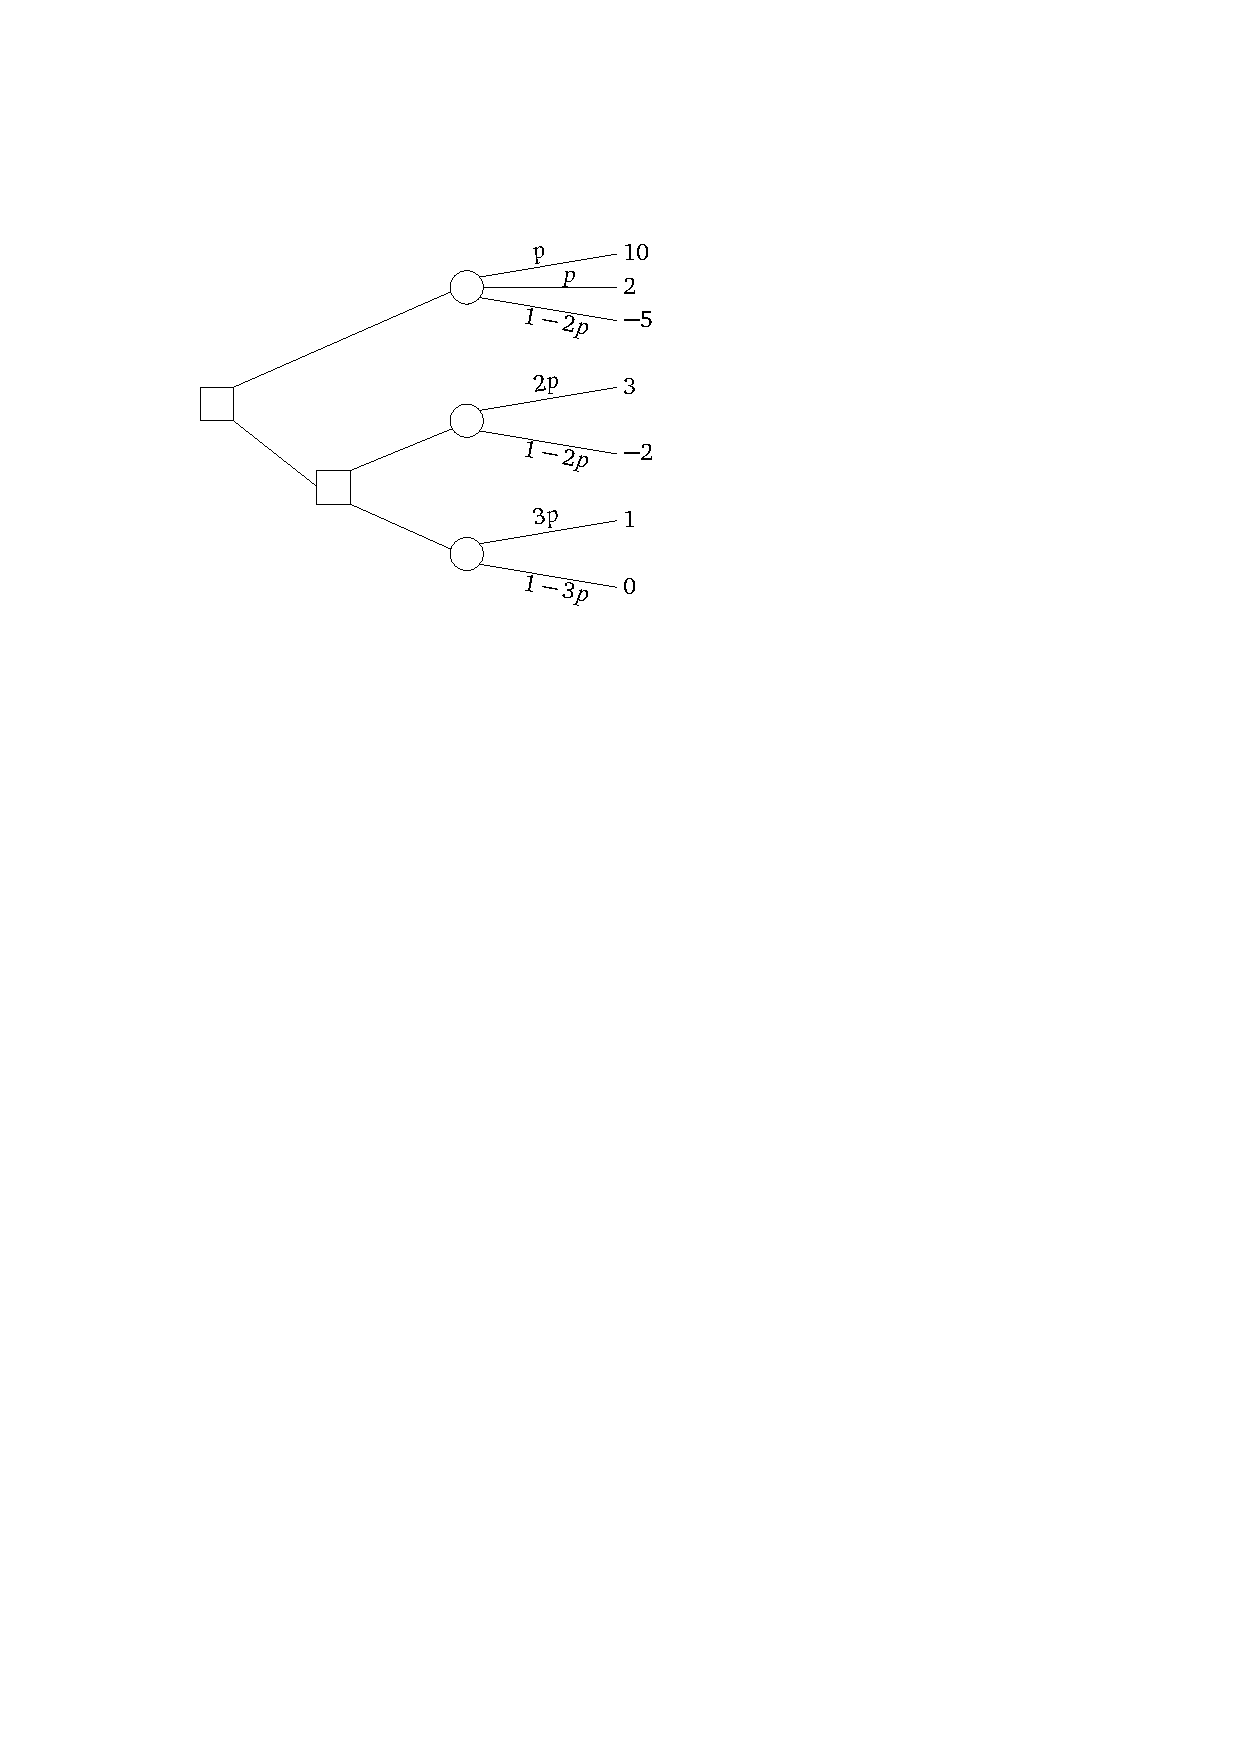
\includegraphics{slike/decision-tree.pdf}
\podnaslov{Odločitveno drevo}
\end{slika}
\end{vprasanje}
\begin{odgovor}
\end{odgovor}
\end{naloga}


\begin{naloga}{Janoš Vidali}{Izpit OR 15.12.2016}
\begin{vprasanje}[avtobus]
Mudi se ti na izpit, a ravno v trenutku,
ko prideš na postajo Konzorcij, odpelje avtobus številka 1.
Na prikazovalniku se izpiše,
da bo naslednji avtobus številka 1 prispel čez $10$ minut,
naslednji avtobus številka 6 čez $6$ minut,
naslednji avtobus številka 14 pa čez $2$ minuti.

Avtobusa 1 in 6 ob ugodnih semaforjih potrebujeta $6$ minut do postaje pri FE,
pri čemer se lahko čas vož\-nje zaradi rdeče luči na semaforju pri FF
podaljša za $1$ minuto.
Verjetnosti, da bo rdečo luč imel avtobus 1, da bo rdečo luč imel avtobus 6,
ter da bosta oba avtobusa imela zeleno luč, so enake $1/3$
(zaradi majhnega razmaka se ne more zgoditi,
da bi oba avtobusa naletela na rdečo luč).
Avtobus številka 1 nadaljuje pot do postaje pri FMF,
za kar potrebuje še $2$ minuti.

Avtobus številka 14 potrebuje $5$ minut do postaje pri študentskih domovih,
od tam pa greš peš do postaje pri FE, za kar potrebuješ še $4$ minute.
Pri tem prečkaš že\-lez\-ni\-co -- če mimo pripelje vlak
(kar se zgodi z verjetnostjo $0.05$),
se čas hoje podaljša za $3$ minute.
Ko prideš na postajo pri FE
(ne glede na to, ali si prišel z avtobusom 6 ali 14),
te čakajo še $4$ minute hoje do FMF,
vendar moraš najprej prečkati Tržaško cesto.
Če je na semaforju rdeča luč
(kar se zgodi z verjetnostjo 0.9, neodvisno od drugih dogodkov),
se lahko odločiš, da $2$ minuti počakaš na zeleno luč in potem nadaljuješ peš,
ali pa da greš nazaj do postaje in počakaš na avtobus številka $1$
(ki bo, tako kot prej, vozil še $2$ minuti do FMF).

Kakšne bodo tvoje odločitve,
da bo pričakovano trajanje poti do FMF čim krajše?
Nariši od\-lo\-čit\-ve\-no drevo
in odločitve sprejmi na podlagi izračunanih verjetnosti!
Glej sliko~\fig{} za shemo možnih poti.

\begin{slika}
\pgfslika
\podnaslov{Shema možnih poti}
\end{slika}
\end{vprasanje}
\begin{odgovor}
\end{odgovor}
\end{naloga}


\begin{naloga}{Janoš Vidali}{Izpit OR 31.1.2017}
\begin{vprasanje}
Dve podjetji bosta predstavili konkurenčna izdelka.
Možnost imaš kupiti delnice prvega podjetja za ceno $10000 €$
ali delnice drugega podjetja po ceni $5000 €$,
lahko pa se seveda odločiš tudi, da delnic ne kupiš.
Ocenjuješ, da bo z verjetnostjo $0.4$ uspelo prvo podjetje,
z verjetnostjo $0.1$ bo uspelo drugo podjetje,
z verjetnostjo $0.5$ pa ne bo uspelo nobeno izmed njiju
(ne more se zgoditi, da bi obe uspeli).
Ob uspehu prvega podjetja se bo vrednost njihovih delnic potrojila,
ob uspehu drugega podjetja pa se bo vrednost njihovih delnic popeterila
-- če si lastiš delnice uspešnega podjetja, jih torej lahko prodaš,
pri čemer bo torej dobiček enak
dvakratniku oziroma štirikratniku vloženega zneska.
Delnic neuspešnega podjetja ne bo želel nihče kupiti,
tako da je v tem primeru vloženi znesek izgubljen.

Za mnenje lahko povprašaš tržnega izvedenca,
ki bo po opravljeni raziskavi povedal,
katero od dveh podjetij ima večje možnosti za uspeh.
Če bo uspešno prvo podjetje, bo to pravilno napovedal z verjetnostjo $0.8$,
če pa bo uspešno drugo podjetje,
bo to pravilno napovedal z verjetnostjo $0.7$.
V primeru, ko podjetji ne bosta uspeli,
bo z verjetnostjo $0.4$ večje možnosti pripisal prvemu,
z verjetnostjo $0.6$ pa drugemu podjetju.
Za svoje mnenje izvedenec računa $1000 €$.

Kakšne bodo tvoje odločitve,
da bo tvoj pričakovani dobiček po odprodaji delnic čim večji?
Nariši od\-lo\-čit\-ve\-no drevo
in odločitve sprejmi na podlagi izračunanih verjetnosti.
Pričakovani dobiček tudi izračunaj.
\end{vprasanje}
\begin{odgovor}
\end{odgovor}
\end{naloga}


\begin{naloga}{Janoš Vidali}{Izpit OR 10.7.2017}
\begin{vprasanje}
Proti računalniškemu programu igraš Texas hold 'em poker.
Pravila igre tukaj niso pomembna.
Ker imaš dostop do kode programa, poznaš logiko, po kateri se ravna.
V trenutni igri si vložil $30$ žetonov, enako tudi nasprotnik.
Nasprotnik z verjetnostjo $0.6$ meni, da so odprte karte ugodnejše zate,
z verjetnostjo $0.4$ pa, da so ugodnejše zanj
(sam si ne ustvariš nobenega mnenja).
V prvem primeru je verjetnost, da so dejansko tvoje karte boljše, enaka $0.8$,
v drugem pa le $0.1$.

Nasprotnik se bo sedaj odločil, ali naj vloži še $10$ žetonov.
Sam se lahko nato odločiš, ali boš vložil $0$, $10$ ali $20$ žetonov
(skupni vložek bo torej $30$, $40$ ali $50$ žetonov).
Če je tvoj vložek manjši od nasprotnikovega,
je igra izgubljena in izgubiš do sedaj vloženo.
Če je tvoj vložek enak na\-sprot\-ni\-ko\-ve\-mu,
z nasprotnikom pogledata karte in tako določita zmagovalca.
Če je tvoj vložek višji od nasprotnikovega,
ima ta možnost odstopiti (tako pridobiš nasprotnikov vložek),
ali pa izenačiti, nakar se zmagovalec določi na podlagi kart.
Če zmagaš, pridobiš nasprotnikov vložek,
če izgubiš, pa izgubiš svojega.

V spodnji tabeli so zbrane verjetnosti dogodkov
v odvisnosti od nasprotnikovega mnenja glede kart.
Verjetnosti navedenih dogodkov pri istem mnenju so med seboj neodvisne.
\begin{center}
\makebox[\textwidth][c]{
\begin{small}
\begin{tabular}{r|cc}
dogodek $\setminus$ nasprotnikovo mnenje
& ugodnejše karte zate & za nasprotnika \\ \hline
dejansko imaš boljše karte & 0.8 & 0.1 \\
nasprotnik vloži $10$ žetonov po razkritju karte & 0.3 & 0.8 \\
nasprotnik izenači skupni vložek $40$ žetonov & 0.2 & 0.7 \\
nasprotnik izenači skupni vložek $50$ žetonov & 0.1 & 0.8
\end{tabular}
\end{small}
}
\end{center}
Na primer:
\begin{multline*}
\Pr[\text{nasprotnik izenači skupni vložek $40$ žetonov} \ | \\
| \ \text{nasprotnikovo mnenje je ``ugodnejše karte zate''}] = 0.2 .
\end{multline*}

Kakšne bodo tvoje odločitve,
da bo tvoj pričakovani dobiček po koncu igre čim večji?
Nariši odločitveno drevo
in odločitve sprejmi na podlagi izračunanih verjetnosti.
Pričakovani dobiček tudi izračunaj.
\end{vprasanje}
\begin{odgovor}
\end{odgovor}
\end{naloga}


\begin{naloga}{Janoš Vidali}{Izpit OR 29.8.2017}
\begin{vprasanje}[dectree2]
Dano je odločitveno drevo s slike~\fig{},
pri čemer velja $0 \le p \le 1/4$.
Pričakovano vred\-nost želimo maksimizirati.
Poišči optimalne odločitve in pričakovano vrednost
v odvisnosti od vrednosti parametra $p$.

\begin{slika}
\pgfslika
\podnaslov{Odločitveno drevo}
\end{slika}
\end{vprasanje}
\begin{odgovor}
\end{odgovor}
\end{naloga}


\begin{naloga}{Janoš Vidali}{Kolokvij OR 23.4.2018}
\begin{vprasanje}
Mladi podjetnik je razvil inovativen izdelek
in se odloča za nadaljnje korake pri njegovem trženju.
Naenkrat lahko naroči izdelavo $500$ izdelkov po ceni $10000 €$
ali $1000$ izdelkov po ceni $18000 €$,
lahko se pa odloči tudi, da izdelave ne naroči.
Podjetnik ocenjuje, da je izdelek tržno zanimiv z verjetnostjo $0.8$.
Odloča se, ali naj posamezen izdelek prodaja po ceni $50 €$ ali $60 €$,
pri čemer so v spodnji tabeli zbrana pričakovana števila prodanih kosov
v odvisnosti od teh pogojev.

\begin{center}
\begin{tabular}{c|cc}
& cena $50 €$ & cena $60 €$ \\
\hline
tržno zanimiv & $650$ & $550$ \\
tržno nezanimiv & $250$ & $100$ \\
\end{tabular}
\end{center}

Predpostavi, da se bodo prodali vsi izdelani kosi,
če je število teh manjše od pričakovane prodaje pri danih pogojih.

\begin{enumerate}[(a)]
\item Kako naj se podjetnik odloči, da bo pričakovani zaslužek čim večji?
Nariši od\-lo\-čit\-ve\-no drevo in ga uporabi pri sprejemanju odločitev.

\item V zadnjem trenutku je podjetnik izvedel,
da bo Podjetniški pospeševalnik objavil
razpis za nagrado za najboljši izdelek.
Razpisni pogoji zahtevajo,
da se za potrebo kontrole kvalitete izdela vsaj $1000$ izdelkov,
od katerih komisija izbere $20$ za dejansko kontrolo,
z ostalimi pa lahko prijavitelj prosto razpolaga.
Če podjetnik zmaga, bo dobil nagrado v višini $k$ evrov,
pri čemer $k \in [1000, 5000]$ še ni znan,
poleg tega pa si obeta tudi $20\%$ povečanje
pričakovanega števila prodanih kosov (v vseh zgoraj omenjenih pogojih).
Če ne zmaga, se pričakovanja ne spremenijo.
Podjetnik ocenjuje, da je verjetnost zmage enaka $0.6$,
če je izdelek tržno zanimiv,
in $0.1$, če izdelek ni tržno zanimiv.

Naj se podjetnik prijavi na razpis?
Nariši odločitveno drevo in odločitve sprejmi v odvisnosti od parametra $k$!
\end{enumerate}
\end{vprasanje}
\begin{odgovor}
\end{odgovor}
\end{naloga}


\begin{naloga}{Janoš Vidali}{Izpit OR 11.6.2018}
\begin{vprasanje}[vrac]
Podajamo se na pot v mesto na drugi strani gorovja.
Lahko se odločimo za pot po cesti okoli gorovja,
za kar bomo porabili $12$ ur.
Vendar pa nas najkrajša pot vodi čez prelaz,
ki je eno uro stran od začetne lokacije.
Žal pa so razmere v gorah nepredvidljive:
ocenjujemo, da bo z verjetnostjo $0.2$ prelaz čist
in ga bomo lahko prevozili v $5$ urah,
z ve\-rjet\-nost\-jo $0.1$ bo delno zasnežen in ga bomo prevozili v $9$ urah,
z verjetnostjo $0.7$ pa bo neprevozen,
zaradi česar se bomo morali vrniti na začetek in iti okoli gorovja
(skupno trajanje poti bo v tem primeru torej $14$ ur).

Edini, ki nam lahko kakorkoli pomaga pri oceni vremenskih razmer na prelazu,
je lokalni vrač,
ki pa živi v dolini pod goro in ne uporablja sodobne tehnologije,
s katero bi ga lahko kontaktirali.
Rade volje pa nam bo povedal, ali na gori vlada mir,
če se na poti do prelaza ustavimo pri njem.
Pogojne verjetnosti njegovega odgovora v odvisnosti od razmer na prelazu
so podane v spodnji tabeli.
\begin{center}
\makebox[\textwidth][c]{
\begin{tabular}{c|ccc}
$P\left(\text{vračev odgovor} \;\middle|\; \text{razmere na prelazu}\right)$
& čist & delno zasnežen & neprevozen \\ \hline
na gori vlada mir & $0.9$ & $0.5$ & $0.1$ \\
na gori divja vojna & $0.1$ & $0.5$ & $0.9$
\end{tabular}
}
\end{center}
Do vrača imamo eno uro vožnje, do prelaza pa potem še eno uro.
Če se po obisku vrača odločimo za pot okoli gorovja,
bomo za nadaljnjo pot porabili $12$ ur.

Kako se bomo odločili?
Nariši odločitveno drevo in ga uporabi pri sprejemanju odločitev.
Izračunaj tudi pričakovano trajanje poti.
Glej sliko~\fig{} za shemo možnih poti.

\begin{slika}
\pgfslika
\podnaslov{Shema možnih poti}
\end{slika}
\end{vprasanje}
\begin{odgovor}
\end{odgovor}
\end{naloga}


\begin{naloga}{Janoš Vidali}{Izpit OR 28.8.2018}
\begin{vprasanje}[dectree3]
Dano je odločitveno drevo s slike~\fig{},
pri čemer velja $0 \le p \le 1$.
Pričakovano vred\-nost želimo maksimizirati.
Poišči optimalne odločitve in pričakovano vrednost
v odvisnosti od vrednosti parametra $p$.

\begin{slika}
\pgfslika
\podnaslov{Odločitveno drevo}
\end{slika}
\end{vprasanje}
\begin{odgovor}
\end{odgovor}
\end{naloga}


\begin{naloga}{?}{Kolokvij OR 26.1.2010}
\begin{vprasanje}[ajkalaj]
V ugledni banki nameravajo okrepiti upravni odbor
z direktorjem za informacijske tehnologije.
Za svetovanje in pridobivanje kandidatov za to mesto
so prosili znano agencijo za kadrovsko svetovanje {\em Kadria d.o.o.}
Ti so jim priporočili prodornega g.~Miho Ajkalaja.
Po intervjuju z g.~Ajkalajem je direktor ocenil,
da bo g.~Ajkalaj z verjetnostjo $p = 3/5$ v enem letu uspešen pri svojem delu.
Če bo uspešen, bo banka dodatno prislužila $2.100.000 €$,
sicer pa bo pridelala dodatno izgubo $800.000 €$
(izobraževanje, vpeljava, odpravnina, \dots).

\begin{enumerate}[(a)]
\item Modeliraj problem v okviru teorije odločanja (stanja, odločitve).
Kakšno odločitev svetuješ direktorju glede na pričakovni dobiček?
Kako je odločitev odvisna od verjetnosti $p$?
Nariši graf, ki prikazuje optimalni pričakovani dobiček v odvisnosti od $p$.

\item Za dodatnih $80.000 €$ lahko agencija
z g.~Ajkalajem opravi dodatne inteligenčne in psihološke teste,
s katerimi lahko ugotovi, ali bo g.~Ajkalaj uspešen.
Statistični povzetek uspešnosti metode v preteklosti je naslednji:
\begin{center}
\begin{tabular}{l|cc}
$P(\text{izid testa} \;|\; \text{posl.~rezultat})$ &
\multicolumn{2}{c}{Izid testa} \\
Poslovni rezultat & pozitiven & negativen \\ \hline
uspešen   &  $7/8$ & $1/8$ \\
neuspešen &  $1/4$ & $3/4$
\end{tabular}
\end{center}
Izračunaj $\EVPI$ in $\EVE$ ter komentiraj,
ali je smiselno izvesti dodatna testiranja.

\item Nariši drevo odločitev in ugotovi,
ali naj direktor izvede testiranje in če ga,
kako naj se odloči glede zaposlitve g.~Ajkalaja.
\end{enumerate}
\end{vprasanje}

\begin{odgovor}
\begin{enumerate}[(a)]
\item Imamo eno odločitev -- ali naj zaposlimo g.~Ajkalaja.
Če ga ne zaposlimo, je dobiček $0 €$,
če pa ga zaposlimo, pa pridemo v stanje,
v katerem imamo z verjetnostjo $p$ dobiček $2.100.000 €$,
z verjetnostjo $1-p$ pa $-800.000 €$.
V tem stanju je torej pričakovan dobiček enak
$$
p \cdot 2.100.000 € - (1-p) \cdot 800.000 € =
p \cdot 2.900.000 € - 800.000 € .
$$
Za $p < 8/29$ torej pričakujemo izgubo in se nam ga ne izplača zaposliti,
sicer pa imamo dobiček in se ga nam tako izplača zaposliti.
Graf pričakovanega dobička je prikazan na sliki~\fig{ajkalaj-graf}.
Pri podani vrednosti $p = 3/5$ se nam torej izplača zaposliti g.~Ajkalaja,
saj tedaj pričakujemo dobiček $940.000 €$.

\item $\EVPI$ izračunamo tako,
da od pričakovanega dobička pri znanem izidu
odštejemo pričakovani dobiček pri neznanem izidu:
$$
\EVPI = 3/5 \cdot 2.100.000 € + 2/5 \cdot 0€ - 940.000 € = 320.000 €
$$
Ker je $\EVPI$ večji od cene dodatnega testiranja,
izračunajmo še $\EVE$.
Najprej določimo verjetnosti:
\begin{align*}
P(\text{test pozitiven}) = 7/8 \cdot 3/5 + 1/4 \cdot 2/5 &= 5/8 \\
P(\text{test negativen}) = 1/8 \cdot 3/5 + 3/4 \cdot 2/5 &= 3/8 \\
P(\text{uspešen rezultat} \;|\; \text{test pozitiven}) =
{7/8 \cdot 3/5 \over 5/8} &= 21/25 \\
P(\text{neuspešen rezultat} \;|\; \text{test pozitiven}) =
{1/4 \cdot 2/5 \over 5/8} &= 4/25 \\
P(\text{uspešen rezultat} \;|\; \text{test negativen}) =
{1/8 \cdot 3/5 \over 3/8} &= 1/5 \\
P(\text{neuspešen rezultat} \;|\; \text{test negativen}) =
{3/4 \cdot 2/5 \over 3/8} &= 4/5
\end{align*}
Sedaj lahko izračunamo $\EVE$:
\begin{multline*}
\EVE = (21/25 \cdot 2.100.000 € - 4/25 \cdot 800.000 €) \cdot 5/8 \, + \\
(1/5 \cdot 0 € + 4/5 \cdot 0 €) \cdot 3/8 - 940.000 € = 82.500 €
\end{multline*}
Ker je $\EVE$ večji od cene testiranja, se torej odločimo za testiranje.

\item Odločitveno drevo je prikazano na sliki~\fig{ajkalaj-drevo}.
Odločimo se za test -- če je ta pozitiven, zaposlimo g.~Ajkalaja, sicer pa ne.
\end{enumerate}

\begin{slika}
\pgfslika[ajkalaj-graf]
\podnaslov[\res{}(a)]{Graf pričakovanega dobička}
\end{slika}

\begin{slika}
\makebox[\textwidth][c]{
\pgfslika[ajkalaj-drevo]
}
\podnaslov[\res{}(c)]{Odločitveno drevo}
\end{slika}
\end{odgovor}
\end{naloga}


\begin{naloga}{?}{Izpit OR 28.6.2010}
\begin{vprasanje}[bp]
Na naftni ploščadi podjetja BP
je prišlo do nekontroliranih izpustov nafte iz vrtine v zalivu.
Po vseh mogočih podvigih, da bi zamašili vrtino,
se je ob\-upa\-no vodstvo podjetja pod pritiski predsednika bližnje države
začelo dobivati z ruskimi strokovnjaki
za mašenje vrtin s pomočjo jedrskih eksplozij pod vodstvom
prof.~dr.~Mikhaila Razturoviča Totalkova.
Vodstvo BP ocenjuje, da bo ekipa dr.~Totalkova
z verjetnostjo $p = 3/7$ uspešno zamašila vrtino.
Tako bo podjetje imelo sicer samo $2.8$ milijarde USD dobička,
sicer pa bi zaradi upada dobička in povzročene škode
utrpeli izgubo $700$ milijonov USD.

\begin{enumerate}[(a)]
\item Modeliraj problem v okviru teorije odločanja (stanja, odločitve).
Kakšno odločitev svetuješ vodstvu BP?
Kako je odločitev odvisna od verjetnosti $p$?
Nariši graf, ki prikazuje optimalni pričakovani dobiček v odvisnosti od $p$.

\item Za dodatnih $90.000$ USD lahko podjetje BP naroči študijo
pri kitajskem ljudskem inštitutu za naftne vrtine iz mesta Lanzhou,
ki ocenjuje uspešnost rizičnih projektov,
in bi ocenilo, ali bo ekipa dr.~Totalkov uspešna.
Statistični povzetek uspešnosti raziskav inštituta v preteklosti je naslednji:
\begin{center}
\begin{tabular}{l|cc}
$P(\text{rez.~raziskave} \;|\; \text{rez.~prov})$ &
\multicolumn{2}{c}{Rezultat raziskave inštituta} \\
Rezultat projekta & pozitiven & negativen \\ \hline
uspešen   &  $7/9$ & $2/9$ \\
neuspešen &  $1/3$ & $2/3$
\end{tabular}
\end{center}
Izračunaj $\EVPI$ in $\EVE$ ter komentiraj,
ali je smiselno izvesti dodatno raz\-iska\-vo.

\item Nariši drevo odločitev in ugotovi,
ali naj podjetje naroči raziskavo in če jo,
kako naj se odloči glede mašenja vrtine.
\end{enumerate}
\end{vprasanje}
\begin{odgovor}
\end{odgovor}
\end{naloga}


\begin{naloga}{?}{Izpit OR 15.9.2010}
\begin{vprasanje}
Letalska družba namerava nabaviti že rabljeno letalo, ki stane $170.000 €$.
Ocenjujejo, da bodo z njim imeli,
če je odlično ohranjeno, $1.000.000 €$ dobička,
če je zadovoljivo ohranjeno, $340.000 €$ dobička,
in če je slabo ohranjeno, le $10.000 €$ dobička.
Verjetnosti, da je letalo odlično, zadovoljivo ali slabo ohranjeno,
so zaporedoma $0.2$, $0.3$ in $0.5$.
\begin{enumerate}[(a)]
\item Modeliraj problem v okviru teorije odločanja (stanja, odločitve).
Kakšno odločitev svetuješ vodstvu družbe?

\item Družba lahko naroči oceno letala pri izvedenski firmi,
ki zahteva za svoje poročilo $10.000 €$.
Vodstvo družbe takole ocenjuje pogojne verjetnosti:
\begin{center}
\begin{tabular}{c|ccc}
$P(\text{rezultat poročila} \;|\;\ \text{kakovost letala})$
& odlično & zadovoljivo & slabo \\ \hline
ugodno & 0.9 & 0.6 & 0.1 \\
neugodno & 0.1 & 0.4 & 0.9
\end{tabular}
\end{center}
Kako naj se vodstvo družbe odloči?
\end{enumerate}

\end{vprasanje}
\begin{odgovor}
\end{odgovor}
\end{naloga}


\begin{naloga}{?}{Kolokvij OR 24.1.2011}
\begin{vprasanje}
Študent tretjega letnika finančne matematike se mora odločiti,
ali bi nadaljeval študij na drugi stopnji.
Ocenjuje, da bo, če študij uspešno zaključi,
v življenju zaslužil $200.000 €$ več,
kot če študij zaključi že po prvi stopnji.
Če pa študija ne zaključi uspešno,
bo imel zaradi stroškov študija in izgubljenega dohodka $40.000 €$ izgube.
Verjetnost, da bo študij na drugi stopnji uspešno zaključil, je $80 \%$.
\begin{enumerate}[(a)]
\item Modeliraj problem v okviru teorije odločanja (stanja, odločitve).
Kakšno odločitev svetuješ študentu?

\item Matematični oddelek ponuja dodatno testiranje,
ki študentom pomaga pri odločitvi, ali naj nadaljujejo študij.
Test stane $500$ evrov,
iz izkušenj kolegov pa študent ocenjuje,
da so pogojne verjetnosti naslednje:
\begin{center}
\begin{tabular}{c|cc}
$P(\text{rezultat testa} \;|\; \text{uspešnost študija})$
& uspešen & neuspešen \\ \hline
pozitiven & $19/20$ & $1/10$ \\
negativen & $1/20$ & $9/10$
\end{tabular}
\end{center}
Ali naj se študent prijavi na dodatno testiranje?
\end{enumerate}
\end{vprasanje}
\begin{odgovor}
\end{odgovor}
\end{naloga}


\begin{naloga}{?}{Izpit OR 9.2.2011}
\begin{vprasanje}
Direktorica banke se mora odločiti, ali bi stranki, računalniškemu podjetju,
odobrila posojilo v vrednosti $100.000 €$.
Po izkušnjah banke so računalniška podjetja neuspešna z verjetnostjo $20 \%$,
povprečno uspešna z verjetnostjo $50 \%$ in uspešna z verjetnostjo $30 \%$.
Če damo podjetju kredit in se izkaže za neuspešno,
bomo imeli v povprečju za $15.000 €$ izgube,
če je povprečno upešno, bomo imeli $10.000 €$ dobička,
če pa je uspešno, bomo imeli $20.000 €$ dobička.
\begin{enumerate}[(a)]
\item Modeliraj problem v okviru teorije odločanja (stanja, odločitve).
Kakšno odločitev svetuješ direktorici banke?
Kolikšen je EVPI?

\item Za ceno $5.000 €$ lahko najamemo podjetje,
ki natančno preuči računalniško podjetje in poda svojo oceno:
negativno, nevtralno ali pozitivno.
Po podatkih banke so pogojne verjetnosti
$P(\text{rezultat testa} \;|\; \text{uspešnost podjetja})$ naslednje:
\begin{center}
\begin{tabular}{c|ccc}
& neuspešno & povprečno uspešno & uspešno \\ \hline
negativno & $1/2$  & $2/5$  & $1/5$ \\
nevtralno & $2/5$  & $1/2$  & $2/5$ \\
pozitivno & $1/10$ & $1/10$ & $2/5$
\end{tabular}
\end{center}
Izračunaj EVE in nariši odločitveno drevo.
Kakšno odločitev svetuješ direktorici banke?
\end{enumerate}
\end{vprasanje}
\begin{odgovor}
\end{odgovor}
\end{naloga}


\begin{naloga}{?}{Vaje OR 11.4.2008}
\begin{vprasanje}
Janez želi naložiti vsoto $1000 €$ v banko za dobo petih let.
Odloča se med tem, da bi jo vezal za pet let (obrestna mera $5\%$)
ali pa petkrat zaporedoma po eno leto (obrestna mera $4\%$).
Če denar veže za pet let, vmes pa varčevanje prekine,
mu pripada le obrestna mera $3\%$.
Ocenjuje, da lahko v naslednjih petih letih pride do naslednjih situacij:
\begin{itemize}
\item varčeval bo pet let, pri tem se obrestna mera ne spremeni,
\item varčeval bo pet let, obrestna mera se po treh letih poveča za $30\%$,
\item varčeval bo pet let, obrestna mera se po treh letih zmanjša za $20\%$,
\item varčeval bo tri leta.
\end{itemize}
Opiši, kako naj se odloči glede na posamezne kriterije
(optimist, pesimist, Laplace, Savage).
Določi vrednosti parametera $\alpha$,
pri katerih je po Hurwiczevem kriteriju možnih več enakovrednih odločitev.
\end{vprasanje}

\begin{odgovor}
Zaradi enostavnosti predpostavimo,
da se obrestuje samo glavnica (enkrat na leto),
pri čemer pri petletnem varčevanju vsakič velja začetna obrestna mera.
Izračunajmo obresti po petih letih pri različnih shemah vezave
glede na dogajanje po treh letih:
\begin{center}
\begin{tabular}{c|cccc}
shema & nespremenjena & povečana & zmanjšana & prekinitev \\ \hline
$5$ let              & $250$ & $250$ & $250$ &   $-$ \\
$3 + 2 \cdot 1$ leto & $170$ & $194$ & $154$ &   $-$ \\
$3$ leta             &  $90$ &  $90$ &  $90$ &  $90$ \\ \hline
$5 \cdot 1$ leto     & $200$ & $224$ & $184$ &   $-$ \\
$3 \cdot 1$ leto     & $120$ & $120$ & $120$ & $120$ \\
\end{tabular}
\end{center}
Drugih možnosti ne bomo obravnavali,
saj se očitno $5$-letna vezava ne izplača, če jo bomo predčasno prekinili.
Iz zgornje tabele je torej jasno,
da se bomo odločili bodisi za $5$-letno vezavo ali pa vsakoletno vezavo,
z morebitno prekinitvijo oziroma prenehanjem po $3$ letih
brez nadaljnje vezave.
Dobimo torej sledečo odločitveno tabelo:
\begin{center}
\begin{tabular}{c|cccc}
začetna shema & nespremenjena & povečana & zmanjšana & prekinitev \\ \hline
$5$ let          & $250$ & $250$ & $250$ &  $90$ \\
$5 \cdot 1$ leto & $200$ & $224$ & $184$ & $120$ \\
\end{tabular}
\end{center}

Pri optimistovem kriteriju se ravnamo glede na najboljši možen izid.
Pri $5$-letni vezavi je to $250 €$, pri letni vezavi pa $224 €$,
zato se odločimo za $5$-letno vezavo.

Pri pesimistovem (Waldovem) kriteriju se ravnamo glede na najslabši možen izid.
Pri $5$-letni vezavi je to $90 €$, pri letni vezavi pa $120 €$,
zato se odločimo za letno vezavo.

Pri Laplaceovem kriteriju so vse možnosti enako verjetne.
Pri $5$-letni vezavi je torej pričakovani dobiček enak
$(250 € + 250 € + 250 € + 90 €)/4 = 210 €$,
pri letni vezavi pa $(200 € + 224 € + 184 € + 120 €)/4 = 182 €$,
zato se odločimo za $5$-letno vezavo.

Pri Savageovem kriteriju želimo minimizirati največje možno obžalovanje.
Pri $5$-letni vezavi je največje obžalovanje enako $120 € - 90 € = 30 €$,
pri letni vezavi pa $250 € - \min\{200€, 224€, 184€\} = 66 €$,
zato se odločimo za $5$-letno vezavo.

Pri Hurwiczevem kriteriju upoštevamo,
da se najboljši izid zgodi z ve\-rjet\-nost\-jo $\alpha$,
najslabši pa z verjetnostjo $1 - \alpha$.
Pri $5$-letni vezavi je torej pričakovan dobiček enak
$\alpha \cdot 250 € + (1 - \alpha) \cdot 90 € = \alpha \cdot 160 € + 90 €$,
pri letni vezavi pa
$\alpha \cdot 224 € + (1 - \alpha) \cdot 120 € = \alpha \cdot 104 € + 120 €$.
Pri vrednosti $\alpha = 15/28$ sta obe možnosti enakovredni.
Pri večjih vrednostih $\alpha$ se odločimo za $5$-letno vezavo,
pri manjših pa za letno vezavo.
\end{odgovor}
\end{naloga}


\begin{naloga}{?}{Kolokvij OR 17.4.2013}
\begin{vprasanje}
Na letalu je $100$ sedežev.
Dane so naslednje verjetnosti za število potnikov,
ki ne pridejo na vkrcanje,
pri čemer je $P(i)$ verjetnost, da natanko $i$ potnikov ne pride na vkrcanje:
$$
P(0) = 0.25, \quad P(1) = 0.5, \quad P(2) = 0.25 .
$$
\begin{enumerate}[(a)]
\item Koliko letalskih kart naj proda letalska družba,
če vsak prazen sedež na letalu prinese $100 €$ izgube,
vsak nezadovoljen potnik, ki ne dobi sedeža, pa $200 €$ izgube?

\item Za $200 €$ lahko izvedemo predhodno analizo,
ki nam napove število potnikov, ki jih ne bo na vkrcanju.
Zanesljivost analize je podana z verjetnostmi
$$
(p_{ij})_{i,j=0}^2 = \begin{bmatrix}
0.7 & 0.1 & 0 \\
0.2 & 0.8 & 0.1 \\
0.1 & 0.1 & 0.9 \\
\end{bmatrix} ,
$$
kjer je $p_{ij}$ verjetnost,
da analiza napove odpoved $i$ potnikov v primeru,
ko imamo dejansko $j$ odpovedi.
Ali naj letalska družba izvede analizo pred prodajo kart?
\end{enumerate}
\end{vprasanje}
\begin{odgovor}
\end{odgovor}
\end{naloga}


\begin{naloga}{?}{Izpit OR 14.6.2013}
\begin{vprasanje}
Fenko, brat škrata Bolfenka, je najboljši alkimist, kar jih je družina imela.
Preživlja se z izdelovanjem zlata iz granodiorita\footnote{
Granodiorit je zelo razširjena magmatska kamnina na Pohorju,
znana tudi kot pohorski tonalit.
}.
Postopek izdelave zlata je naslednji:
ob 23:00 mora nastaviti sveže izkopan granodiorit
($1$ kg svežega granodiorita je vreden $2$ gulda\footnote{
Guld je denarna enota, ki jo uporabljajo pohorski škratje.
})
na točno določeno mesto pod milo nebo\footnote{
Kam je treba nastaviti granodiorit, je odvisno tudi od položaja planetov.
}.
Če nastavljene kamnine noben škrat, srna ali človek ne vidi,
se le-ta v dveh urah spremeni v zlato
(za $1$ kg granodiorita dobi $10$ g zlata).
Verjetnost, da se to zgodi (tj., da nastane zlato), je $2/5$.
To zlato lahko proda škratu zlatarju za gulde
(in to je edini možni način porabe zlata).
Za $10$ g zlata dobi $4$ gulde.
Granodiorit, ki je enkrat že bil nastavljen,
se ne bo nikoli več spremenil v zlato.
Fenko lahko kilogram ``porabljenega'' granodiorita proda za $1$ guld.

Predpostavimo, da Fenko zapravlja denar le za izdelavo zlata iz granodiorita,
da zmeraj nastavi celoštevilsko mnogo kilogramov granodiorita
in ima zmeraj celoštevilsko mnogo guldov
(npr.~s tremi guldi lahko kupi največ $1$ kg granodiorita, en guld mu ostane).

Trenutno ima Fenko $5$ guldov, nič zlata in nič granodiorita.
Koliko kilogramov granodiorita
naj v naslednjih dveh nočeh nastavi pod milo nebo,
da bo imel kar največje pričakovano število guldov?
V odgovoru napiši,
koliko granodiorita naj nastavi prvo noč in koliko drugo noč.
Odgovor bo odvisen od tega,
ali se mu ponoči granodiorit spremeni v zlato ali ne.
\end{vprasanje}
\begin{odgovor}
\end{odgovor}
\end{naloga}


\begin{naloga}{Batagelj, Kaufman}{\cite[Naloga~4.3]{bk}}
\begin{vprasanje}
Ljubo prodaja časopise po centru Ljubljane.
Vsak dan se mora odločiti, koliko časopisov naj naroči.
Za vsak naročen časopis plača $0.8 €$, iztrži pa $1 €$.
Za neprodane časopise ne dobi povrnjenega denarja.
Vsak dan je verjetnost, da bo imel $i$ kupcev, enaka $p_i$,
kjer je $p_6 = 0.1$, $p_7 = 0.2$, $p_8 = 0.3$, $p_9 = 0.3$ in $p_{10} = 0.1$.
\begin{enumerate}[(a)]
\item Kakšno odločitev svetuješ Ljubu in zakaj?
\item Kolikšen zaslužek lahko pričakuje v mesecu,
ko časopis izide petindvajsetkrat?
\end{enumerate}
\end{vprasanje}
\begin{odgovor}
\end{odgovor}
\end{naloga}


\begin{naloga}{?}{Izpit OR 24.6.2014}
\begin{vprasanje}
Tovarna od dobavitelja dobi paket $10$ komponent $A$.
Tovarna sestavlja izdelke $B$,
kjer gre v vsak izdelek $B$ natanko ena komponenta $A$.
Dane so verjetnosti
$$
p_i = P(\text{med $10$ komponentami $A$ je natanko $i$ pokvarjenih}),
$$
kjer je $p_1 = 0.7$, $p_2 = 0.2$ in $p_3 = 0.1$.
Stroški pregleda posamezne komponente so $45 €$.
Stroški popravila izdelka $B$ zaradi vgrajene okvarjene komponente $A$
so enaki $350 €$.
\begin{enumerate}[(a)]
\item Denimo, da ima tovarna na izbiro samo dve možnosti.
Prva je, da pregleda vseh $10$ dobavljenih izdelkov.
Druga možnost pa je, da ne pregleda nobenega dobavljenega izdelka.
Katera odločitev tovarni povzroči manj stroškov?

\item Naj ima sedaj tovarna na voljo drugačni izbiri.
Prva je, da naključno izbere eno izmed $10$ komponent $A$,
jo pregleda in po potrebi zamenja,
ter gre nato direktno v proizvajanje izdelkov $B$.
Druga možnost pa je, da pregleda vseh $10$ izdelkov.
Katera odločitev tovarni povzroči manj stroškov?
\end{enumerate}
\end{vprasanje}
\begin{odgovor}
\end{odgovor}
\end{naloga}


\begin{naloga}{?}{Izpit OR 25.8.2014}
\begin{vprasanje}
V škatli so štirje ponarejeni kovanci, vredni $0 €$,
in en zlat kovanec, vreden $100 €$.
Na slepo lahko izbereš po en kovanec,
pri čemer moraš za vsako izbiranje plačati $30 €$.
Določi povprečen profit, ki ga dosežeš pri igranju te igre.
\end{vprasanje}
\begin{odgovor}
\end{odgovor}
\end{naloga}


\begin{naloga}{?}{Izpit OR 12.5.2016}
\begin{vprasanje}
Smo v letu 2500 in turistične rakete že potujejo na Luno.
LunaAirways oglašuje let, na katerem je lahko $100$ potnikov.
LunaAirways računa, da bodo vsa mesta zasedena.
Z leti izkušenj vedo,
da nekatere potnike zagrabi strah in tako ne pridejo na potovanje.
Ocenjujejo, da je verjetnost $p_i$,
da natanko $i$ potnikov ($0 \le i \le 5$) ne pride na potovanje,
naslednje:
\begin{center}
\begin{tabular}{c|cc}
$i$ & od $0$ do $3$ & od $4$ do $5$ \\ \hline
$p_i$ & $0.2$ & $0.1$
\end{tabular}
\end{center}

S prodajo karte ima družba $300$ denot dobička.
Za vsakega potnika, ki bo moral menjati let,
ima LunaAirways $400$ denot stroškov.
Koliko kart naj proda LunaAirways, če želi maksimizirati pričakovani dobiček?
\end{vprasanje}
\begin{odgovor}
\end{odgovor}
\end{naloga}


\begin{naloga}{?}{Izpit OR 24.5.2016}
\begin{vprasanje}
Kavarna {\em ma$\phi$ja} je razvila recept za novo torto.
Slaščičarna {\em sladkeoperacijskeraziskave}
je za eksluzivno pravico do recepta pripravljena plačati $15002 €$.
Če se kavarna {\em ma$\phi$ja} odloči za samostojno prodajo torte,
jih začetni vložek stane $10000 €$,
za vsako prodano torto pa zaslužijo $25 €$.
Po njihovi presoji
je verjetnost uspeha recepture (prodajo $100000$ tort) enaka $0.4$,
verjetnost propada (prodali bi zgolj $10000$ tort) pa $0.6$.
Kavarna se lahko odloči, da zaprosi za pomoč tudi pod\-jet\-je,
ki na osnovi degustacij torte sestavi mnenje o uspehu recepta.
Svetovanje jih stane $35000 €$,
natančnost svetovanja pa opisuje spodnja tabela.
\begin{center}
\begin{tabular}{c|cc}
$P(\text{mnenje svetovalca} \;|\;\ \text{uspeh recepta})$
& Recept uspe & Recept ne uspe \\ \hline
Ugodno   & ${3 \over 4}$ & ${1 \over 2}$ \\
Neugodno & ${1 \over 4}$ & ${1 \over 2}$
\end{tabular}
\end{center}
Kako naj se kavarna {\em ma$\phi$ja} odloči?
Zakaj?
\end{vprasanje}
\begin{odgovor}
\end{odgovor}
\end{naloga}


\begin{naloga}{?}{Izpit OR 24.5.2016}
\begin{vprasanje}
Organizatorji olimpijskih iger so zgradili dvorano za judo,
ki sprejme $1000$ ljudi.
Popularnost juda je na vrhuncu,
zato organizatorji pričakujejo, da bodo vse karte zakupljene.
Zaradi straha pred virusom zika so analitiki
za $0 \le i \le 5$ ($i \in \Z$) izračunali verjetnosti $p_i$,
da se natanko $i$ izmed imetnikov kart ne pojavi na prireditvi.
Verjetnosti so zbrane v spodnji tabeli.
\begin{center}
\begin{tabular}{c|cccccc}
$i$   & $0$    & $1$    & $2$   & $3$   & $4$    & $5$ \\ \hline
$p_i$ & $0.01$ & $0.19$ & $0.3$ & $0.4$ & $0.05$ & $0.05$
\end{tabular}
\end{center}

S prodajo vstopnice imajo organizatorji $1000$ denot dobička.
Za vsakega obiskovalca,
ki bo ostal brez sedeža in bo moral v VIP sekcijo dvorane,
imajo $1400$ denot stroškov.
Koliko kart naj organizatorji olimpijskih iger prodajo,
če želijo maksimizirati pričakovani dobiček?
\end{vprasanje}
\begin{odgovor}
\end{odgovor}
\end{naloga}

\subsection{Dinamično programiranje}

\begin{naloga}{?}{Vaje OR 6.4.2016}
\begin{vprasanje}
Na avtocestni odsek dolžine $M$ kilometrov
želimo postaviti oglasne plakate.
Dovoljene lokacije plakatov določa urad za oglaševanje
in so predstavljene s števili $x_1, x_2, \dots x_n$,
kjer $x_i$ ($1 \le i \le n$)
predstavlja oddaljenost od začetka odseka v kilometrih.
Profitabilnost oglasa na lokaciji $x_i$ določa vrednost $v_i$
($1 \le i \le n$).
Urad za oglaševanje podaja tudi omejitev,
da mora biti razdalja med oglasi vsaj $d$ kilometrov.
Oglase želimo postaviti tako, da bodo čim bolj profitabilni.
\begin{enumerate}[(a)]
\item Reši problem za parametre $M = 20$, $d = 5$, $n = 8$,
$(x_i)_{i=1}^n = (1, 2, 8, 10, 12,$ $14, 17, 20)$ in
$(v_i)_{i=1}^n = (8, 8, 12, 10, 7, 5, 6, 10)$.
\item Napiši rekurzivne enačbe za opisani problem.
\item Napiši algoritem,
ki poišče najbolj profitabilno postavitev oglasov za dane parametre.
Kakšna je njegova časovna zahtevnost?
\end{enumerate}

\end{vprasanje}
\begin{odgovor}
\end{odgovor}
\end{naloga}


\begin{naloga}{?}{Vaje OR 6.4.2016}
\begin{vprasanje}
Imamo nahrbtnik nosilnosti $M$ kilogramov.
Danih je $n$ objektov z vrednostmi $v_i$ in težami $t_i$ ($1 \le i \le n$).
Problem nahrbtnika sprašuje po izbiri predmetov
$I \subseteq \{1, 2, \dots, n\}$,
ki maksimizira njihovo skupno vrednost pri omejitvi $\sum_{i \in I} t_i \le M$.
\begin{enumerate}[(a)]
\item Napiši rekurzivne enačbe za opisani problem.
\item Z uporabo rekurzivnih enačb reši problem za parametre $M = 8$, $n = 8$,
$(v_i)_{i=1}^n = (9, 9, 8, 11, 10, 15,$ $3, 12)$ in
$(t_i)_{i=1}^n = (3, 5, 1, 4, 3, 8, 2, 7)$.
\end{enumerate}

\end{vprasanje}
\begin{odgovor}
\end{odgovor}
\end{naloga}


\begin{naloga}{?}{Vaje OR 6.4.2016}
\begin{vprasanje}
Dana je matrika $A = (a_{ij})_{i,j=1}^{m,n}$.
Poiskati želimo pot minimalne vsote,
ki se začne v levem zgornjem kotu (pri $a_{11}$)
in konča v desnem spodnjem kotu (pri $a_{mn}$).
Dovoljeni so zgolj premiki v desno in navzdol.
\begin{enumerate}[(a)]
\item Reši problem za matriko
$$
A = \begin{pmatrix}
131 & 673 & 234 & 103 &  18 \\
201 &  96 & 342 & 965 & 150 \\
630 & 803 & 746 & 422 & 111 \\
537 & 699 & 497 & 121 & 956 \\
805 & 732 & 524 &  37 & 332
\end{pmatrix} .
$$
\item Napiši rekurzivne enačbe za opisani problem.
\item Na osnovi rekurzivnih enačb napiši algoritem, ki reši opisani problem.
Oceni tudi njegovo časovno zahtevnost v odvisnosti od $m$ in $n$.
\end{enumerate}

\end{vprasanje}
\begin{odgovor}
\end{odgovor}
\end{naloga}


\begin{naloga}{?}{Vaje OR 6.4.2016}
\begin{vprasanje}
Dan je niz $S = a_1 a_2 \dots a_n$,
kjer so $a_i$ ($1 \le i \le n$) elementi neke končne abecede.
Nizu $a_j a_{j+1} \dots a_k$, kjer je $1 \le j \le k \le n$,
pravimo {\em strnjen podniz} niza $S$.
S pomočjo dinamičnega programiranja napiši algoritem,
ki določi najdaljši palindromski strnjen podniz v $S$.

\end{vprasanje}
\begin{odgovor}
\end{odgovor}
\end{naloga}


\begin{naloga}{?}{Vaje OR 6.4.2016}
\begin{vprasanje}
Dana je matrika $A = (a_{ij})_{i,j=1}^{m,n}$.
Poiskati želimo strnjeno podmatriko matrike $A$
z največjo vsoto komponent.
\begin{enumerate}[(a)]
\item Reši problem za matriko
$$
A = \begin{pmatrix}
 1 & -1 &  2 &  4 \\
-3 & -2 &  8 &  2 \\
-3 &  2 & -2 &  4 \\
 1 & -5 & -1 & -2
\end{pmatrix} .
$$
\item Napiši rekurzivne enačbe za opisani problem.
\item Napiši algoritem, ki reši opisani problem.
Oceni tudi njegovo časovno zahtevnost v odvisnosti od $m$ in $n$.
\end{enumerate}

\end{vprasanje}
\begin{odgovor}
\end{odgovor}
\end{naloga}


\begin{naloga}{?}{Vaje OR 6.4.2016}
\begin{vprasanje}
Na voljo imamo kovance z vrednostmi $1 = v_1 < v_2 < \cdots < v_n$
in vsoto $C$, ki jo želimo izplačati s kovanci.
Predpostavljamo, da imamo dovolj velik nabor kovancev.
\begin{enumerate}[(a)]
\item Poišči izplačilo z najmanjšim številom kovancev
za $C = 25$, $n = 4$ in $(v_i)_{i=1}^n = (1, 2, 5, 7)$.
\item S pomočjo dinamičnega programiranja reši problem v splošnem.
\end{enumerate}

\end{vprasanje}
\begin{odgovor}
\end{odgovor}
\end{naloga}


\begin{naloga}{?}{Vaje OR 6.4.2016}
\begin{vprasanje}
Na ulici je $n$ vrstnih hiš,
pri čemer je v $i$-ti hiši $c_i$ denarja.
Tat se odloča, katere izmed hiš naj oropa.
Vsak oropan stanovalec to sporoči svojim sosedom,
zato tat ne sme oropati dveh sosednjih hiš.
Ker je tat poslušal predmet Operacijske raziskave,
pozna dinamično programiranje.
Pokaži, kako naj tat določi, katere hiše naj oropa.

\end{vprasanje}
\begin{odgovor}
\end{odgovor}
\end{naloga}


\begin{naloga}{?}{Kolokvij OR 31.5.2012}
\begin{vprasanje}
Imamo hlod dolžine $\ell$,
ki bi ga radi razžagali na $n$ označenih mestih
$0 < x_1 < x_2 < \dots < x_n < \ell$.
Eno rezanje stane toliko, kolikor je dolžina hloda, ki ga režemo.
Ko hlod prerežemo, dobimo dva manjša hloda, ki ju režemo naprej.
Poiskati želimo zaporedje rezanj z najmanjšo ceno.
\begin{enumerate}[(a)]
\item Reši problem pri podatkih $\ell = 10$ in $(x)_{i=1}^4 = (3, 5, 7, 8)$.
\item S pomočjo dinamičnega programiranja reši problem v splošnem.
Oceni tudi njegovo časovno zahtevnost.
\end{enumerate}

\end{vprasanje}
\begin{odgovor}
\end{odgovor}
\end{naloga}


\begin{naloga}{Hillier, Lieberman}{\cite[Problem~11.3-1]{hl}}
\begin{vprasanje}
Lastnik verige $n$ trgovin z živili je kupil $m$ zabojev svežih jagod.
Naj bo $p_{ij}$ pričakovan dobiček v trgovini $j$,
če tja dostavimo $i$ zabojev.
Zanima nas, koliko zabojev naj gre v vsako trgovino,
da bomo imeli čim večji zaslužek.
Zaradi logističnih razlogov zabojev ne želimo deliti.
\begin{enumerate}[(a)]
\item Z dinamičnim programiranjem reši problem za podatke $m = 5$, $n = 3$
in $p_{ij}$ iz sledeče tabele:
$$
\begin{array}{c|ccc}
p_{ij} & 1 & 2 & 3 \\
\hline
0 &  0 &  0 &  0 \\
1 &  5 &  6 &  4 \\
2 &  9 & 11 &  9 \\
3 & 14 & 15 & 13 \\
4 & 17 & 19 & 18 \\
5 & 21 & 22 & 20 \\
\end{array}
$$
\item Napiši algoritem, ki reši opisani problem v splošnem.
\end{enumerate}

\end{vprasanje}
\begin{odgovor}
\end{odgovor}
\end{naloga}


\begin{naloga}{Hillier, Lieberman}{\cite[Problem~11.3-8]{hl}}
\begin{vprasanje}
Podjetje bo kmalu uvedlo nov izdelek na zelo konkurenčen trg,
zato trenutno pripravlja marketinško strategijo.
Odločili so se, da bodo izdelek uvedli v treh fazah.
V prvi fazi bodo pripravili posebno začetno ponudbo z močno znižano ceno,
da bi privabili zgodnje kupce.
Druga faza bo vključevala intenzivno oglaševalsko kampanjo,
da bi zgodnje kupce prepričali, naj izdelek še vedno kupujejo po redni ceni.
Znano je, da bo ob koncu druge faze
konkurenčno podjetje predstavilo svoj izdelek.
Zato bo v tretji fazi okrepljeno oglaševanje z namenom,
da bi preprečili beg strank h konkurenci.

Podjetje ima za oglaševanje na voljo $4$ milijone evrov,
ki jih želimo čim bolj učinkovito porabiti.
Naj bo $m$ tržni delež v procentih, pridobljen v prvi fazi,
$f_2$ delež, ohranjen po drugi fazi,
in $f_3$ delež, ohranjen po tretji fazi.
Maksimizirati želimo končni tržni delež, torej količino $m f_2 f_3$.

\begin{enumerate}[(a)]
\item Denimo, da želimo v vsaki fazi porabiti nek večkratnik milijona evrov,
pri čemer bomo pri prvi fazi porabili vsaj milijon evrov.
V spodnji tabeli so zbrani vplivi porabljenih količin
na vrednosti $m$, $f_2$ in $f_3$.
$$
\begin{array}{c|ccc}
M€ & m & f_2 & f_3 \\
\hline
0 &  - & 0.2 & 0.3 \\
1 & 20 & 0.4 & 0.5 \\
2 & 30 & 0.5 & 0.6 \\
3 & 40 & 0.6 & 0.7 \\
4 & 50 &   - &   - \\
\end{array}
$$
Kako naj razdelimo sredstva?
\item Denimo sedaj,
da lahko v vsaki fazi porabimo poljubno pozitivno količino denarja
(seveda glede na omejitev skupne porabe).
Naj bodo torej $x_1$, $x_2$ in $x_3$ količine denarja v milijonih evrov,
ki jih porabimo v prvi, drugi in tretji fazi.
Vpliv na tržni delež je podan s formulami
$$
m = x_1 (10 - x_1), \quad
f_2 = 0.4 + 0.1 x_2, \quad \text{in} \quad
f_3 = 0.6 + 0.07 x_3 .
$$
Kako naj sedaj razdelimo sredstva?
\end{enumerate}

\end{vprasanje}
\begin{odgovor}
\end{odgovor}
\end{naloga}


\begin{naloga}{?}{Izpit OR 26.6.2012}
\begin{vprasanje}
Nori profesor Boltežar stanuje v stolpnici z $n$ nadstropji,
oštevilčenimi od $1$ do $n$.
Nori stanovalci tega bloka radi mečejo cvetlične lončke z balkonov.
Boltežar bi rad ugotovil, katero je najvišje nadstropje,
s katerega lahko pade cvetlični lonček, ne da bi se razbil.
Jasno je, da če se lonček razbije pri padcu iz $k$-tega nadstropja,
potem se razbije tudi pri padcu s $(k+1)$-tega nadstropja.
Če bi Boltežar imel le en cvetlični lonček,
bi ga lahko metal po vrsti od najnižjega nadstropja navzgor,
dokler se ne bi razbil.
V najslabšem primeru bi lonček torej vrgel $n$ krat
(možno je, da bi lonček preživel tudi padec iz najvišjega nadstropja).

Ker ima Boltežar doma $k$ cvetličnih lončkov,
lahko do rezultata pride tudi z manjšim številom metov.
S pomočjo dinamičnega programiranja bi rad poiskal strategijo metanja,
ki bi minimizirala število potrebnih metov v najslabšem primeru.
\begin{enumerate}[(a)]
\item Napiši rekurzivne enačbe za opisani problem.
\item Napiši algoritem, ki reši opisani problem.
Oceni tudi njegovo časovno zahtevnost v odvisnosti od $n$ in $k$.
\end{enumerate}

\end{vprasanje}
\begin{odgovor}
\end{odgovor}
\end{naloga}


\begin{naloga}{Hillier, Lieberman}{\cite[Problem~11.2-2]{hl}}
\begin{vprasanje}
Vodja prodaje pri založniku učbenikov za fakulteto
ima na voljo $6$ trgovskih potnikov,
ki jim želi dodeliti eno od treh regij, v kateri bodo delovali.
V vsaki regiji mora delovati vsaj en trgovski potnik.
Naj bo $p_{ij}$ pričakovana porast v prodaji v regiji $j$,
če bo tam delovalo $i$ trgovskih potnikov:
$$
\begin{array}{c|ccc}
p_{ij} & 1 & 2 & 3 \\
\hline
1 & 35 & 21 & 28 \\
2 & 48 & 42 & 41 \\
3 & 70 & 56 & 63 \\
4 & 89 & 70 & 75 \\
\end{array}
$$
Reši problem s pomočjo dinamičnega programiranja.

\end{vprasanje}
\begin{odgovor}
\end{odgovor}
\end{naloga}


\begin{naloga}{Hillier, Lieberman}{\cite[Problem~11.3-16]{hl}}
\begin{vprasanje}
Dan je sledeči nelinearni program.
\begin{align*}
\max &\quad 2x_1^2 + 2x_2 + 4x_3 - x_3^2 \\[1ex]
2x_1 + x_2 + x_3 &\le 4 \\
x_1, x_2, x_3 &\ge 0
\end{align*}
Reši ga s pomočjo dinamičnega programiranja.

\end{vprasanje}
\begin{odgovor}
\end{odgovor}
\end{naloga}


\begin{naloga}{Hillier, Lieberman}{\cite[Problem~11.4-1]{hl}}
\begin{vprasanje}
Igralec na srečo bo odigral tri partije s svojimi prijatelji,
pri čemer lahko vsakič stavi na svojo zmago.
Stavi lahko katerokoli vsoto denarja, ki jo ima na voljo
-- če izgubi partijo, zastavljeno vsoto izgubi, sicer pa tako vsoto pridobi.
Pri vsaki partiji sta verjetnosti zmage in poraza enaki $1/2$.
Na začetku ima $75 €$, na koncu pa želi imeti $100 €$
(ker igra s prijatelji, noče imeti več kot toliko).

Z dinamičnim programiranjem poišči strategijo stavljenja,
ki maksimizira verjetnost, da bo na koncu imel natanko $100 €$.
\end{vprasanje}
\begin{odgovor}
\end{odgovor}
\end{naloga}


\begin{naloga}%
{Dasgupta, Papadimitriou, Vazirani}{\cite[Exercise~6.14]{dpv}}
\begin{vprasanje}[nal:blago]
Imamo pravokoten kos blaga dimenzij $m \times n$,
kjer sta $m$ in $n$ pozitivni celi števili,
ter seznam $k$ izdelkov,
pri čemer potrebujemo za izdelek $i$
pravokoten kos blaga dimenzij $a_i \times b_i$
($a_i, b_i$ sta pozitivni celi števili),
ki ga prodamo za ceno $c_i > 0$.
Imamo stroj, ki lahko poljuben kos blaga razreže na dva dela
bodisi vodoravno, bodisi navpično.
Začetni kos blaga želimo razrezati tako,
da bomo lahko naredili izdelke,
ki nam bodo prinašali čim večji dobiček.
Pri tem smemo izdelati poljubno število kosov posameznega izdelka.
Kose blaga lahko seveda tudi obračamo
(tj., za izdelek $i$ lahko narežemo kos velikosti
$a_i \times b_i$ ali $b_i \times a_i$).

Zapiši rekurzivne enačbe za reševanje danega problema.
Razloži, kaj predstavljajo spremenljivke,
v kakšnem vrstnem redu jih računamo,
ter kako dobimo optimalno rešitev.
\end{vprasanje}
\begin{odgovor}
\end{odgovor}
\end{naloga}


\begin{naloga}{Janoš Vidali}{Izpit OR 15.12.2016}
\begin{vprasanje}
Oceni časovno zahtevnost algoritma,
ki sledi iz rekurzivnih enačb za nalogo~\ref{nal:blago}.
Reši problem za podatke $m = 5, n = 3, k = 4$,
$(a_i)_{i=1}^k = (2, 3, 1, 2)$, $(b_i)_{i=1}^k = (2, 1, 4, 3)$
in $(c_i)_{i=1}^k = (6, 3, 5, 7)$.
\end{vprasanje}
\begin{odgovor}
\end{odgovor}
\end{naloga}


\begin{naloga}{Janoš Vidali}{Izpit OR 31.1.2017}
\begin{vprasanje}
Dano je zaporedje $n$ realnih števil $a_1, a_2, \dots, a_n$.
Želimo poiskati strnjeno podzaporedje z največjim produktom
-- t.j., taka indeksa $i, j$ ($1 \le i \le j \le n$),
da je produkt $a_i a_{i+1} \cdots a_{j-1} a_j$ čim večji.

\begin{enumerate}[(a)]
\item Zapiši rekurzivne enačbe za reševanje danega problema.
Razloži, kaj predstavljajo spremenljivke,
v kakšnem vrstnem redu jih računamo,
ter kako dobimo optimalno rešitev. \\
{\small {\bf Namig:}
posebej obravnavaj pozitivne in negativne delne produkte.}

\item Oceni časovno zahtevnost algoritma, ki sledi iz zgoraj zapisanih enačb.

\item S svojim algoritmom reši problem za zaporedje
$$
0.9, \ -2, \ -0.6, \ -0.5, \ -2, \ 5, \ 0.1, \ 3, \ 0.5, \ -3 \ .
$$
\end{enumerate}
\end{vprasanje}
\begin{odgovor}
\end{odgovor}
\end{naloga}


\begin{naloga}{Sergio Cabello}{Izpit OR 15.3.2017}
\begin{vprasanje}
Za zaporedje števil $x_1, x_2, \dots x_m$ pravimo, da je {\em oscilirajoče},
če velja $x_i < x_{i+1}$ za vse sode $i$ in $x_i > x_{i+1}$ za vse lihe $i$.
S pomočjo dinamičnega programiranja zasnuj algoritem,
ki v polinomskem času izračuna dolžino najdaljšega oscilirajočega podzaporedja
zaporedja celih števil $a_1, a_2, \dots a_n$.
\end{vprasanje}
\begin{odgovor}
\end{odgovor}
\end{naloga}


\begin{naloga}{Janoš Vidali}{Izpit OR 10.7.2017}
\begin{vprasanje}
V podjetju imajo na voljo $m$ milijonov evrov sredstev,
ki jih bodo vložili v razvoj nove aplikacije.
Denar bodo porazdelili med tri skupine.
Naj bodo $x_1$, $x_2$ in $x_3$ količine denarja (v milijonih evrov),
ki jih bodo dodelili razvijalcem, oblikovalcem in marketingu.
Vrednosti $x_1, x_2, x_3$ niso nujno cela števila.
Razvijalci morajo dobiti vsaj $a_1$ milijonov evrov,
potencial, ki ga ustvarijo, pa je $p_1 = n_1 + k_1 x_1$.
Oblikovalci morajo dobiti vsaj $a_2$ milijonov evrov,
potencial, ki ga ustvarijo, pa je $p_2 = n_2 + k_2 x_2$.
Marketing mora dobiti vsaj $a_3$ milijonov evrov,
ustvari pa faktor $p_3 = n_3 + k_3 x_3$.
Pričakovani dobiček v milijonih evrov
se izračuna po formuli $d = (p_1 + p_2) p_3$.
V podjetju bi radi sredstva porazdelili med skupine tako,
da bo pričakovani dobiček čim večji.

\begin{enumerate}[(a)]
\item Zapiši rekurzivne enačbe za reševanje danega problema.
\item Z zgoraj zapisanimi enačbami reši problem
pri podatkih $m = 15$, $a_1 = 4$, $n_1 = 3$, $k_1 = 1.5$,
$a_2 = 3$, $n_2 = 4$, $k_2 = 2$, $a_3 = 2$, $n_3 = 0.4$ in $k_3 = 0.3$.
\end{enumerate}
\end{vprasanje}
\begin{odgovor}
\end{odgovor}
\end{naloga}


\begin{naloga}{Janoš Vidali}{Izpit OR 29.8.2017}
\begin{vprasanje}
V veliki multinacionalni korporaciji želijo,
da bi se zakonodaja spremenila v njihov prid.
V ta namen so najeli $m$ lobistov,
ki se bodo pogajali z $n$ političnimi strankami,
da pridobijo njihovo podporo pri spremembi zakonodaje.
Vsak lobist se bo pogajal s samo eno stranko;
k vsaki stranki lahko pošljejo več lobistov.
Naj bo $p_{ij}$ ($0 \le i \le m$, $1 \le j \le n$) verjetnost,
da pridobijo podporo stranke $j$,
če se z njo pogaja $i$ lobistov
(lahko predpostaviš $p_{i-1,j} \le p_{ij}$ za vsaka $i, j$).
Verjetnosti za različne stranke so med seboj neodvisne.
Maksimizirati želijo verjetnost,
da bodo lobisti pridobili podporo vseh $n$ političnih strank.

\begin{enumerate}[(a)]
\item Zapiši rekurzivne enačbe za reševanje danega problema.
\item Naj bo $m = 6$ in $n = 3$.
K vsaki stranki želijo poslati vsaj enega lobista
(tj., $p_{0j} = 0$ za vsak $j$),
vrednosti $p_{ij}$ za $i \ge 1$ pa so podane v spodnji tabeli.
$$
\begin{array}{c|ccc}
p_{ij} & 1 & 2 & 3 \\ \hline
1 & 0.2 & 0.4 & 0.3 \\
2 & 0.5 & 0.5 & 0.4 \\
3 & 0.7 & 0.5 & 0.8 \\
4 & 0.8 & 0.6 & 0.9 \\
\end{array}
$$
Za dane podatke reši problem z zgoraj zapisanimi enačbami.
\end{enumerate}
\end{vprasanje}
\begin{odgovor}
\end{odgovor}
\end{naloga}


\begin{naloga}{Janoš Vidali}{Kolokvij OR 23.4.2018}
\begin{vprasanje}[nal:domine]
Imamo zaporedje $n$ polj,
pri čemer je na $i$-tem polju zapisano število $a_i$.
Na voljo imamo še $\lfloor n/2 \rfloor$ domin,
z vsako od katerih lahko pokrijemo dve sosednji polji.
Vsaka domina je sestavljena iz dveh delov:
na enem je znak $+$, na drugem pa znak $-$.
Posamezno polje lahko pokrijemo z le eno domino;
če sta pokriti dve sosednji polji, morata biti pokriti z različnima znakoma
(bodisi z iste, bodisi z druge domine).
Iščemo tako postavitev domin,
ki maksimizira vsoto pokritih števil,
pomnoženih z znakom na delu domine, ki pokriva število.
Pri tem ni potrebno, da uporabimo vse domine.
Primer je podan na sliki~\ref{fig:domine}.

\begin{enumerate}[(a)]
\item Zapiši rekurzivne enačbe za reševanje danega problema.
Razloži, kaj predstavljajo spremenljivke,
v kakšnem vrstnem redu jih računamo,
ter kako dobimo optimalno rešitev. \\
{\small {\bf Namig:}
posebej obravnavaj dva primera glede na postavitev zadnje domine.}

\item Oceni časovno zahtevnost algoritma, ki sledi iz zgoraj zapisanih enačb.

\item S svojim algoritmom poišči optimalno pokritje
za primer s slike~\ref{fig:domine}.
\end{enumerate}

\begin{figure}
\centering
\begin{tikzpicture}[style=thick,scale=1.2]
\tikzstyle{field}=[rectangle, minimum size=10mm]
\tikzstyle{domino}=[field, draw, minimum size=8mm]

\node[field] at (0, 0) {$6$};
\node[field] at (1, 0) {$3$};
\node[field] at (2, 0) {$-4$};
\node[field] at (3, 0) {$2$};
\node[field] at (4, 0) {$-3$};
\node[field] at (5, 0) {$5$};
\node[field] at (6, 0) {$9$};
\node[field] at (7, 0) {$1$};
\node[field] at (8, 0) {$2$};

\node[domino] at (1.1, 1) {$\pp$};
\node[domino] at (1.9, 1) {$\mm$};
\node[domino] at (5.1, 1) {$\mm$};
\node[domino] at (5.9, 1) {$\pp$};
\node[domino] at (7.1, 1) {$\mm$};
\node[domino] at (7.9, 1) {$\pp$};
\end{tikzpicture}
\caption{Primer dopustnega (ne nujno optimalnega) pokritja
za nalogo~\ref{nal:domine}.
Vsota tega pokritja je $3 - (-4) - 5 + 9 - 1 + 2 = 12$.
Če bi eno od zadnjih dveh domin obrnili (zamenjala bi se znaka),
dobljeno pokritje ne bi bilo dopustno,
saj bi dve zaporedni polji bili pokriti z enakima znakoma.}
\label{fig:domine}
\end{figure}
\end{vprasanje}
\begin{odgovor}
\end{odgovor}
\end{naloga}


\begin{naloga}{Janoš Vidali}{Izpit OR 5.7.2018}
\begin{vprasanje}
Vlagatelj ima na voljo $50$ milijonov evrov sredstev,
ki jih lahko porabi za donosno, a tvegano naložbo.
Ocenjuje, da bi se mu ob uspehu naložbe vložek povrnil petkratno,
verjetnost uspeha pa ocenjuje na $0.6$.
Zaradi tveganja se lahko odloči za zavarovanje naložbe,
pri čemer ima ponudbi dveh zavarovalnic,
ki mu proti plačilu ustrezne premije ponujata povračilo dela vložka,
če bo naložba neuspešna.
Vlagatelj lahko del sredstev obdrži tudi zase
(tj., ga ne porabi za naložbo ali premijo).

Naj bodo torej $x_1, x_2, x_3$ vrednosti v milijonih evrov,
ki zaporedoma predstavljajo količine,
ki jih vlagatelj obrži zase, porabi za naložbo,
in plača za zavarovalniško premijo.
Pričakovana vrednost naložbene strategije vlagatelja
(tj., količina denarja, ki jo ima na koncu)
je potem
$$
x_1 + x_2 (0.6 \cdot 5 + 0.4 q(x_3)) ,
$$
kjer $q(x_3)$ predstavlja delež vložka,
ki ga glede na vloženo premijo zavarovalnica povrne ob ne\-uspe\-hu naložbe.

Vlagatelj ima dve ponudbi konkurenčnih zavarovalnic.
Zavarovalnica Zvezna d.z.z.~za premijo v višini $x_3$ milijonov evrov
ponuja povračilo deleža $0.15 x_3$ celotne naložbe v primeru neuspeha,
pri čemer je največja možna premija $4$ milijone evrov.
Zavarovalnica Diskretna d.d.z.~pa ponuja le tri možne premije:
\begin{center}
\begin{tabular}{c|c}
premija & delež povračila ob neuspešni naložbi \\ \hline
$1$ milijon evrov & $0.1$ \\
$2$ milijona evrov & $0.35$ \\
$3$ milijoni evrov & $0.5$
\end{tabular}
\end{center}
Pogodbo smemo skleniti samo pri eni zavarovalnici.

\begin{enumerate}[(a)]
\item Zapiši definicijo funkcije $q(x)$
skupaj z izbiro najugodnejše zavarovalnice pri vsakem $x$.

\item Zapiši rekurzivne formule za določitev strategije vlaganja,
ki nam bo prinesla največji pričakovani dobiček.

\item S pomočjo zgornjih rekurzivnih enačb ugotovi,
kako naj ravna vlagatelj, da bo imel čim večji dobiček.
\end{enumerate}
\end{vprasanje}
\begin{odgovor}
\end{odgovor}
\end{naloga}


\begin{naloga}{Janoš Vidali}{Izpit OR 28.8.2018}
\begin{vprasanje}
Pri direkciji za ceste načrtujejo nov avtocestni odsek dolžine $M$ kilometrov.
Ob cesti želijo zgraditi počivališča tako,
da je razdalja med dvema zaporednima počivališčema največ $K$ kilometrov.
Prav tako mora biti prvo počivališče največ $K$ kilometrov od začetka,
zadnje pa največ $K$ kilometrov od konca avtocestnega odseka.
Naj bodo $x_1 < x_2 < \dots < x_n$ možne lokacije počivališč
(v kilometrih od začetka avtocestnega odseka),
in $c_i$ ($1 \le i \le n$) cena izgradnje počivališča na lokaciji $x_i$.
Postavitev počivališč želijo izbrati tako,
da bo skupna cena izgradnje čim manjša.

\begin{enumerate}[(a)]
\item Zapiši rekurzivne enačbe za reševanje danega problema.
Razloži, kaj predstavljajo spremenljivke,
v kakšnem vrstnem redu jih računamo, ter kako dobimo optimalno rešitev.

\item Oceni časovno zahtevnost algoritma, ki sledi iz zgoraj zapisanih enačb.

\item S pomočjo rekurzivnih enačb reši zgornji problem za podatke
\begin{align*}
M &= 100, & (x_i)_{i=1}^8 &= ( 5, 12, 22, 34, 49, 65, 83, 91), \\
K &= 30,  & (c_i)_{i=1}^8 &= (18, 11, 21, 16, 23, 15, 19, 13).
\end{align*}
\end{enumerate}
\end{vprasanje}
\begin{odgovor}
\end{odgovor}
\end{naloga}

\razdelek{Algoritmi na grafih}

\begin{naloga}{?}{Vaje OR 20.4.2016}
\begin{vprasanje}[matgraf]
Zasnuj podatkovno strukturo za grafe,
ki temelji na matrični predstavitvi.
Podatkovna struktura naj ima sledeče metode:
\begin{itemize}
\item {\tt \_\_init\_\_(G)}: ustvarjanje praznega grafa
\item {\tt dodajVozlisce(G, u)}: dodajanje novega vozlišča
\item {\tt dodajPovezavo(G, u, v)}: dodajanje nove povezave
\item {\tt brisiPovezavo(G, u, v)}: brisanje povezave
\item {\tt brisiVozlisce(G, u)}: brisanje vozlišča
\item {\tt sosedi(G, u)}: seznam sosedov danega vozlišča
\end{itemize}
Za vsako od naštetih metod podaj tudi njeno časovno zahtevnost
v odvisnosti od števila vozlišč, števila povezav in stopenj vhodnih vozlišč.
Oceni tudi prostorsko zahtevnost celotne strukture.
\end{vprasanje}
\begin{odgovor}
\end{odgovor}
\end{naloga}


\begin{naloga}{?}{Vaje OR 20.4.2016}
\begin{vprasanje}[sosgraf]
Zasnuj podatkovno strukturo za grafe,
ki temelji na seznamih sosedov.
Zapiši metode kot pri prejšnji strukturi
ter oceni njihovo časovno zahtevnost
in prostorsko zahtevnost celotne strukture.
\end{vprasanje}
\begin{odgovor}
\end{odgovor}
\end{naloga}


\begin{naloga}{?}{Vaje OR 20.4.2016}
\begin{vprasanje}[digraf]
Kako moramo spremeniti strukturi
iz nalog~\nal{matgraf} in~\nal{sosgraf},
da bosta predstavljali digrafe?
\end{vprasanje}
\begin{odgovor}
\end{odgovor}
\end{naloga}


\begin{naloga}{?}{Vaje OR 20.4.2016}
\begin{vprasanje}[trikotnik]
Napiši algoritem, ki za vhodni graf $G$ določi, ali ima trikotnik.
Katero podatkovno strukturo za grafe boš uporabil?
\end{vprasanje}
\begin{odgovor}
\end{odgovor}
\end{naloga}


\begin{naloga}{?}{Vaje OR 4.5.2016}
\begin{vprasanje}[zvezda]
Dan je digraf $D = (V, E)$.
Pravimo, da je vozlišče $v \in V$ {\em zvezda} digrafa $D$,
če ima izhodno povezavo do vseh ostalih vozlišč
in v digrafu $D$ ni drugih povezav.
Napiši algoritem, ki poišče zvezdo danega digrafa, če ta obstaja.
\end{vprasanje}
\begin{odgovor}
\end{odgovor}
\end{naloga}


\begin{naloga}{Janoš Vidali}{Vaje OR 30.11.2016}
\begin{vprasanje}[bfs]
Na grafu s slike~\fig{} izvedi iskanje v širino.
V primerih, ko imaš več ena\-ko\-vred\-nih izbir,
upoštevaj abecedni vrstni red.
Za vsako povezavo določi, ali se nahaja v drevesu iskanja v širino.

\begin{slika}
\pgfslika
\caption{Graf za nalogi~\nal{} in~\nal{dfs}.}
\end{slika}
\end{vprasanje}
\begin{odgovor}
\end{odgovor}
\end{naloga}


\begin{naloga}{?}{Vaje OR 4.5.2016}
\begin{vprasanje}[premer]
Zapiši algoritem, ki za vhodni graf $G$ določi njegov premer.

\end{vprasanje}
\begin{odgovor}
\end{odgovor}
\end{naloga}


\begin{naloga}{Janoš Vidali}{Vaje OR 7.12.2016}
\begin{vprasanje}[dijkstra]
S pomočjo Dijkstrovega algoritma
določi razdalje od vozlišča $A$ do ostalih vozlišč
v grafu s slike~\fig{}.

\begin{slika}
\pgfslika
\podnaslov{Graf}
\end{slika}
\end{vprasanje}
\begin{odgovor}
\end{odgovor}
\end{naloga}

\begin{naloga}{?}{Vaje OR 4.5.2016}
\begin{vprasanje}[negdijkstra]
Naj bo $G = (V, E)$ graf,
za katerega so dolžine povezav določene s funkcijo $\ell : E \to \R$
(tj., dolžine so lahko tudi negativne).
Definirajmo še funkcijo $\ell' : E \to \R$ tako,
da velja $\ell'(e) = \ell(e) - \min\set{\ell(f)}{f \in E}$
(dolžine, določene z $\ell'$, so torej nenegativne).
Dokaži ali ovrzi: drevo najkrajših poti,
ki ga Dijkstrov algoritem ustvari ob vhodu $(G, \ell')$,
je tudi drevo najkrajših poti za graf $G$ z dolžinami povezav,
določenimi z $\ell$.
\end{vprasanje}
\begin{odgovor}
\end{odgovor}
\end{naloga}


\begin{naloga}%
{Dasgupta, Papadimitriou, Vazirani}{\cite[Exercise~4.13]{dpv}}
\begin{vprasanje}[avto]
Denimo, da imamo neusmerjen graf $G = (V, E)$,
katerega vozlišča pred\-stav\-lja\-jo mesta,
povezave pa predstavljajo ceste, ki jih povezujejo.
Za vsako povezavo $e \in E$ poznamo njeno dolžino $\ell_e$ (v kilometrih).

Priti želimo iz mesta $s$ v mesto $t$.
V vsakem mestu je bencinska črpalka, ob cestah pa teh ni.
Žal imamo na voljo samo star avto,
ki lahko s polnim rezervoarjem prepelje le $L$ kilometrov.
\begin{enumerate}[(a)]
\item Zapiši algoritem, ki v linearnem času poišče pot,
ki jo lahko prevozimo z našim avtom,
oziroma ugotovi, da ta ne obstaja.
\item Izkaže se, da z našim avtom te poti ne moremo prevoziti,
zato se odločimo za nakup novega.
Zapiši algoritem, ki v času $O(m \log n)$
določi najmanjše število prevoženih kilometrov,
ki naj jih avto zmore z enim polnjenjem,
da bo pot od $s$ do $t$ mogoča.
\end{enumerate}

\end{vprasanje}
\begin{odgovor}
\end{odgovor}
\end{naloga}


\begin{naloga}{Sergio Cabello}{Vaje OR 7.12.2016}
\begin{vprasanje}[dijkstra2]
Zasnuj različico Dijkstrovega algoritma
za iskanje najkrajše poti med vozliščema $s$ in $t$ v grafu $G$,
ki iskanje hkrati začne v vozliščih $s$ in $t$.
Kdaj naj se iskanje konča in kako naj se poišče rešitev?
\end{vprasanje}
\begin{odgovor}
\end{odgovor}
\end{naloga}


\begin{naloga}%
{Dasgupta, Papadimitriou, Vazirani}{\cite[Exercise~3.1]{dpv}}
\begin{vprasanje}[dfs]
Na grafu s slike~\fig{bfs} izvedi iskanje v globino.
V primerih, ko imaš več ena\-ko\-vred\-nih izbir,
upoštevaj abecedni vrstni red.
Za vsako povezavo določi, ali se nahaja v drevesu iskanja v globino.
\end{vprasanje}
\begin{odgovor}
\end{odgovor}
\end{naloga}


\begin{naloga}{Janoš Vidali}{Vaje OR 21.5.2018}
\begin{vprasanje}[bf]
S pomočjo Bellman-Fordovega algoritma
določi razdalje od vozlišča $A$ do ostalih vozlišč
v grafu s slike~\fig{}.

\begin{slika}
\pgfslika
\podnaslov{Graf}
\end{slika}
\end{vprasanje}
\begin{odgovor}
\end{odgovor}
\end{naloga}


\begin{naloga}{Janoš Vidali}{Vaje OR 7.12.2016}
\begin{vprasanje}[topo]
Dan je usmerjen acikličen graf s slike~\fig{}.

\begin{enumerate}[(a)]
\item Poišči topološko ureditev vozlišč zgornjega grafa.

\item Poišči najkrajšo pot od vozlišča $G$ do vozlišča $E$.

\item Poišči najdaljšo pot od vozlišča $G$ do vozlišča $E$.
\end{enumerate}

\begin{slika}
\pgfslika
\podnaslov{Graf}
\end{slika}
\end{vprasanje}
\begin{odgovor}
\end{odgovor}
\end{naloga}


\begin{naloga}{?}{Kolokvij OR 9.5.2013}
\begin{vprasanje}[oviratlon]
Oviratlon je tekalna preizkušnja
na 8 do 10 kilometrov dolgi poti z različnimi ovirami.
Zanima nas, na koliko različnih načinov lahko pridemo od štarta do cilja.
Dan je utežen usmerjen acikličen graf $G$ ter vozlišči $s$ in $t$,
ki predstavljata štart oziroma cilj.
Uteži na povezavah nam predstavljajo,
na koliko načinov jih lahko prečkamo.

\begin{enumerate}[(a)]
\item Reši nalogo za graf s slike~\fig{}.

\item Zapiši algoritem, ki reši dani problem.
Kakšna je njegova časovna zahtevnost?
\end{enumerate}

\begin{slika}
\pgfslika
\podnaslov{Graf}
\end{slika}
\end{vprasanje}
\begin{odgovor}
\end{odgovor}
\end{naloga}


\begin{naloga}{Sergio Cabello}{Vaje OR 14.12.2016}
\begin{vprasanje}[topoclp]
Zapiši celoštevilski linearni program, ki določi topološko urejanje grafa.
\end{vprasanje}
\begin{odgovor}
\end{odgovor}
\end{naloga}


\begin{naloga}{Sergio Cabello}{Vaje OR 14.12.2016}
\begin{vprasanje}[vectopo]
Zapiši algoritem, ki ugotovi, ali ima graf več kot eno topološko ureditev.
\end{vprasanje}
\begin{odgovor}
\end{odgovor}
\end{naloga}


\begin{naloga}{Janoš Vidali}{Izpit OR 15.12.2016}
\begin{vprasanje}[zaklad]
Lovec na zaklade se z bogatim ulovom
vrača iz Kalifornije nazaj domov v Chicago,
pri čemer mora seveda prečkati Divji zahod.
Potoval bo s kočijo,
pri čemer bo vsak dan potoval med dvema mestoma in nato prespal.
Zaradi varnosti se bo držal samo državnih cest, ki so varne.
Toda mesta, kjer bo prespal, niso povsem varna.
Za vsako mesto pozna verjetnosti,
da ga tam ne bodo oropali (te so med seboj neodvisne).
Tako bi želel načrtovati najvarnejšo pot domov
-- torej pot z največjo verjetnostjo,
da ga pri nobenem postanku ne bodo oropali.

\begin{enumerate}[(a)]
\item Mesta in ceste med njimi lahko predstavimo z vozlišči in povezavami
v ne\-usme\-rje\-nem grafu $G$, verjetnosti pa kot teže vozlišč.
Opiši, kako lahko za dani graf $G$ z uteženimi vozlišči
učinkovito poiščemo ustrezno pot med danima vozliščema $s$ in $t$
z uporabo variante Dijkstrovega algoritma,
ter utemelji njegovo ustreznost.
Lahko predpostaviš, da sta teži začetnega in končnega vozlišča enaki $1$.

\item Reši problem za graf s slike~\fig{},
pri čemer naj se pot začne v LA in konča v CH.
Zadostovalo bo, če verjetnosti računaš na $3$ decimalke natančno.
\end{enumerate}

\begin{slika}
\pgfslika
\podnaslov{Graf}
\end{slika}
\end{vprasanje}
\begin{odgovor}
\end{odgovor}
\end{naloga}


\begin{naloga}{Sergio Cabello}{Izpit OR 15.3.2017}
\begin{vprasanje}[razdalje]
Dan je usmerjen graf $G = (V, E)$ s pozitivnimi dolžinami povezav.
Dano imamo še vozlišče $s \in V$
ter vrednost $\delta_v$ za vsako vozlišče $v \in V$.
Natančno opiši algoritem (z besedami ali psevdokodo),
ki v času $O(m)$ (kjer je $m = |V| + |E|$) preveri,
ali velja $\delta_v = d_G(s, v)$ za vse $v \in V$
-- t.j., v linearnem času preveri,
ali so vrednosti $\delta_v$
enake razdalji med vozliščema $s$ in $v$ v grafu $G$.

Lahko predpostaviš, da so vsa vozlišča grafa $G$ dosegljiva iz vozlišča $s$.
Utemelji pravilnost meje za časovno zahtevnost algoritma.
\end{vprasanje}
\begin{odgovor}
\end{odgovor}
\end{naloga}


\begin{naloga}{Janoš Vidali}{Izpit OR 10.7.2017}
\begin{vprasanje}[pocitnice]
Z električnim vozilom se odpravljamo na počitnice.
Vozilo moramo vsako noč napolniti,
zato smo si pripravili seznam krajev in cestnih povezav med njimi,
ki jih lahko prevozimo v enem dnevu.
Poiskati želimo pot od začetne točke do destinacije,
ki bo imela čim manjše število postankov (tj., bo trajala čim manj dni).

\begin{enumerate}[(a)]
\item Predstavi problem v jeziku grafov
in predlagaj algoritem za njegovo reševanje.

\item Na koncu počitnic razmišljamo o poti nazaj.
Spet bi radi naredili čim manj postankov,
a se pri tem ne želimo ustaviti v nobenem kraju,
kjer smo se ustavili na poti naprej.
Dopolni zgornji algoritem, da bo našel še ustrezno pot nazaj.

\item S pomočjo zgornjih algoritmov poišči najkrajšo pot od LJ do AM
in najkrajšo pot nazaj v grafu s slike~\fig{},
ki ne gre čez kraje iz prejšnje poti.
\end{enumerate}

\begin{slika}
\pgfslika
\caption{Graf za nalogi~\nal{} (brez uteži) in~\nal{pot}.}
\end{slika}
\end{vprasanje}
\begin{odgovor}
\end{odgovor}
\end{naloga}


\begin{naloga}{Janoš Vidali}{Kolokvij OR 11.6.2018}
\begin{vprasanje}[prerezna]
Dan je povezan neusmerjen enostaven graf $G = (V, E)$
(tj., brez zank in večkratnih povezav).
{\em Prerezno vozlišče} v grafu $G$ je tako vozlišče $u \in V$,
da graf $G - u$
(tj., graf $G$ brez vozlišča $u$ in povezav s krajiščem v $u$)
ni več povezan.
Poiskati želimo seznam prereznih vozlišč grafa $G$.

Pri iskanju si bomo pomagali s preiskovanjem v globino.
Ob prvem obisku vozlišča $u$ s predhodnikom $v$
se tako pokliče funkcija \verb|previsit(u, v)|,
ob njegovem zadnjem obisku pa funkcija \verb|postvisit(u, v)|.
Če je $u$ koren preiskovalnega drevesa, potem ima $v$ vrednost \verb|None|.
Predpostavi, da imaš v obeh funkcijah dostop do seznama \verb|izhod|,
kamor bo treba dodati najdena presečna vozlišča.
Prav tako imata lahko obe funkciji dostop do drugih pomožnih spremenljivk.

Naj bo $\ell_u$ globina vozlišča $u$ v drevesu iskanja v globino
(tj., razdalja od korena do $u$ v drevesu iskanja v globino).
Za vsako vozlišče $u$ definiramo vrednost $p_u$ kot najmanjšo globino vozlišč,
ki so v grafu $G$ sosedna vozlišču $u$
ali njegovim potomcem v drevesu iskanja v globino.

\begin{enumerate}[(a)]
\item Za graf na sliki~\fig{} nariši drevo iskanja v globino
(v njem označi tudi povratne povezave, npr.~s črtkano črto)
in določi njegova prerezna vozlišča.
Upoštevaj abecedni vrstni red obiskovanja vozlišč.
Za vsako vozlišče $u$ določi še vrednosti $\ell_u$ in $p_u$.
\namig{vrednosti $p_u$ najprej določi za vozlišča z večjo globino.}

\item Napiši rekurzivno formulo za vrednost $p_u$.
\namig{loči med sosedi $v$ vozlišča $u$ v grafu $G$ (pišeš lahko $u \sim v$)
in njegovimi neposrednimi nasledniki $w$ v preiskovalnem drevesu ($u \to w$).}

\item Natančno opiši funkcijo \verb|previsit(u, v)|
(z besedami ali psevdokodo),
ki poskrbi za izračun vrednosti $\ell_u$.

\item Natančno opiši funkcijo \verb|postvisit(u, v)|
(z besedami ali psevdokodo),
ki naj za vozlišče $u$ izračuna vrednost $p_u$ in ugotovi,
ali je $u$ prerezno vozlišče, in ga v tem primeru doda v \verb|izhod|.
Predpostavi, da imaš globine vozlišč že poračunane
(tudi, če točka (c) ni rešena).
\namig{obravnavaj dve možnosti --
ko je $u$ koren drevesa, in ko $u$ ni koren drevesa.
Kako v vsakem od teh primerov ugotoviš, ali je $u$ prerezno vozlišče?}

\item Oceni časovno zahtevnost celotnega algoritma.
\end{enumerate}

\begin{slika}
\pgfslika
\podnaslov{Graf}
\end{slika}
\end{vprasanje}
\begin{odgovor}
\end{odgovor}
\end{naloga}


\begin{naloga}{Janoš Vidali}{Izpit OR 5.7.2018}
\begin{vprasanje}[dag]
Dan je utežen usmerjen acikličen graf s slike~\fig{}.

\begin{enumerate}[(a)]
\item Poišči topološko ureditev grafa s slike~\fig{}.

\item Poišči najcenejšo pot od vozlišča $S$ do vozlišča $T$
v grafu s slike~\fig{}.

\item Naj bo $G = (V, E)$ usmerjen acikličen graf
z nenegativno uteženimi povezavami
ter $s, t \in V$ njegovi vozlišči.
Algoritem $\A$ se po grafu $G$ sprehaja po naslednjem pravilu:
začne v vozlišču $s$,
v vsakem koraku pa se iz vozlišča $u$ premakne
v njegovega izhodnega soseda $v$ z verjetnostjo
$$
p_{uv} = {\ell_{uv} \over \sum_{u \to w} \ell_{uw}} ,
$$
kjer je $\ell_{uv}$ teža povezave od $u$ do $v$.
Algoritem $\A$ se ustavi, ko doseže vozlišče $t$.

Natančno opiši (z besedami ali psevdokodo),
kako bi v času $O(m)$ (kjer je $m = |V| + |E|$)
za vsako vozlišče $u \in V$ določil verjetnost $q_u$,
da algoritem $\A$ obišče vozlišče $u$.
Verjetnosti za graf s slike~\fig{} ni potrebno računati.
\end{enumerate}

\begin{slika}
\pgfslika
\podnaslov{Graf}
\end{slika}
\end{vprasanje}
\begin{odgovor}
\end{odgovor}
\end{naloga}


\begin{naloga}{Janoš Vidali}{Izpit OR 28.8.2018}
\begin{vprasanje}[pot]
Odpravljamo se na pot, ki bo trajala več dni.
Pripravili smo si seznam krajev in povezav med njimi,
ki jih lahko prevozimo v enem dnevu.
Za vsako povezavo poznamo stroške prevoza,
prav tako pa za vsak kraj poznamo še stroške nočitev.
Poiskati želimo čim cenejšo pot od začetne točke do destinacije
(tj., skupna cena prevozov in nočitev naj bo čim manjša).

\begin{enumerate}[(a)]
\item Predstavi problem v jeziku grafov
in predlagaj čim bolj učinkovit algoritem za njegovo reševanje.

\item S pomočjo zgornjega algoritma poišči najcenejšo pot od LJ do BX
v grafu s slike~\fig{pocitnice}.
Na povezavah so napisani stroški prevozov med krajema
(veljajo za obe smeri),
pri vozliščih pa stroški prenočitve v kraju.
\end{enumerate}
\end{vprasanje}
\begin{odgovor}
\end{odgovor}
\end{naloga}


\begin{naloga}{?}{Kolokvij OR 19.11.2009}
\begin{vprasanje}[trditve]
Naj bo $G$ graf z uteženimi povezavami, kjer so uteži nenegativne.
Dokaži ali ovrzi naslednje trditve:
\begin{enumerate}[(a)]
\item Če v grafu obstaja enolična najkrajša povezava,
potem je ta povezava vsebovana v vsakem drevesu najkrajših poti.
\item Če v grafu obstaja enolična najkrajša povezava,
potem je ta vključena v vsako minimalno vpeto drevo.
\item Naj bo $e$ povezava v grafu $G$,
ki je izmed povezav na nekem ciklu $C$ najdaljša.
Če iz $G$ odstranimo povezavo $e$, dobimo graf $G'$.
Pokaži, da je poljubno minimalno vpeto drevo v $G'$
tudi minimalno vpeto drevo v $G$.
\end{enumerate}
\end{vprasanje}
\begin{odgovor}
\end{odgovor}
\end{naloga}


\begin{naloga}{?}{Kolokvij OR 19.11.2009}
\begin{vprasanje}[nesrece]
Zaradi naravnih nesreč so reševalci prejeli klice
za $n$ ponesrečenih oseb iz različnih lokacij,
ki jih je potrebno prepeljati v $k$ bolnišnic po danem cestnem omrežju.
Ponesrečence lahko prepeljemo do bolnišnic,
ki so oddaljene za največ pol ure urgentne vožnje
(za dane ponesrečence imamo torej v splošnem več izbir za bolnišnice).
Da pa bolnišnic ne bi preobremenili, zahtevamo,
da v vsako bol\-niš\-ni\-co
pride največ $\lceil {n \over k} \rceil$ ponesrečencev.
Zanima nas, ali je to izvedljivo.
Modeliraj problem in ga prevedi na kakšen znan problem.
\end{vprasanje}

\begin{odgovor}
Dano cestno omrežje lahko predstavimo kot usmerjen graf $G$,
kjer uteži predstavljajo čas potovanja po cestni povezavi.
Na grafu $G$ lahko uporabimo Floyd-Warshallov algoritem
za izračun razdalje med vsemi pari vozlišč.
Nato zgradimo dvodelen graf $H$,
v katerem imamo po eno vozlišče za vsakega ponesrečenca
in po $\lceil {n \over k} \rceil$ vozlišč za vsako bolnišnico,
vozlišči pa sta povezani,
če je razdalja od ponesrečenca do bolnišnice v grafu $G$ največ pol ure.
Na grafu $H$ nato z madžarsko metodo poiščemo največje prirejanje $M$.
Če ima najdeno prirejanje $n$ povezav,
potem smo našli ustrezno dodelitev ponesrečencev bolnišnicam,
sicer pa ta ne obstaja.
\end{odgovor}
\end{naloga}


\begin{naloga}{?}{Kolokvij OR 19.11.2009}
\begin{vprasanje}[poslovnez]
Janez je prekaljen poslovnež, ki hoče vedno zaslužiti kar največ.
A Janez lahko naenkrat prevzame le en posel.
Če se en posel začne med izvajanjem nekega drugega posla,
novega posla ne more prevzeti.
Poslovne priložnosti so predstavljene z grafom.
Vozlišča predstavljajo stanja, v katerih Janez izbira med posli,
izhodne povezave iz vsakega vozlišča pa predstavljajo posle,
ki se jih lahko loti.
Cene povezav predstavljajo dobiček pri poslu oziroma izgubo,
če je cena negativna
(včasih je potrebno sprejeti tudi kak posel, ki nosi izgubo,
da se lahko prebijemo do dobičkonosnega posla \dots).
V vsakem stanju lahko Janez izbere katerega koli izmed poslov,
ki pripadajo izhodnim povezavam.
Tekom svoje poslovne kariere se lahko Janez
v določenem stanju znajde tudi večkrat.
Janez se trenutno nahaja v izbranem vozlišču grafa.
\begin{enumerate}[(a)]
\item Za poljuben graf poslovnih priložnosti ugotovi,
kakšen problem moraš na njem rešiti, da boš lahko pravilno svetoval Janezu,
da bo uresničil svoje poslovne ambicije.
Predlagaj algoritem, s katerim rešiš problem,
in oceni časovno zahtevnost predlagane rešitve.
Janeza med drugim še posebej zanima,
ali mu graf poslovnih priložnosti zagotavlja stalno pridobivanje poslov
in dobičkonosno poslovanje za celo kariero.
\item Za graf poslovnih priložnosti s slike~\fig{}
izberi ustrezen algoritem in ga izvedi ter izračunaj,
koliko največ lahko zasluži Janez, če ``vstopi v igro'' v stanju $A$ ali $B$.
Upoštevaj lastnosti spodnjega grafa in navedi, kateri algoritem je to.
Ali graf predstavlja poslovne priložnosti,
ki bodo Janezu zagotovile trajno dobičkonosno poslovanje?
\end{enumerate}

\begin{slika}
\pgfslika
\podnaslov{Graf}
\end{slika}
\end{vprasanje}
\begin{odgovor}
\end{odgovor}
\end{naloga}


\begin{naloga}{?}{Izpit OR 5.2.2010}
\begin{vprasanje}[trditve2]
Odgovori na naslednje trditve.
\begin{enumerate}[(a)]
\item Neusmerjeno omrežje $G$ s pozitivnimi razdaljami na povezavah
razdelimo na dve disjunktni množici vozlišč $A$ in $B$,
ki pokrivata vsa vozlišča.
Naj bo $e$ najkrajša povezava z enim krajiščem v $A$ in drugim v $B$.
Pokaži ali ovrzi:
    \begin{itemize}
    \item Vsaka najkrajša pot med kakim vozliščem iz $A$
    in kakim vozliščem iz $B$ vsebuje povezavo $e$.
    \item Obstaja najkrajša pot med nekima vozlščema v grafu $G$,
    ki vsebuje povezavo $e$.
    \item Za vsak par vozlišč $a \in A$ in $b \in B$ obstaja najkrajša pot,
    ki vsebuje povezavo $e$.
    \end{itemize}
\item Naj bo $e$ povezava v grafu $G$,
ki je izmed povezav na nekem ciklu $C$ najdaljša.
Če iz $G$ odstranimo povezavo $e$, dobimo graf $G'$.
Pokaži, da je poljubno minimalno vpeto drevo v $G'$
tudi minimalno vpeto drevo v $G$.
\end{enumerate}
\end{vprasanje}
\begin{odgovor}
\end{odgovor}
\end{naloga}


\begin{naloga}{?}{Izpit OR 28.6.2010}
\begin{vprasanje}[lenoritas]
Na univerzi na grškem otoku Lenoritas
so zaradi gospodarske krize uvedli varčevalne ukrepe,
ki vključujejo tudi nov režim plačevanja za izpite,
ki jih pazijo asistenti.
Asistentom sta ostali le dve boniteti:
nadomestilo za izvedbo strnjenega zaporedja izpitov
ter nadomestilo za vsako ``luknjo'', daljšo od pol ure,
med strnjenimi zaporedji izpitov.
Ostale bonitete,
kot so trinajsta in štirinajsta plača
ter dodatek za točnost na delovnem mestu,
je univerza pred kratkim ukinila.
Tako se univerzi splača, da uporabi čim manj asistentov,
ki pazijo strnjena zaporedja izpitov brez ``lukenj''.
Za vsak dan so termini izpitov podani v naprej.
Podatki za ponedeljek so $(7, 8)$, $(8, 9)$, $(9, 10)$, $(8, 12)$,
$(10, 13)$, $(12, 15)$, $(13, 15)$, $(9, 12)$, $(7, 10)$.

Ne glede na ekonomičnost se je dekan odločil,
da bo v ponedeljek vodji sindikata asistentov dr.~Dusanikusu Semolitakisu
zagodel in mu dal kar najdaljše možno strnjeno zaporedje izpitov.
Izberi ustrezen algoritem za izvedbo te naloge
s kar se da najboljšo časovno zahtevnostjo (in jo tudi navedi),
ter s pomočjo le-tega reši dekanov ``problem'' za ponedeljek.

\nadaljevanje{lenority}
\end{vprasanje}
\begin{odgovor}
\end{odgovor}
\end{naloga}


\begin{naloga}{?}{Izpit OR 15.9.2010}
\begin{vprasanje}[letalisce]
Z usmerjenim grafom je podano omrežje enosmernih prehodov
med letališkimi terminali (glej npr.~sliko~\fig{terminali}).
Načrtovalci niso čisto gotovi, ali je možno prehajati med vsemi terminali.
Predlagaj algoritem, ki bi ugotovil,
ali je vedno možen prehod med poljubnima izbranima terminaloma.
Kakšna je časovna zahtevnost predlaganega algoritma?

\nadaljevanje{terminali}
\end{vprasanje}
\begin{odgovor}
\end{odgovor}
\end{naloga}


\begin{naloga}{?}{Kolokvij OR 25.11.2010}
\begin{vprasanje}[stpoti]
Napiši psevdokodo algoritma,
ki v acikličnem usmerjenem grafu prešteje število poti
od danega vozlišča $s$ do vseh vozlišč grafa.
Algoritem nato uporabi na grafu s slike~\fig{}.

\begin{slika}
\pgfslika
\podnaslov{Graf}
\end{slika}
\end{vprasanje}
\begin{odgovor}
\end{odgovor}
\end{naloga}


\begin{naloga}{?}{Kolokvij OR 25.11.2010}
\begin{vprasanje}[otoki]
Otoke z grafa na sliki~\fig{} želimo povezati z mostovi,
tako da bo skupna cena grad\-nje čim manjša.
Cena gradnje mostu je milijon evrov na kilometer
(razdalje v kilometrih so označene na sliki;
na povezavah, ki niso narisane,
zaradi tehničnih preprek ne moremo zgraditi mostov).
Med katerimi otoki naj zgradimo mostove?
Pri iskanju odgovora uporabi primeren algoritem
in zapiši vse vmesne rezultate.
Kakšen je odgovor,
če je za vsak zgrajeni most potrebno dobiti potrdilo inšpektorjev,
ti pa za vsak pregled zaračunajo milijon evrov?

\begin{slika}
\pgfslika
\podnaslov{Graf}
\end{slika}
\end{vprasanje}
\begin{odgovor}
\end{odgovor}
\end{naloga}


\begin{naloga}{?}{Izpit OR 28.6.2011}
\begin{vprasanje}[cesta]
Radi bi zgradili cesto med točkama $s$ in $t$.
Stroški vsakega možnega cestnega odseka so prikazani na grafu na sliki~\fig{}.
Kje naj poteka cesta, da bodo stroški gradnje najmanjši možni?

\begin{slika}
\pgfslika
\podnaslov{Graf}
\end{slika}
\end{vprasanje}
\begin{odgovor}
\end{odgovor}
\end{naloga}


\begin{naloga}{?}{Kolokvij OR 4.5.2012}
\begin{vprasanje}[delegati]
Na kongresu se je zbralo $n$ delegatov.
Problem je v tem, da ne govorijo vsi skup\-ne\-ga jezika.
Za vsakega delegata poznamo seznam jezikov, ki jih govori,
skupaj s stopnjo znanja za vsak posamični jezik.
Stopnja znanja je število med $1$ in $100$.
Stopnja $1$ pomeni, da oseba jezik popolnoma obvlada,
stopnja $100$ pa pomeni, da pozna zgolj nekaj osnovnih fraz.
Recimo, da bi oseba $A$ rada osebi $B$ posredovala neko sporočilo.
Če znata skupni jezik, se lahko pogovorita neposredno.
Lahko pa oseba $A$ pošlje sporočilo preko enega ali več posrednikov.

\begin{enumerate}[(a)]
\item Radi bi, da oseba $B$ prejme sporočilo v najkrajšem možnem času
(pri čemer lahko sporočilo potuje preko enega ali več posrednikov).
Če osebi $X$ in $Y$ govorita skupen jezik
ter sta stopnji obvladovanja tega jezika
$s_X$ za osebo $X$ in $s_Y$ za osebo $Y$,
prenos sporočila traja $\max\{s_X, s_Y\}$ časovnih enot.
(Če dve osebi ne obvladata dovolj dobro skupnega jezika,
si lahko pomagata z opisovanjem pojmov, mahanjem rok, risanjem ipd.)
Formuliraj zgornjo nalogo
kot problem iskanja najkrajše poti v ustreznem grafu.

\item Dan je naslednji seznam delegatov:

\smallskip
\makebox[\textwidth][r]{
\begin{small}
\begin{tabular}{c|c}
Delegat & Jeziki \\ \hline
Frank & (angleščina, $5$), (španščina, $10$), (ruščina, $80$) \\
Ivan & (ruščina, $5$), (španščina, $20$), (angleščina, $95$) \\
Paul-Henri & (francoščina, $5$), (nemščina, $85$), (angleščina, $95$) \\
Brigitte & (nizozemščina, $10$), (nemščina, $15$) \\
Andrej & (slovenščina, $5$), (nemščina, $10$), (latinščina, $90$) \\
Wolfgang & (nemščina, $5$), (angleščina, $90$) \\
Jafar &
(arabščina, $5$), (ruščina, $10$), (nizozemščina, $30$), (francoščina, $80$)
\end{tabular}
\end{small}
}

\bigskip
Kako lahko Frank najhitreje posreduje informacijo Wolfgangu?
\end{enumerate}
\end{vprasanje}
\begin{odgovor}
\end{odgovor}
\end{naloga}


\begin{naloga}{?}{Izpit OR 9.7.2012}
\begin{vprasanje}[cmrlji]
Čmrlja Gaber in Bor slovita kot najhitrejša letalca med čmrlji.
Nedavno je Gaber izzval Bora na dirko čez travnik,
kjer pot ni vnaprej določena.
Bor je izziv sprejel in dogovorila sta se za pravili:
\begin{itemize}
\item določila sta točki $s$ in $t$:
začneta v $s$, in kdor prvi pride v $t$, zmaga;
\item določila sta tudi graf poti $G$, po katerih lahko letita.
Povezave v tem grafu sta določila tako,
da je čas letenja (če ni rožic na povezavi)
od enega do drugega krajišča za vse povezave enak (čmrlja sta enako hitra).
Vozlišča v tem grafu pa sta določila tako, da na njih ne raste nobena rožica.
\end{itemize}
Znano je, da če katerikoli čmrlj prileti do kake rožice,
se na njej zadrži enako dolgo,
kot potrebuje za prelet ene povezave brez rožic.
Rožice izven poti bosta čmrlja z lahkoto spregledala,
saj gre za prestižno tekmo.

Tvoja naloga je, da Gabru pomagaš do zmage.
Če torej poznaš graf $G$, vozlišči $s$ in $t$
ter število rožic na vsaki povezavi, katero pot naj izbere?

\begin{enumerate}[(a)]
\item Prevedi zgornji problem na kak znan problem
in predlagaj znani algoritem, s katerim ga lahko rešiš.

\item Reši problem za graf s slike~\fig{},
kjer oznake na povezavah povedo, koliko rožic se nahaja vzdolž povezave.
\end{enumerate}

\begin{slika}
\pgfslika
\podnaslov{Graf}
\end{slika}
\end{vprasanje}
\begin{odgovor}
\end{odgovor}
\end{naloga}


\begin{naloga}{?}{Izpit OR 4.9.2012}
\begin{vprasanje}[zabe]
Žabec Rok in žabica Neli živita v mlaki,
na kateri plavajo lokvanjevi listi.
Na enem listu sedi Rok,
na drugi strani mlake pa je list, na katerem počiva Neli.
Rok bi rad po listih priskakljal k Neli.
Z enim skokom lahko premosti razdaljo največ $d$.
Čisto vseeno mu je, koliko skokov naredi
in koliko je skupna preskakana razdalja.
Ali jo lahko obišče?
Lokvanjevi listi so podani kot seznam koordinat v $\R^2$.
Listi so majhni v primerjavi z razdaljami med njimi,
zato jih lahko obravnavaš kot točke.

\begin{enumerate}[(a)]
\item Formuliraj zgornji problem kot problem na grafih in predlagaj algoritem,
s katerim ga lahko rešiš.

\item Reši problem za $d = 3$ in lokvanje na koordinatah
$$
(0, 0), \ (2, 1), \ (4, 1), \ (2, 4), \ (7, 4),
\ (1, 6), \ (5, 6), \ (3, 8), \ (8, 8),
$$
pri čemer Rok sedi na lokvanju $(0, 0)$, Neli pa na $(8, 8)$.
\end{enumerate}
\end{vprasanje}
\begin{odgovor}
\end{odgovor}
\end{naloga}


\begin{naloga}{?}{Izpit OR 14.6.2013}
\begin{vprasanje}[optika]
Družina škata Bolfenka živi v rovih nekje na Pohorju.
Odločili so se, da v sobane napeljejo optični internet.
Ker je družina velika, potrebujejo algoritem, s katerim bi določili,
po katerih rovih naj poteka optični kabel
in kje naj se optični kabel priključi
na zunanje (``človeško'') optično omrežje.
Dan je povezan graf $G$ s pozitivnimi utežmi na povezavah.
Vozlišča grafa so sobane, kjer želimo imeti dostop do optičnega interneta,
povezave nam povedo, kje lahko potegnemo kabel,
uteži na povezavah pa nam povedo ceno polaganja kabla (v guldih).
Za vsako sobano je znano,
kolikšna je cena priklopa na zunanje optično omrežje iz te sobane.
Ker se škrati skrivajo,
bodo naredili priklop na zunanji internet iz natanko ene sobane.
Pomagaj škratom najti rove, po katerih naj napeljejo optični kabel,
in sobano, iz katere naj se priključijo na zunanji internet,
da bo vsaka sobana imela dostop do optičnega interneta in bo cena čim manjša!

\begin{enumerate}[(a)]
\item Opiši algoritem, ki efektivno reši zgoraj opisani problem.

\item Predlagani algoritem izvedi na grafu s slike~\fig{}.
Številke pri vsakem vozlišču
pomenijo ceno priklopa na zunanje omrežje iz sobane.
\end{enumerate}

\begin{slika}
\pgfslika
\podnaslov{Graf}
\end{slika}
\end{vprasanje}
\begin{odgovor}
\end{odgovor}
\end{naloga}


\begin{naloga}{?}{Izpit OR 24.6.2013}
\begin{vprasanje}[pog]
Profesionalni programer je vladi Republike Slovenije
prodal algoritem {\sc PoG}.
A na pristojnem ministrstvu so pozabili, kdo je ta algoritem naročil,
in zato ne vedo, kaj naj bi algoritem vračal.
V prospektu so zasledili naslednjo psevdokodo algoritma:
\begin{small}
\begin{algorithmic}
\Require{neusmerjen graf $G = (V, E)$}
\For{$v \in V$}
    \State obarvaj $v$ sivo
\EndFor
\State $Q \gets$ nova vrsta
\State $s \gets 0$
\For{$v \in V$}
    \If{$v$ je siv}
        \State $s \gets s+1$
        \State $Q.\append(v)$
        \While{$\lnot Q.\isEmpty()$}
            \State $w \gets Q.\pop()$
            \For{$u \in \Adj(w)$}
                \If{$u$ je siv}
                    \State $Q.\append(u)$
                    \State obarvaj $u$ rumeno
                \EndIf
            \EndFor
        \EndWhile
    \EndIf
\EndFor
\State \Return{$s$}
\end{algorithmic}
\end{small}

\begin{enumerate}[(a)]
\item Algoritem izvedi na grafu s slike~\fig{},
tj,. nariši graf vsakič, ko se spremeni barva nekega vozlišča.
Koliko je takrat vrednost števca?

\item Kaj algoritem vrača?
Odgovor utemelji.

\item Kakšna je časovna zahtevnost algoritma?
Odgovor utemelji.
\end{enumerate}

\begin{slika}
\pgfslika
\podnaslov{Graf}
\end{slika}
\end{vprasanje}
\begin{odgovor}
\end{odgovor}
\end{naloga}


\begin{naloga}{?}{Izpit OR 24.6.2013}
\begin{vprasanje}[omrezje]
Računalniško omrežje sestavlja $n$ računalnikov.
Predstavljeno je z neusmerjenim povezanim grafom $G$,
ki ima na povezavah nenegativne uteži.
Utež na povezavi $ij$ nam pove,
koliko časa (v milisekundah) potrebuje informacija,
da pride neposredno od računalnika $i$ do računalnika $j$.
Vsak računalnik potrebuje natanko $1$ ms, da informacijo pošlje naprej.
Naj bo $T_{i,j}$ najkrajši čas,
v katerem lahko računalnik $j$ dobi informacijo od računalnika $i$.
Ta čas vsebuje $1$ ms, ki jo računalnik $i$ porabi za pošiljanje informacije,
in ne vsebuje $1$ ms za računalnik $j$,
saj slednjemu informacije ni več potrebno poslati naprej.
Tudi naš računalnik je priklopljen na to omrežje
-- recimo, da je predstavljen z vozliščem 0.
Zanima nas, kateri računalnik od nas najkasneje dobi informacije,
tj., pri katerem $j$ je dosežena maksimalna vrednost $T_{0,j}$,
in kolikšen je ta maksimum.

\begin{enumerate}[(a)]
\item Reši nalogo na grafu s slike~\fig{} tako,
da bo postopek jasen in pravilen.

\item Opiši algoritem časovne zahtevnosti največ $O(n^2)$,
ki reši dani problem.
Na vhod naj sprejme graf $G$ in vozlišče $0$.
\end{enumerate}

\begin{slika}
\pgfslika
\podnaslov{Graf}
\end{slika}
\end{vprasanje}
\begin{odgovor}
\end{odgovor}
\end{naloga}


\begin{naloga}{?}{Izpit OR 24.6.2013}
\begin{vprasanje}[marco]
Potujoči trgovec Marco načrtuje pot, na kateri bo imel kar največji dobiček.

Dan je usmerjen acikličen graf $G = (V, E)$ z utežmi na povezavah.
Uteži predstavljajo dobiček na povezavi (oz.~izgubo, če so negativne).
Marco bo začel svojo pot v enem izmed vozlišč grafa
in se po usmerjenih povezavah odpravil do končnega vozlišča
(začetek in konec nista znana, moramo ju še določiti).
Pomagaj Marcu najti naboljšo pot (vključno z začetnim in končnim vozliščem)!
Kakšen dobiček si lahko obeta?

\begin{enumerate}[(a)]
\item Reši nalogo za graf s slike~\fig{}
(razloži, kako si prišel do rezultata, oz.~jasno označi vmesne rezultate).

\item Opiši algoritem, ki reši dani problem,
ter obravnavaj njegovo časovno zahtevnost.
\namig{uporabi dinamično programiranje,
da bo tvoj algoritem tekel v času $O(|E| + |V|)$}.
\end{enumerate}

\begin{slika}
\pgfslika
\podnaslov{Graf}
\end{slika}
\end{vprasanje}
\begin{odgovor}
\end{odgovor}
\end{naloga}


\begin{naloga}{?}{Izpit OR 25.8.2014}
\begin{vprasanje}[obnova]
Dan je graf mest in cestnih povezav med njimi, prikazan na sliki~\fig{}.
Predvidena je obnova nekaterih cest,
pri čemer je strošek obnove sorazmeren z dolžino ceste.

\begin{enumerate}[(a)]
\item Določi ceste, ki jih je potrebno obnoviti,
da bo strošek obnove čim manjši,
ter da bo med poljubnima dvema mestoma
obstajala povezava preko samih obnovljenih cest.

\item Zaradi nižanja stroškov preuči še naslednjo možnost.
Določi ceste, ki jih je potrebno obnoviti, da bo strošek obnove čim manjši,
ter da bo med poljubnima dvema mestoma obstajala povezava
preko samih obnovljenih cest in največ ene neobnovljene ceste.
\end{enumerate}

\begin{slika}
\pgfslika
\podnaslov{Graf}
\end{slika}
\end{vprasanje}
\begin{odgovor}
\end{odgovor}
\end{naloga}


\begin{naloga}{?}{Izpit OR 12.5.2016}
\begin{vprasanje}[cikel]
Napiši algoritem,
ki na vhod sprejme neusmerjen graf $G = (V, E)$ in povezavo $e \in E$
ter pove, ali obstaja cikel v $G$, ki vsebuje povezavo $e$.
\end{vprasanje}
\begin{odgovor}
\end{odgovor}
\end{naloga}

\razdelek{CPM/PERT}

\begin{naloga}{?}{Kolokvij OR 9.5.2013}
\begin{vprasanje}[brezzobec]
Gradbinec in samooklicani arhitekt Brezzobec se je odločil,
da bo postavil zelo posebno hišo.
Gradnja bo imela sedem glavnih faz,
ki so opisane v tabeli~\tab{}.
\begin{enumerate}[(a)]
\item Kdaj je lahko hiša najhitreje zgrajena?
Katere faze so kritične?
\item Koliko je kritičnih poti in katere so?
\item Katero opravilo je najmanj kritično?
Najmanj kritično je opravilo, katerega trajanje lahko največ podaljšamo,
ne da bi vplivali na trajanje gradnje.
\item Brezzobčev brat je ponudil pomoč pri največ eni fazi gradnje.
Slovi po tem, da pri fazi, pri kateri pomaga, zmanjša čas izvajanja za $10\%$.
Pri kateri fazi naj pomaga, da bo čas gradnje čim krajši?
\end{enumerate}

\begin{tabela}
\makebox[\textwidth][c]{
\begin{tabular}{c|l|c|c||c|c}
faza & opis & trajanje & pogoj &
min.~trajanje & cena za dan manj \\
\hline
A & gradnja kleti & 10 dni & / & 7 dni & 200 \\
B & gradnja pritličja & 6 dni & A & 5 dni & 100 \\
C & gradnja prvega nadstropja & 7 dni & B, F & 5 dni & 150 \\
D & gradnja strehe & 8 dni & C, E & 6 dni & 160 \\
E & gradnja desnega podpornega stebra & 13 dni & A & 9 dni & 250 \\
F & gradnja glavnega podpornega stebra & 14 dni & / & 11 dni & 240 \\
G & gradnja baročnega stolpa pred hišo & 30 dni & / & 25 dni & 300 \\
\end{tabular}
}
\caption{Podatki za nalogi~\nal{} (prvi štirje stolpci)
in~\nal{brezzobec-pert}.}
\end{tabela}
\end{vprasanje}
\begin{odgovor}
\end{odgovor}
\end{naloga}


\begin{naloga}{Janoš Vidali}{Vaje OR 28.5.2018}
\begin{vprasanje}[brezzobec-pert]
Brezzobčev bratranec ima podjetje, ki lahko pomaga pri gradnji,
vendar za vsak dan krajšanja posamezne faze zahteva ustrezno plačilo
(glej zadnja dva stolpca tabele~\tab{brezzobec}).
Brezzobca zanima način,
kako bi s čim manjšimi stroški čas gradnje zmanjšal na $27$ dni.
Zapiši linearni program za ta problem.
\end{vprasanje}
\begin{odgovor}
\end{odgovor}
\end{naloga}


\begin{naloga}{?}{Izpit OR 19.5.2015}
\begin{vprasanje}[palacinke]
Dinamika priprave dveh palačink z dvema kuharjema
je opisana v tabeli~\tab{}.
\begin{enumerate}[(a)]
\item Topološko uredi ustrezni graf in ga nariši.
\item Določi kritična opravila in kritično pot ter trajanje priprave.
\item Katero opravilo je najmanj kritično?
\item Določi razpored opravil,
pri čemer en kuhar prevzame opravila na kritični poti,
drugi pa naj čim kasneje začne in čim prej konča.
\end{enumerate}

\begin{tabela}
\begin{tabular}{c|l|c|c}
& aktivnost & trajanje & predhodna opravila \\
\hline
A & nakup moke, jajc in mleka & 5 min & C \\
B & rezanje sira & 3 min & / \\
C & vožnja do trgovine & 5 min & / \\
D & čiščenje mešalnika & 2 min & E \\
E & mešanje sestavin & 5 min & A \\
F & pečenje prve palačinke & 2 min & E \\
G & mazanje prve palačinke z marmelado & 1 min & F, J \\
H & pečenje palačinke (s sirom) & 3 min & B, F \\
I & pomivanje posode & 8 min & G, H \\
J & odpiranje marmelade & 1 min & / \\
\end{tabular}
\podnaslov{Podatki}
\end{tabela}
\end{vprasanje}
\begin{odgovor}
\end{odgovor}
\end{naloga}


\begin{naloga}{Hillier, Lieberman}{\cite[Problem~10.4-4]{hl}}
\begin{vprasanje}[viadukt]
Pri gradbenem podjetju razmišljajo,
da bi se prijavili na razpis za prenovo avtocestnega viadukta.
Identificirali so pet nalog, ki so opisane v tabeli~\tab{}.

Če bodo izbrani za izvedbo del, si obetajo zaslužek v višini $250.000 €$.
Če del ne bodo končali v roku $11$ tednov,
bodo morali plačati pogodbeno kazen v višini $500.000 €$.
\begin{enumerate}[(a)]
\item Topološko uredi ustrezni graf in ga nariši.
\item Za vsako opravilo določi pričakovano trajanje in varianco.
\item Določi pričakovano kritično pot ter trajanje izvedbe.
\item Oceni verjetnost, da se bo projekt zaključil v $11$ tednih.
Naj se podjetje prijavi na razpis?
\end{enumerate}

\begin{tabela}
\makebox[\textwidth][c]{
\begin{tabular}{c|c|c|c|c}
naloga & najkrajše trajanje & najbolj verjetno trajanje
& najdaljše trajanje & predhodna opravila \\
\hline
A & $3$ tedni & $4$ tedni  & $5$ tednov & / \\
B & $2$ tedna & $2$ tedna  & $2$ tedna  & A \\
C & $3$ tedni & $5$ tednov & $6$ tednov & B \\
D & $1$ teden & $3$ tedni  & $5$ tednov & A \\
E & $2$ tedna & $3$ tedni  & $5$ tednov & B, D
\end{tabular}
}
\podnaslov{Podatki}
\end{tabela}
\end{vprasanje}
\begin{odgovor}
\end{odgovor}
\end{naloga}


\begin{naloga}{Janoš Vidali}{Izpit OR 31.1.2017}
\begin{vprasanje}[splet]
Izdelati želimo terminski plan za izdelavo spletne aplikacije.
V tabeli~\tab{} so zbrana opravila pri izdelavi.

\begin{enumerate}[(a)]
\item Topološko uredi ustrezni graf in ga nariši.
\item Določi kritična opravila in kritično pot ter čas izdelave.
\item Katero opravilo je najmanj kritično?
Najmanj kritično jo opravilo, katerega trajanje lahko najbolj podaljšamo,
ne da bi vplivali na trajanje izdelave.
\end{enumerate}

\begin{tabela}
\makebox[\textwidth][c]{
\begin{tabular}{c|l|c|c}
opravilo & opis & trajanje & pogoji \\
\hline
A & natančna opredelitev funkcionalnosti & 15 dni & / \\
B & programiranje uporabniškega vmesnika & 40 dni & K \\
C & programiranje skrbniškega vmesnika & 25 dni & A, M \\
D & programiranje strežniškega dela & 30 dni & A, M \\
E & integracija uporabniškega vmesnika s strežnikom & 20 dni & B, D \\
F & alfa testiranje & 20 dni & C, E \\
G & beta testiranje & 30 dni & F, H \\
H & pridobivanje testnih uporabnikov & 45 dni & A \\
I & vnos zadnjih popravkov & 10 dni & G \\
J & izdelava uporabniške dokumentacije & 35 dni & B \\
K & dizajniranje uporabniškega vmesnika & 15 dni & A \\
L & nabava računalniške opreme & 20 dni & / \\
M & postavitev strežnikov & 10 dni & L \\
\end{tabular}
}
\podnaslov{Podatki}
\end{tabela}
\end{vprasanje}
\begin{odgovor}
\end{odgovor}
\end{naloga}


\begin{naloga}{Janoš Vidali}{Izpit OR 29.8.2017}
\begin{vprasanje}[studij]
Peter zaključuje študij na Fakulteti za alternativno znanost.
Opravil je že vse obvezne predmete,
za pristop k zaključnemu izpitu pa mora opraviti še nekaj izbirnih predmetov.
To bi rad storil čim hitreje.
V tabeli~\tab{} so našteti izbirni predmeti
skupaj s trajanjem (v tednih, od pristopa do uspešnega opravljanja)
in predmeti, h katerim lahko pristopi po uspešnem opravljanju.
K predmetom A, C in F lahko pristopi že takoj,
za pristop k ostalim predmetom pa zadostuje, če je opravljen eden od pogojev.

\begin{enumerate}[(a)]
\item Topološko uredi ustrezni graf in ga nariši.
\item Katere predmete naj Peter opravi,
da bo lahko čim prej pristopil k zaključnemu izpitu?
Koliko časa bo za to potreboval?
Natančno opiši postopek iskanja odgovora.
\end{enumerate}

\begin{tabela}
\makebox[\textwidth][c]{
\begin{tabular}{c|lcc}
Oznaka & Predmet & Trajanje & Zadosten pogoj za \\ \hline
A & Alternativna zgodovina   &  5 & I, J \\
B & Astrološki praktikum     &  7 & D, G \\
C & Diskretna numerologija   &  9 & B    \\
D & Filozofija magije        &  4 & Z    \\
E & Kvantno pravo            &  8 & B, H \\
F & Postmoderna ekonomija    &  4 & E    \\
G & Telepatija in telekineza &  5 & Z    \\
H & Teorija antigravitacije  &  4 & G    \\
I & Teorije zarote           &  5 & H    \\
J & Ufologija II             & 10 & K    \\
K & Uvod v kriptozoologijo   &  6 & Z    \\ \hline
Z & Zaključni izpit          &  / & /
\end{tabular}
}
\podnaslov{Podatki}
\end{tabela}
\end{vprasanje}
\begin{odgovor}
\end{odgovor}
\end{naloga}


\begin{naloga}{Janoš Vidali}{Kolokvij OR 11.6.2018}
\begin{vprasanje}[konferenca]
Izdelati želimo terminski plan za organizacijo konference.
V tabeli~\tab{} so zbrana opravila pri organizaciji.

\begin{enumerate}[(a)]
\item Topološko uredi ustrezni graf in ga nariši.
Za trajanja opravil vzemi pričakovana trajanja po modelu PERT.

\item Določi pričakovano kritično pot in čas izdelave.

\item Katero opravilo je (ob zgornjih predpostavkah) najmanj kritično?
Najmanj kritično je opravilo, katerega trajanje lahko najbolj podaljšamo,
ne da bi vplivali na celotno trajanje izvedbe.

\item Določi variance trajanj opravil in oceni ve\-rjet\-nost,
da bo izvedba trajala manj kot $55$ dni.
\end{enumerate}

\begin{tabela}
\makebox[\textwidth][c]{
\begin{tabular}{c|cc|b{2cm}b{2.7cm}b{2cm}}
& Opravilo & Pogoji & Minimalno trajanje
& Najbolj verjetno trajanje & Maksimalno trajanje \\ \hline
A & Izbira lokacije & / & 10 dni & 13 dni & 22 dni \\
B & Rezervacija sob za goste & F & 13 dni & 22 dni & 25 dni \\
C & Dogovarjanje za cene hotelskih sob & A & 3 dni & 6 dni & 9 dni \\
D & Naročilo hrane in pijače & A & 6 dni & 15 dni & 21 dni \\
E & Priprava letakov & C, J & 5 dni & 8 dni & 11 dni \\
F & Pošiljanje letakov & E & 4 dni & 4 dni & 4 dni \\
G & Priprava zbornika s povzetki & D, J & 22 dni & 28 dni & 31 dni \\
H & Določitev glavnega govorca & / & 5 dni & 8 dni & 14 dni \\
I & Planiranje poti za glavnega govorca & A, H & 11 dni & 14 dni & 17 dni \\
J & Določitev ostalih govorcev & H & 12 dni & 15 dni & 21 dni \\
K & Planiranje poti za ostale govorce & A, J & 9 dni & 12 dni & 18 dni \\
\end{tabular}
}
\podnaslov{Podatki}
\end{tabela}
\end{vprasanje}
\begin{odgovor}
\end{odgovor}
\end{naloga}


\begin{naloga}{Janoš Vidali}{Izpit OR 28.8.2018}
\begin{vprasanje}[letalo]
Pri izdelavi letala imamo faze, opisane v tabeli~\tab{}.

\begin{enumerate}[(a)]
\item S pomočjo topološke ureditve ustreznega grafa
določi kritična opravila in čas izdelave.
Uporabi podatke iz stolpca ``trajanje''.

\item Katero opravilo je najmanj kritično?
Najmanj kritično jo opravilo,
katerega trajanje lahko najbolj podaljšamo,
ne da bi vplivali na trajanje izdelave.

\item Naročnik bi rad, da letalo izdelamo v $75$ dneh.
Posamezna opravila lahko skrajšamo tako, da zanje zadolžimo več delavcev.
Seveda prinese tako krajšanje dodatne stroške,
poleg tega pa za vsako opravilo poznamo najmanjše možno trajanje
(glej zadnja dva stolpca v zgornji tabeli).
Zapiši linearni program,
s katerim modeliramo iskanje razporeda opravil,
ki nam prinese čim manjše stroške.
Linearnega programa ne rešuj.
\end{enumerate}

\begin{tabela}
\makebox[\textwidth][c]{
\begin{tabular}{c|l|c|c||c|c}
opravilo & opis & trajanje & pogoji & najmanjše trajanje & cena za dan manj \\
\hline
A & izgradnja nosu              & 40 dni & -    & 36 dni & 1000 \\
B & izgradnja trupa s krili     & 50 dni & -    & 48 dni & 1500 \\
C & izgradnja repa              & 35 dni & -    & 31 dni &  800 \\
D & vgraditev pilotske kabine   & 30 dni & A    & 28 dni & 1200 \\
E & opremljanje potniške kabine & 18 dni & F, G & 16 dni &  500 \\
F & povezovanje nosu s trupom   & 10 dni & A, B &  9 dni & 1100 \\
G & povezovanje repa s trupom   & 12 dni & B, C & 10 dni & 1300 \\
H & vgraditev motorjev          & 20 dni & B    & 18 dni & 1400 \\
\end{tabular}
}
\podnaslov{Podatki}
\end{tabela}
\end{vprasanje}
\begin{odgovor}
\end{odgovor}
\end{naloga}

\subsection{Upravljanje zalog}

\begin{naloga}{Hillier, Lieberman}{\cite[Problem~19.3-2]{hl}}
\begin{vprasanje}[toaletni]
V trgovini vsak teden prodajo $600$ škatel toaletnega papirja.
Vsako naročilo stane $25 €$, za posamezno škatlo pa trgovina plača $3 €$.
Cena skladiščenja posamezne škatle je $0.05 €$ na teden.
\begin{enumerate}[(a)]
\item Denimo, da primanjkljaj ni dovoljen.
Kako pogosto naj trgovina naroča toaletni papir?
Kako velika naj bodo naročila?
\item Kaj pa, če dovolimo primanjkljaj,
ki nas stane $2 €$ na teden za vsako škatlo?
\end{enumerate}

\end{vprasanje}
\begin{odgovor}
\end{odgovor}
\end{naloga}


\begin{naloga}{Batagelj, Kaufman}{\cite[Naloga~10.7]{bk}}
\begin{vprasanje}[mitsuzuki]
Tovarna Mitsuzuki načrtuje,
da bo naslednje leto izdelala $10000$ stereo televizorjev.
Odločijo se, da zvočnikov ne bodo izdelovali sami,
ampak jih bodo (po dva za vsak televizor) naročili
pri ponudniku najkvalitetnejših zvočnikov,
ki je predložil naslednji cenik:
\begin{center}
\begin{tabular}{c|c}
število zvočnikov v enem naročilu & cena zvočnika \\
\hline
1 -- 1999 & $150 €$ \\
2000 -- 4999 & $135 €$ \\
5000 -- 7999 & $125 €$ \\
8000 -- 19999 & $120 €$ \\
20000 ali več & $115 €$ \\
\end{tabular}
\end{center}
Poleg tega naročilo pošiljke stane Mitsuzuki $500 €$,
letni stroški skladiščenja vsakega zvočnika pa znašajo $20\%$ njegove cene.
Koliko zvočnikov naj vsakič naročijo
in kakšni so skupni stroški naročil za naslednje leto?

\end{vprasanje}
\begin{odgovor}
\end{odgovor}
\end{naloga}


\begin{naloga}{W.~L.~Winston}{\cite[\S15, Example~5]{w}}
\begin{vprasanje}[akumulatorji]
Tovarna avtomobilov za svoje potrebe izdeluje akumulatorje.
Vsako leto proizvedejo $10000$ avtomobilov,
izdelajo pa lahko $25000$ akumulatorjev letno.
Stroški zagona proizvodnje so $200 €$,
stroški zaloge pa $0.25 €$ letno za vsak akumulator.
Primanjkljaja ne dovolimo.
Kolikokrat na leto naj zaženejo proizvodnjo akumulatorjev?
Koliko časa naj traja proizvodnja?
Koliko akumulatorjev naj takrat izdelajo?
Kako veliko skladišče potrebujejo?
\end{vprasanje}
\begin{odgovor}
\end{odgovor}
\end{naloga}


\begin{naloga}{Janoš Vidali}{Vaje OR 6.6.2018}
\begin{vprasanje}[marta]
Marta izdeluje nakit iz školjk v delavnici,
ki jo najema v bližini ljubljanske tržnice,
in ga prodaja po vnaprej dogovorjeni ceni.
Povpraševanje je 10 kosov na teden,
stroški skladiščenja so $0.2 €$ za kos na teden.
Zagonski stroški izdelovanja nakita so $150 €$.
Marta lahko na teden izdela $12.5$ kosa nakita.
Dovoli si, da pride do primanjkljaja,
pri čemer jo ta stane $0.8 €$ za kos nakita na teden.
Kako naj Marta organizira proizvodnjo in skladiščenje,
da bo imela čim manj stroškov?
\end{vprasanje}
\begin{odgovor}
\end{odgovor}
\end{naloga}


\begin{naloga}{Janoš Vidali}{Kolokvij OR 11.6.2018}
\begin{vprasanje}[vulkanizer]
Vulkanizer v svoji delavnici izdeluje in prodaja avtomobilske pnevmatike.
Glede na trenutno povpraševanje vsak teden proda $60$ pnevmatik,
v istem času pa jih lahko izdela $90$.
Cena zagona proizvodnje je $180 €$,
cena skladiščenja posamezne pnevmatike pa je $0.5 €$ na teden.

\begin{enumerate}[(a)]
\item Denimo, da primanjkljaja ne dovolimo.
Izračunaj dolžino cikla pro\-iz\-vod\-nje in prodaje pnevmatik,
pri kateri so stroški najmanjši.
Kako veliko skladišče mora vulkanizer imeti?
Izračunaj tudi enotske stroške.

\item Kako dolgo naj pri zgornji rešitvi traja proizvodnja?
Koliko pnevmatik naj vulkanizer naredi v vsakem ciklu?

\item Vulkanizer je ocenil,
da bi ga primanjkljaj ene pnevmatike stal $2 €$ na teden.
Kakšna naj bosta dolžina cikla in velikost skladišča,
da bodo stroški čim manjši?
Izračunaj tudi enotske stroške in določi največji primanjkljaj.
\end{enumerate}
\end{vprasanje}
\begin{odgovor}
\end{odgovor}
\end{naloga}


\begin{naloga}{Janoš Vidali}{Izpit OR 5.7.2018}
\begin{vprasanje}[sedezne]
V trgovini s pohištvom vsak mesec prodajo $20$ sedežnih garnitur.
Z vsakim naročilom imajo $750 €$ stroškov,
pri tem pa vse naročeno blago dobijo hkrati.
Skladiščenje posamezne sedežne garniture jih stane $10 €$ na mesec,
primanjkljaj za en kos pa jih stane $50 €$ na mesec.

\begin{enumerate}[(a)]
\item Kako pogosto naj v trgovini naročajo sedežne garniture,
da bodo stroški čim manjši.
Kako veliko skladišče morajo imeti?
Izračunaj tudi enotske stroške.

\item Izračunaj največji dovoljeni primanjkljaj.
Koliko sedežnih garnitur naj vsakič naročijo?

\item V trgovini dobijo ponudbo za uporabo drugega skladišča,
v katerem imajo za po\-sa\-mez\-no se\-dež\-no garnituro
le $6 €$ stroškov na mesec,
vendar lahko hrani največ $40$ sedežnih garnitur.
Kako naj organizirajo naročanje,
če namesto prvotnega uporabljajo to skladišče?
Ali se jim ga splača uporabiti?
\namig{izpelji formulo za enotske stroške
in poišči optimalen interval naročanja pri fiksni velikosti skladišča.}
\end{enumerate}
\end{vprasanje}
\begin{odgovor}
\end{odgovor}
\end{naloga}


}

\clearpage

\bibliographystyle{bababbrv-fl}
\bibliography{reference}

\end{document}
